\documentclass[12pt]{article}\usepackage[]{graphicx}\usepackage[]{color}
%% maxwidth is the original width if it is less than linewidth
%% otherwise use linewidth (to make sure the graphics do not exceed the margin)
\makeatletter
\def\maxwidth{ %
  \ifdim\Gin@nat@width>\linewidth
    \linewidth
  \else
    \Gin@nat@width
  \fi
}
\makeatother

\definecolor{fgcolor}{rgb}{0.345, 0.345, 0.345}
\newcommand{\hlnum}[1]{\textcolor[rgb]{0.686,0.059,0.569}{#1}}%
\newcommand{\hlstr}[1]{\textcolor[rgb]{0.192,0.494,0.8}{#1}}%
\newcommand{\hlcom}[1]{\textcolor[rgb]{0.678,0.584,0.686}{\textit{#1}}}%
\newcommand{\hlopt}[1]{\textcolor[rgb]{0,0,0}{#1}}%
\newcommand{\hlstd}[1]{\textcolor[rgb]{0.345,0.345,0.345}{#1}}%
\newcommand{\hlkwa}[1]{\textcolor[rgb]{0.161,0.373,0.58}{\textbf{#1}}}%
\newcommand{\hlkwb}[1]{\textcolor[rgb]{0.69,0.353,0.396}{#1}}%
\newcommand{\hlkwc}[1]{\textcolor[rgb]{0.333,0.667,0.333}{#1}}%
\newcommand{\hlkwd}[1]{\textcolor[rgb]{0.737,0.353,0.396}{\textbf{#1}}}%

\usepackage{framed}
\makeatletter
\newenvironment{kframe}{%
 \def\at@end@of@kframe{}%
 \ifinner\ifhmode%
  \def\at@end@of@kframe{\end{minipage}}%
  \begin{minipage}{\columnwidth}%
 \fi\fi%
 \def\FrameCommand##1{\hskip\@totalleftmargin \hskip-\fboxsep
 \colorbox{shadecolor}{##1}\hskip-\fboxsep
     % There is no \\@totalrightmargin, so:
     \hskip-\linewidth \hskip-\@totalleftmargin \hskip\columnwidth}%
 \MakeFramed {\advance\hsize-\width
   \@totalleftmargin\z@ \linewidth\hsize
   \@setminipage}}%
 {\par\unskip\endMakeFramed%
 \at@end@of@kframe}
\makeatother

\definecolor{shadecolor}{rgb}{.97, .97, .97}
\definecolor{messagecolor}{rgb}{0, 0, 0}
\definecolor{warningcolor}{rgb}{1, 0, 1}
\definecolor{errorcolor}{rgb}{1, 0, 0}
\newenvironment{knitrout}{}{} % an empty environment to be redefined in TeX

\usepackage{alltt}
\usepackage[utf8]{inputenc}
\usepackage{graphicx}
\usepackage{color}
\definecolor{blue1}{RGB}{0,102,204}
\usepackage[colorlinks=true,linkcolor=blue,citecolor=blue,urlcolor=blue]{hyperref}
\usepackage{array}
\usepackage[english]{babel}
\usepackage{amsfonts}
\usepackage{url}
\usepackage{bm}
\usepackage[margin=1.5cm]{geometry}
\usepackage[affil-it]{authblk}

\newcommand{\R}{\mathbb{R}}
\newcommand{\code}[1]{{{\tt #1}}}


\title{Illustrating package cati (Community Assembly by Traits: Individuals and beyond) using Darwin finches data}
\author{Adrien Taudiere and Cyrille Violle
\thanks{\texttt{adrien.taudiere@cefe.cnrs.fr}}
}

\affil{{\footnotesize CEFE - Centre d'Ecologie Fonctionnelle et Evolutive, Montpellier: France}}

\date{\today}

\sloppy
\hyphenpenalty 10000

%%%%%%%%%%%%%%%%%%%%%%%%%%%%%%%%%%%%%%%%%%%%%%%%%%
%%%%%%%%%%%%%%%%%%%%%%%%%%%%%%%%%%%%%%%%%%%%%%%%%%
%%%%%%%%%%%%%%%%%%%%%%%%%%%%%%%%%%%%%%%%%%%%%%%%%%
\IfFileExists{upquote.sty}{\usepackage{upquote}}{}
\begin{document}

\selectlanguage{english}



\maketitle

\begin{abstract}
  This vignette present the \textit(cati) package for R (Community Assembly by Traits: Individuals and beyond) using Darwin finches data.
\end{abstract}

\newpage
\tableofcontents

\newpage


%%%%%%%%%%%%%%%%
\section{Introduction}
%%%%%%%%%%%%%%%%
This vignette present the \textit(cati) package for R (Community Assembly by Traits: Individuals and beyond) using Darwin finches data.

\section{Getting started}
\subsection{Installing the package \textit(cati)}

Before going further, we shall make sure that \textit{cati} is well installed
on the computer.
The current version of the package is 0.91.
Make sure you have a recent version of R ($\geq 3.0.2$) by typing:

\begin{knitrout}
\definecolor{shadecolor}{rgb}{0.969, 0.969, 0.969}\color{fgcolor}\begin{kframe}
\begin{alltt}
\hlstd{R.version.string}
\end{alltt}
\begin{verbatim}
## [1] "R version 3.1.1 (2014-07-10)"
\end{verbatim}
\end{kframe}
\end{knitrout}

Then, install \textit{cati} with dependencies using:
\begin{knitrout}
\definecolor{shadecolor}{rgb}{0.969, 0.969, 0.969}\color{fgcolor}\begin{kframe}
\begin{alltt}
\hlcom{#install.packages("cati", dep=TRUE)}
\hlkwd{install.packages}\hlstd{(}\hlstr{"C:/Users/taudiere/Desktop/cati/pkg/cati_0.91.zip"}\hlstd{,} \hlkwc{repos}\hlstd{=}\hlkwa{NULL}\hlstd{)}
\end{alltt}


{\ttfamily\noindent\itshape\color{messagecolor}{\#\# Installing package into 'C:/Users/taudiere/Documents/R/win-library/3.1'\\\#\# (as 'lib' is unspecified)}}\begin{alltt}
\hlkwd{library}\hlstd{(}\hlstr{"cati"}\hlstd{)}
\end{alltt}


{\ttfamily\noindent\itshape\color{messagecolor}{\#\# Loading required package: nlme\\\#\# Loading required package: ade4\\\#\# Loading required package: ape}}\end{kframe}
\end{knitrout}

We can now load the package alongside other useful packages:
\begin{knitrout}
\definecolor{shadecolor}{rgb}{0.969, 0.969, 0.969}\color{fgcolor}\begin{kframe}
\begin{alltt}
\hlkwd{library}\hlstd{(}\hlstr{"mice"}\hlstd{)}
\end{alltt}


{\ttfamily\noindent\itshape\color{messagecolor}{\#\# Loading required package: Rcpp\\\#\# Loading required package: lattice\\\#\# mice 2.22 2014-06-10}}\begin{alltt}
\hlkwd{library}\hlstd{(}\hlstr{"hypervolume"}\hlstd{)}
\end{alltt}


{\ttfamily\noindent\itshape\color{messagecolor}{\#\# Loading required package: rgl}}\end{kframe}
\end{knitrout}

\noindent You can make sure that the right version of the package is installed using:
\begin{knitrout}
\definecolor{shadecolor}{rgb}{0.969, 0.969, 0.969}\color{fgcolor}\begin{kframe}
\begin{alltt}
\hlkwd{packageDescription}\hlstd{(}\hlstr{"cati"}\hlstd{,} \hlkwc{fields} \hlstd{=} \hlstr{"Version"}\hlstd{)}
\end{alltt}
\begin{verbatim}
## [1] "0.91"
\end{verbatim}
\end{kframe}
\end{knitrout}
\textit{cati} version should read 0.91.

\subsection{Getting help}

To get help for a given function, use \texttt{?foo} where \texttt{foo} is the
function of interest.
For instance:

\begin{knitrout}
\definecolor{shadecolor}{rgb}{0.969, 0.969, 0.969}\color{fgcolor}\begin{kframe}
\begin{alltt}
\hlopt{?}\hlstd{Tstats}
\end{alltt}
\end{kframe}
\end{knitrout}

will open up the manpage of T-statistics function (\textit{Tstats}).
An `example' section will shows how to use a function at the end of the manpage. 

Note that you can also browse help pages as html pages, using:
\begin{knitrout}
\definecolor{shadecolor}{rgb}{0.969, 0.969, 0.969}\color{fgcolor}\begin{kframe}
\begin{alltt}
\hlkwd{help.start}\hlstd{()}
\end{alltt}
\end{kframe}
\end{knitrout}
To go to the \textit{cati} page, click `packages', `cati', and
`cati-package'.

\subsection{Data presentation: Darwin finches in Galapagos Island}

First we need to load the data.
\begin{knitrout}
\definecolor{shadecolor}{rgb}{0.969, 0.969, 0.969}\color{fgcolor}\begin{kframe}
\begin{alltt}
\hlkwd{data}\hlstd{(finch.ind)}

\hlcom{#Save default parameters}
\hlstd{old.par}\hlkwb{<-}\hlkwd{par}\hlstd{(}\hlkwc{no.readonly} \hlstd{=} \hlnum{TRUE}\hlstd{)}
\end{alltt}
\end{kframe}
\end{knitrout}

Now we can see 3 objects: a traits matrix 
\begin{knitrout}
\definecolor{shadecolor}{rgb}{0.969, 0.969, 0.969}\color{fgcolor}\begin{kframe}
\begin{alltt}
\hlkwd{dim}\hlstd{(traits.finch)} \hlcom{#the trait matrix contains 2513 individuals values for 4 traits}

\hlkwd{table}\hlstd{(sp.finch)} \hlcom{#the species names vector contains 2513 individuals belonging to 12 species}
\hlkwd{table}\hlstd{(ind.plot.finch)} \hlcom{#the sites names vector contains 2513 individuals belonging to 6 sites (Island)}
\end{alltt}
\end{kframe}
\end{knitrout}

The four traits correspond to three beak traits and one wing trait.

\begin{center}
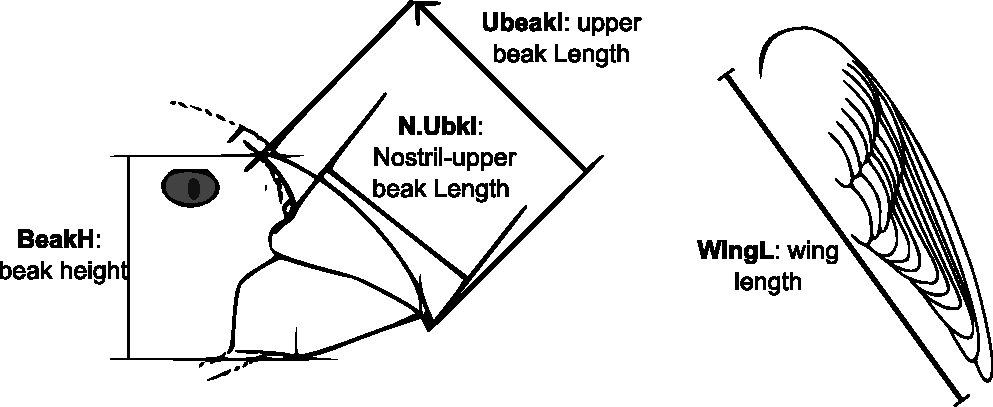
\includegraphics[width=\textwidth]{figs/darwinfinch.pdf}
\end{center}

\newpage


%%%%%%%%%%%%%%%%
\section{Description of traits distributions}
%%%%%%%%%%%%%%%%

\subsection{Plot the kernel density of traits}

Plot the distribution of traits values for populations, species, sites and regional scales. First, let try the distribution for all populations of Darwin finches.

\begin{knitrout}
\definecolor{shadecolor}{rgb}{0.969, 0.969, 0.969}\color{fgcolor}\begin{kframe}
\begin{alltt}
\hlkwd{par}\hlstd{(}\hlkwc{mfrow}\hlstd{=}\hlkwd{c}\hlstd{(}\hlnum{4}\hlstd{,}\hlnum{4}\hlstd{),} \hlkwc{cex}\hlstd{=}\hlnum{0.5}\hlstd{)}
\hlkwd{plotDistri}\hlstd{(traits.finch, sp.finch, ind.plot.finch,}
          \hlkwc{ylim.cex}\hlstd{=}\hlnum{3}\hlstd{,} \hlkwc{plot.ask}\hlstd{=F,} \hlkwc{multipanel}\hlstd{=F,} \hlkwc{leg}\hlstd{=F)}
\end{alltt}
\end{kframe}
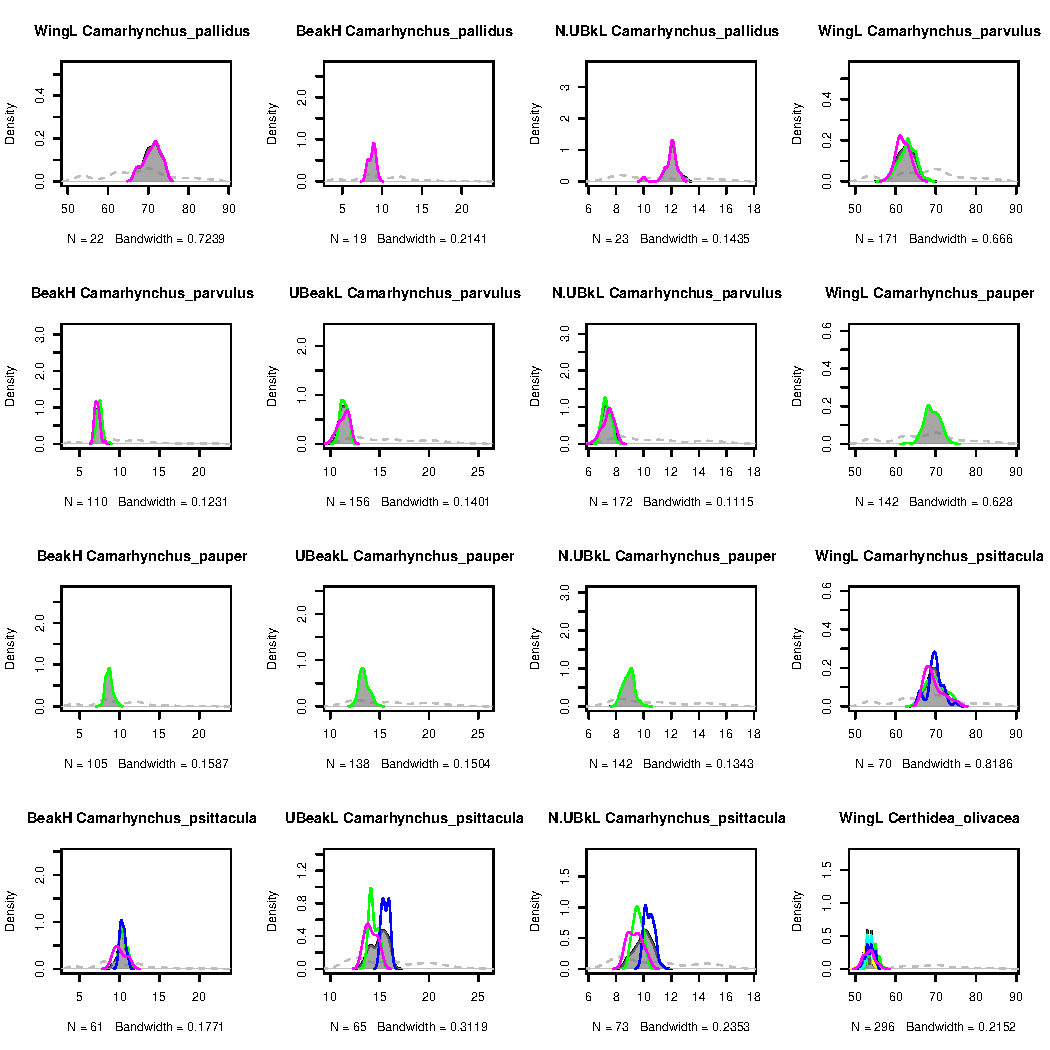
\includegraphics[width=\maxwidth]{figure/unnamed-chunk-101} 

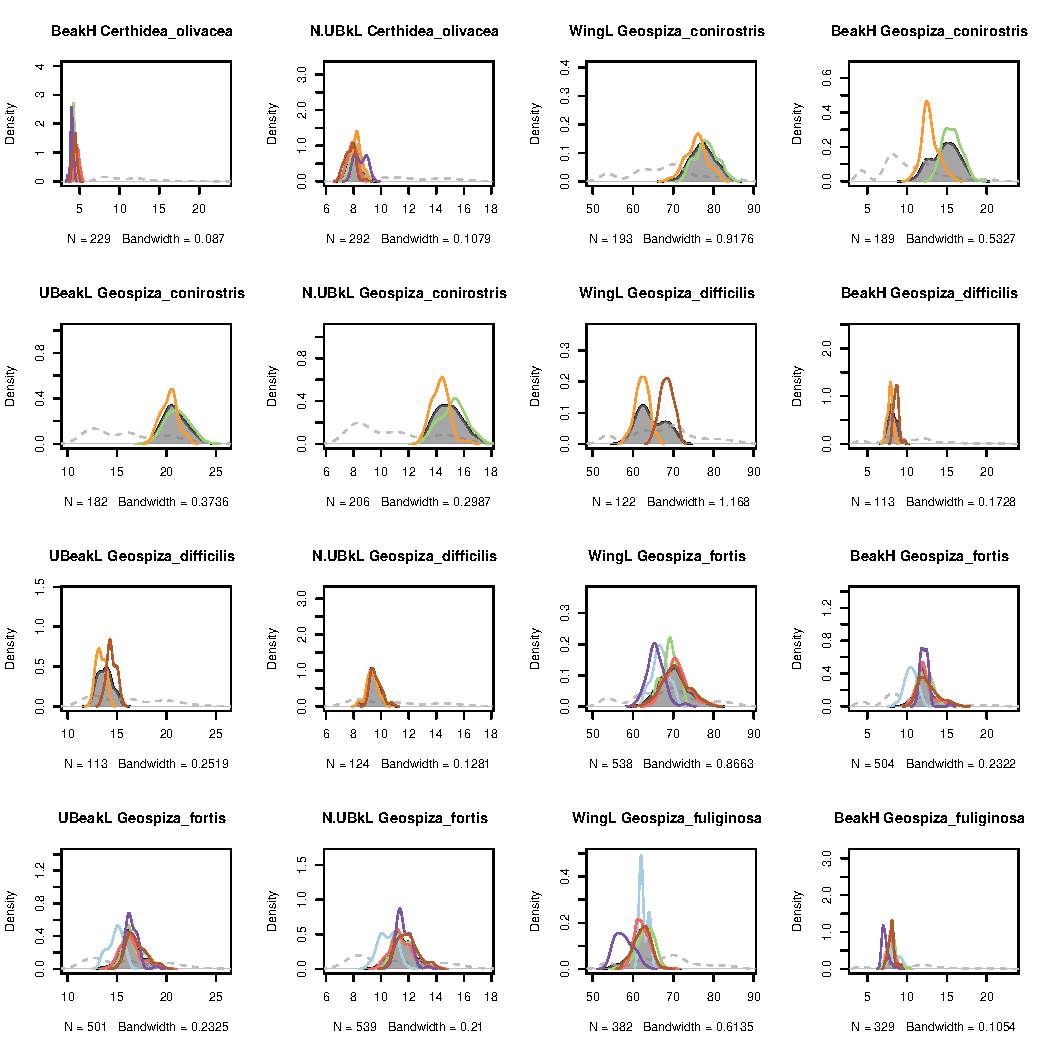
\includegraphics[width=\maxwidth]{figure/unnamed-chunk-102} 

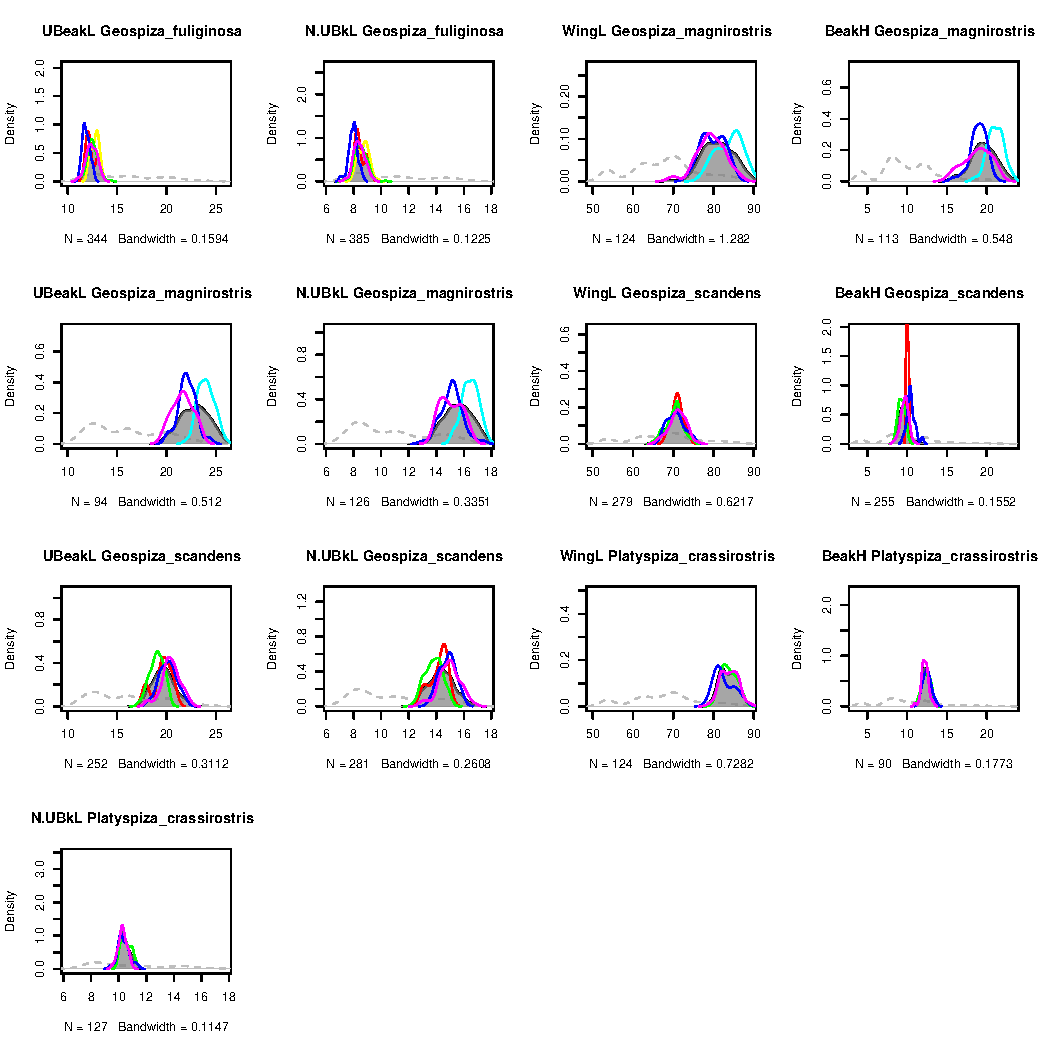
\includegraphics[width=\maxwidth]{figure/unnamed-chunk-103} 

\end{knitrout}

\newpage

Then we can inverse the second and the third arguments to plot the distribution for all finches species. 

\begin{knitrout}
\definecolor{shadecolor}{rgb}{0.969, 0.969, 0.969}\color{fgcolor}\begin{kframe}
\begin{alltt}
\hlkwd{par}\hlstd{(}\hlkwc{mfrow}\hlstd{=}\hlkwd{c}\hlstd{(}\hlnum{4}\hlstd{,}\hlnum{4}\hlstd{),} \hlkwc{cex}\hlstd{=}\hlnum{0.5}\hlstd{)}
\hlkwd{plotDistri}\hlstd{(traits.finch, ind.plot.finch, sp.finch,}
           \hlkwc{ylim.cex}\hlstd{=}\hlnum{8}\hlstd{,} \hlkwc{plot.ask}\hlstd{=F,} \hlkwc{multipanel}\hlstd{=F,} \hlkwc{leg}\hlstd{=F)}
\end{alltt}
\end{kframe}
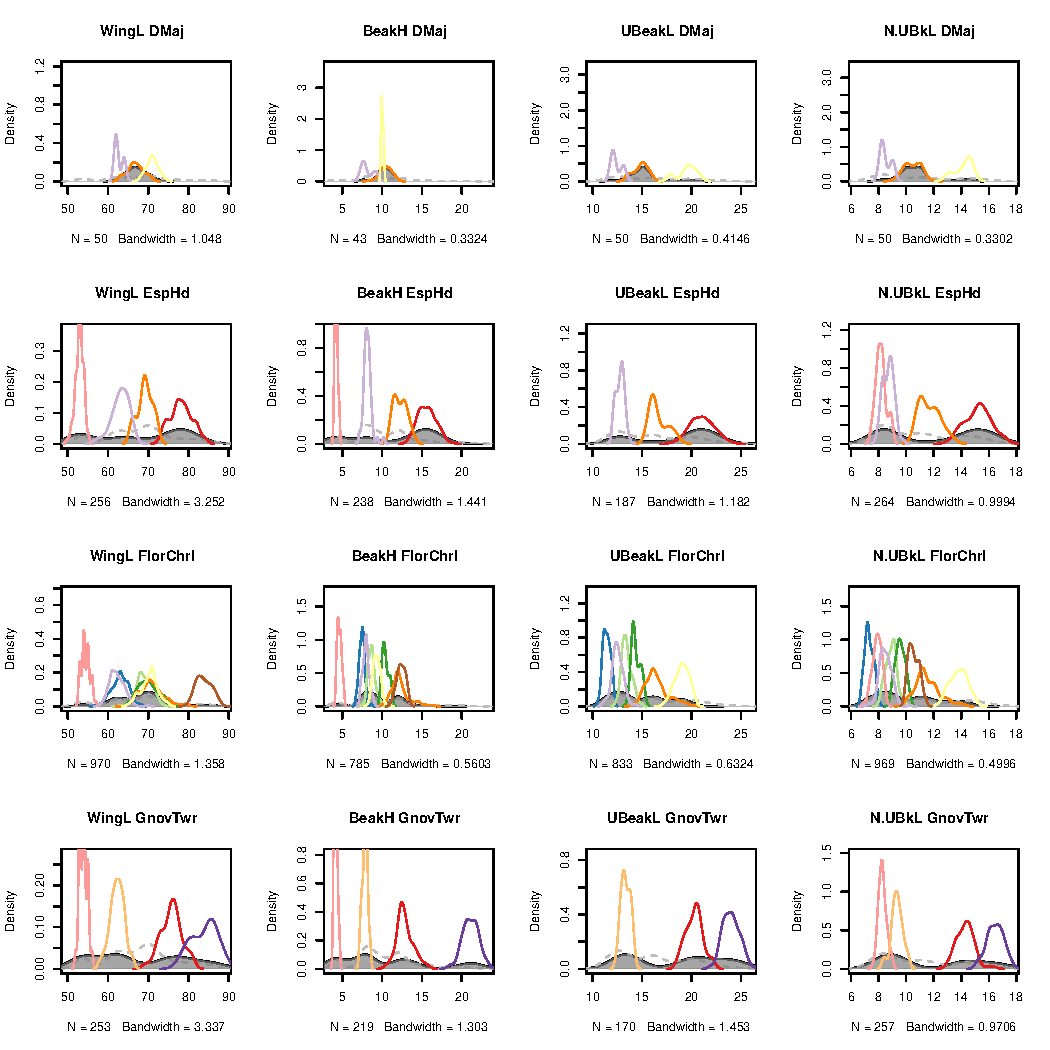
\includegraphics[width=\maxwidth]{figure/unnamed-chunk-111} 

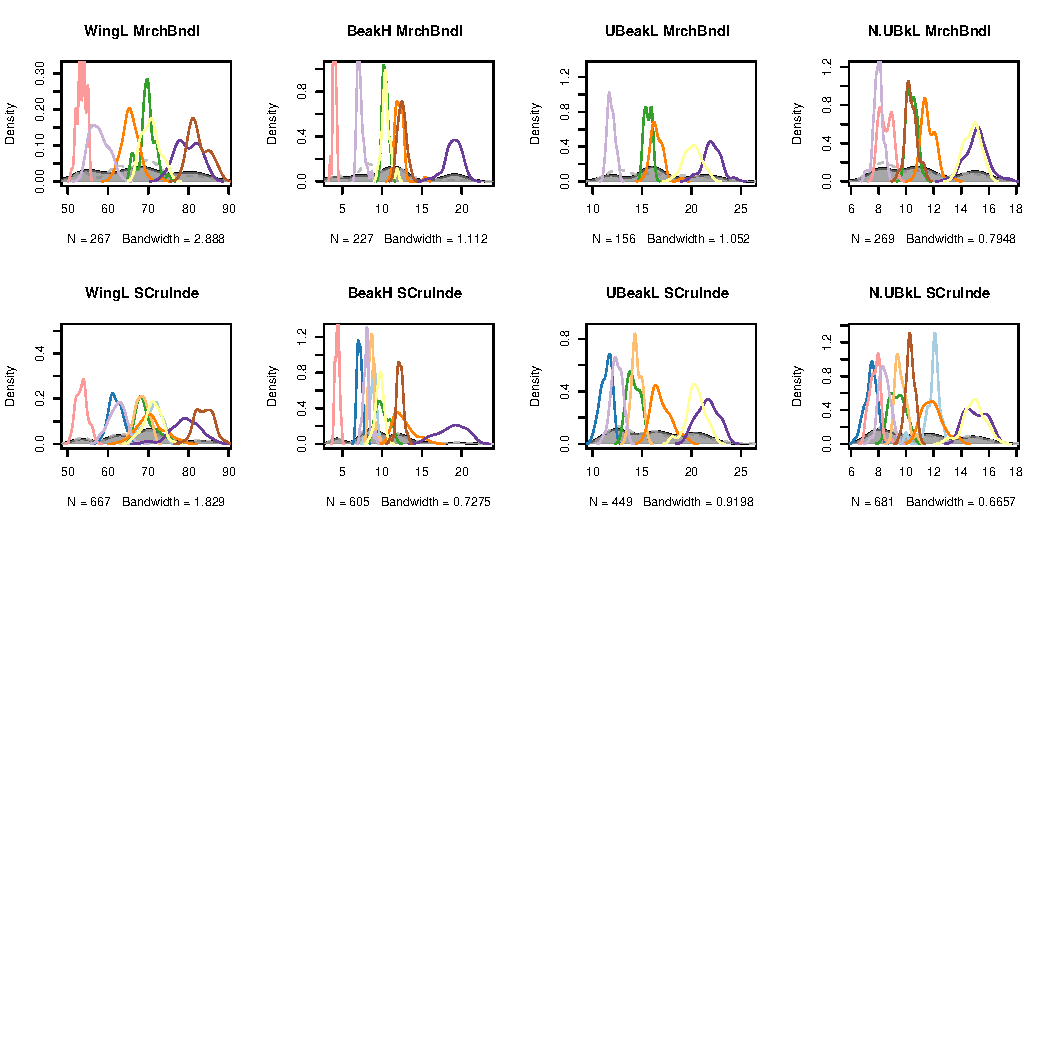
\includegraphics[width=\maxwidth]{figure/unnamed-chunk-112} 

\end{knitrout}

Only one trait to plot using leg=T to plot the legend.

\begin{knitrout}
\definecolor{shadecolor}{rgb}{0.969, 0.969, 0.969}\color{fgcolor}\begin{kframe}
\begin{alltt}
\hlkwd{par}\hlstd{(}\hlkwc{mfrow}\hlstd{=}\hlkwd{c}\hlstd{(}\hlnum{2}\hlstd{,}\hlnum{3}\hlstd{))}
\hlkwd{plotDistri}\hlstd{(}\hlkwd{as.matrix}\hlstd{(traits.finch[,}\hlnum{1}\hlstd{]), ind.plot.finch, sp.finch,}
          \hlkwc{ylim.cex}\hlstd{=}\hlnum{8}\hlstd{,} \hlkwc{plot.ask}\hlstd{=F,} \hlkwc{multipanel}\hlstd{=F,} \hlkwc{leg}\hlstd{=T,} \hlkwc{cex.leg}\hlstd{=}\hlnum{0.5}\hlstd{)}
\end{alltt}
\end{kframe}
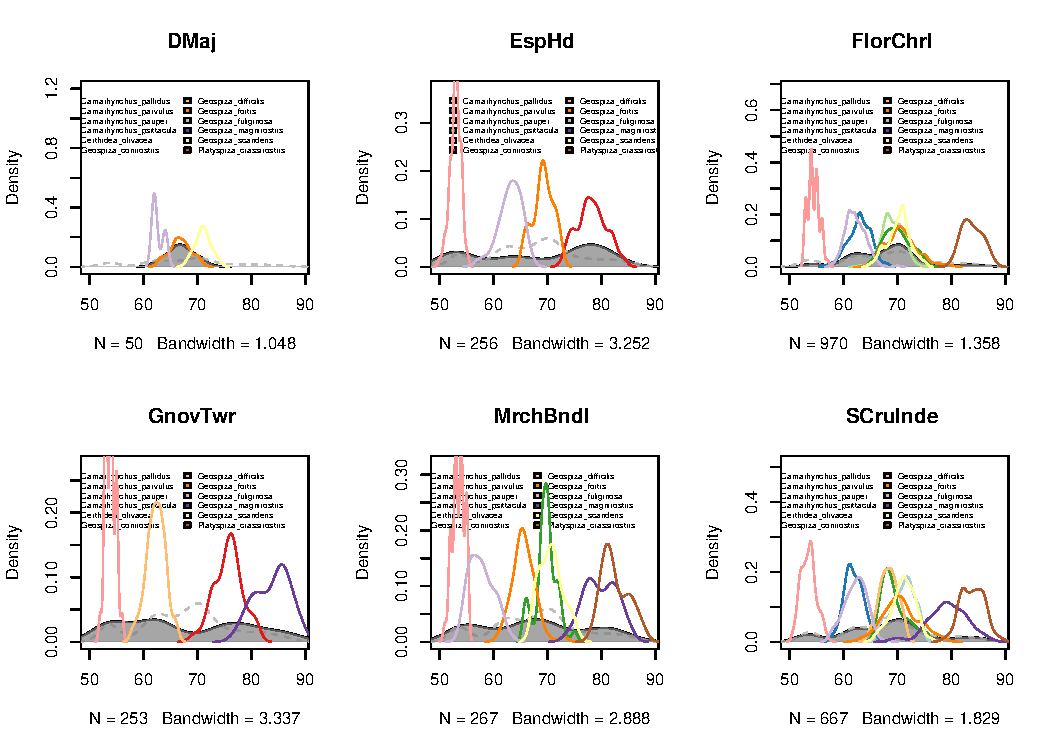
\includegraphics[width=\maxwidth]{figure/unnamed-chunk-12} 

\end{knitrout}

If we want to plot all the sites (regional distribution) or all the species: we can use the folowing code:
\begin{knitrout}
\definecolor{shadecolor}{rgb}{0.969, 0.969, 0.969}\color{fgcolor}\begin{kframe}
\begin{alltt}
\hlkwd{par}\hlstd{(}\hlkwc{mfrow}\hlstd{=}\hlkwd{c}\hlstd{(}\hlnum{4}\hlstd{,}\hlnum{4}\hlstd{),} \hlkwc{cex}\hlstd{=}\hlnum{0.5}\hlstd{)}
\hlkwd{plotDistri}\hlstd{(traits.finch,} \hlkwd{rep}\hlstd{(}\hlstr{"region"}\hlstd{,} \hlkwc{times}\hlstd{=}\hlkwd{dim}\hlstd{(traits.finch)[}\hlnum{1}\hlstd{]),}
          \hlstd{sp.finch,} \hlkwc{ylim.cex}\hlstd{=}\hlnum{6}\hlstd{,} \hlkwc{plot.ask}\hlstd{=F,} \hlkwc{leg}\hlstd{=F)}
\end{alltt}
\end{kframe}
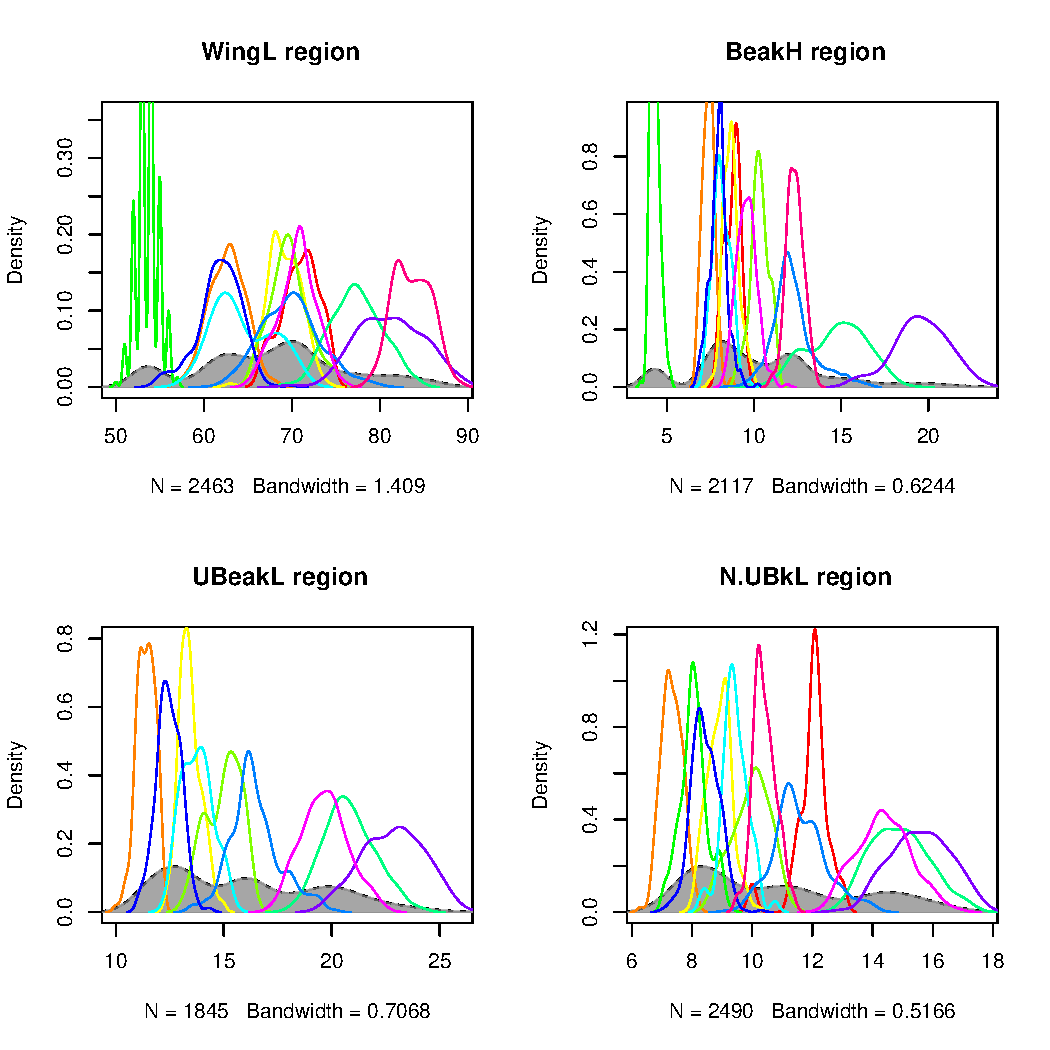
\includegraphics[width=\maxwidth]{figure/unnamed-chunk-13} 

\end{knitrout}

\begin{knitrout}
\definecolor{shadecolor}{rgb}{0.969, 0.969, 0.969}\color{fgcolor}\begin{kframe}
\begin{alltt}
\hlkwd{plotDistri}\hlstd{(traits.finch,} \hlkwd{rep}\hlstd{(}\hlstr{"toutes_sp"}\hlstd{,} \hlkwc{times}\hlstd{=}\hlkwd{dim}\hlstd{(traits.finch)[}\hlnum{1}\hlstd{]),}
          \hlstd{ind.plot.finch,} \hlkwc{ylim.cex}\hlstd{=}\hlnum{3}\hlstd{,} \hlkwc{plot.ask}\hlstd{=F,} \hlkwc{cex.leg}\hlstd{=}\hlnum{0.5}\hlstd{)}
\end{alltt}
\end{kframe}
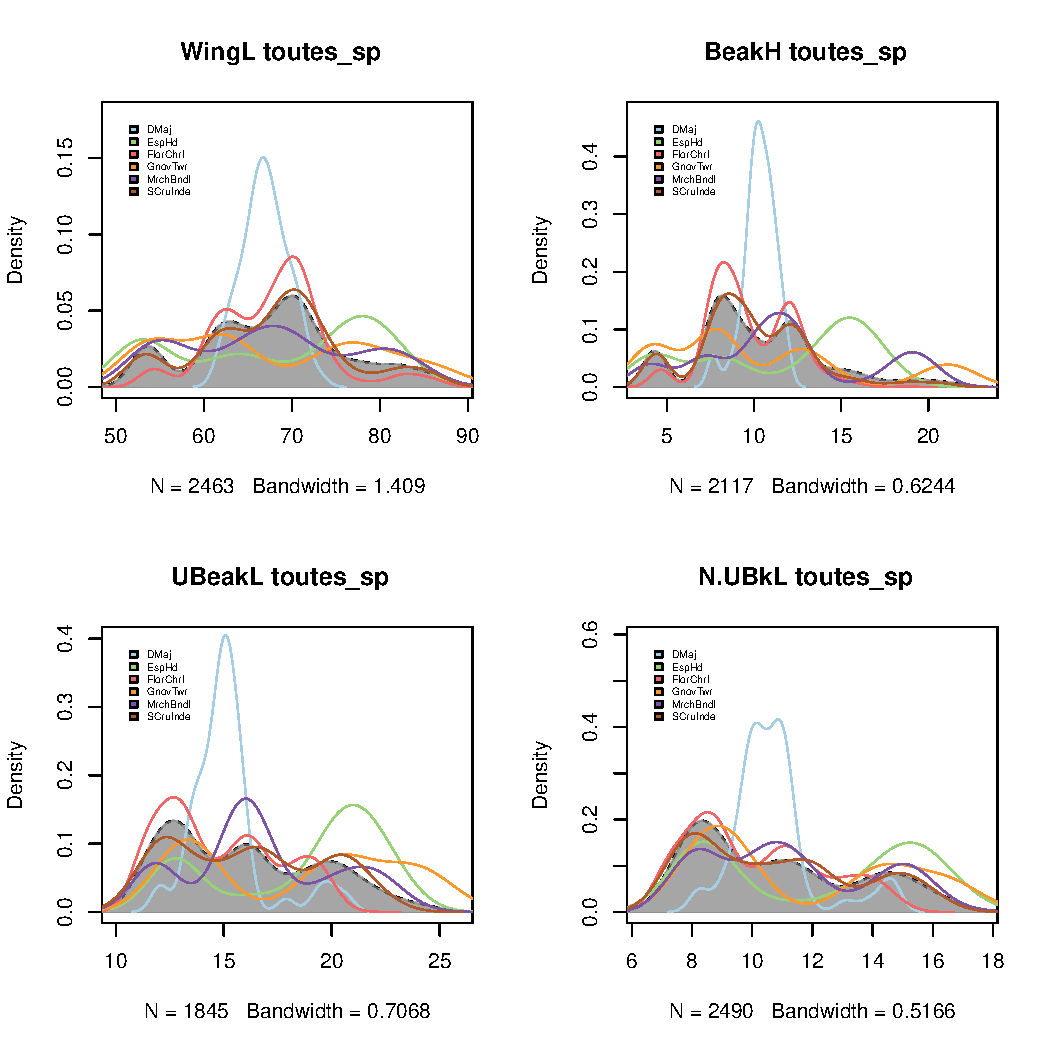
\includegraphics[width=\maxwidth]{figure/unnamed-chunk-14} 

\end{knitrout}

Reset the default parameter
\begin{knitrout}
\definecolor{shadecolor}{rgb}{0.969, 0.969, 0.969}\color{fgcolor}\begin{kframe}
\begin{alltt}
\hlkwd{par}\hlstd{(old.par)}
\end{alltt}
\end{kframe}
\end{knitrout}
\newpage

%%%%%%%%%%%%%%%%
\section{Decomposition of variances}
%%%%%%%%%%%%%%%%

\subsection{Decomposition of within/among species variances using rao diversity}

The Rao function computes α, γ and β -components for taxonomic, functional and/or phylogenetic diversity with:

\begin{center}
$\gamma = mean \alpha + \beta$
\end{center}

Where: \gamma is the diversity of the regional pool, \alpha is the diversity of the local community and \beta is the turn over between local communities; diversity is estimated using the Rao quadratic entropy indices.
\\

\textbf{Reference}: de Bello, F., Lavorel, S., Albert, C.H., Thuiller, W., Grigulis, K., Dolezal, J., Janecek, S. and Leps, J. (2011) Quantifying the relevance of intraspecific trait variability for functional diversity. Methods in Ecology and Evolution, 2, 163-174.


\subsubsection{Multitraits analysis}
First, rao diversity can be calculated on the functionnal space (i.e. considering all traits together).

\begin{knitrout}
\definecolor{shadecolor}{rgb}{0.969, 0.969, 0.969}\color{fgcolor}\begin{kframe}
\begin{alltt}
\hlcom{#create individuals community matrix}
\hlstd{comm}\hlkwb{<-}\hlkwd{t}\hlstd{(}\hlkwd{table}\hlstd{(ind.plot.finch,}\hlnum{1}\hlopt{:}\hlkwd{length}\hlstd{(ind.plot.finch)))}
\hlcom{#create species community matrix}
\hlstd{comm.sp}\hlkwb{<-}\hlkwd{table}\hlstd{(sp.finch, ind.plot.finch)}
\hlkwd{class}\hlstd{(comm.sp)}\hlkwb{<-}\hlstr{"matrix"}

\hlstd{traits.finch.sp}\hlkwb{<-}\hlkwd{apply}\hlstd{(} \hlkwd{apply}\hlstd{(traits.finch,} \hlnum{2}\hlstd{, scale ),} \hlnum{2}\hlstd{,}
                        \hlkwa{function}\hlstd{(}\hlkwc{x}\hlstd{)} \hlkwd{tapply}\hlstd{(x, sp.finch, mean,} \hlkwc{na.rm}\hlstd{=T))}

\hlstd{mat.dist}\hlkwb{<-}\hlkwd{as.matrix}\hlstd{(}\hlkwd{dist}\hlstd{(traits.finch.sp))}\hlopt{^}\hlnum{2}

\hlstd{res.rao}\hlkwb{<-}\hlkwd{RaoRel}\hlstd{(}\hlkwc{sample}\hlstd{=}\hlkwd{as.matrix}\hlstd{(comm.sp),}
                \hlkwc{dfunc}\hlstd{=mat.dist,} \hlkwc{dphyl}\hlstd{=}\hlkwa{NULL}\hlstd{,}
                \hlkwc{weight}\hlstd{=F,} \hlkwc{Jost}\hlstd{=F,} \hlkwc{structure}\hlstd{=}\hlkwa{NULL}\hlstd{)}

\hlstd{witRao}\hlkwb{<-}\hlstd{res.rao}\hlopt{$}\hlstd{FD}\hlopt{$}\hlstd{Mean_Alpha}  \hlcom{#overall within species variance}
\hlstd{betRao}\hlkwb{<-}\hlstd{res.rao}\hlopt{$}\hlstd{FD}\hlopt{$}\hlstd{Beta_add}    \hlcom{#between species variance}
\hlstd{totRao}\hlkwb{<-}\hlstd{res.rao}\hlopt{$}\hlstd{FD}\hlopt{$}\hlstd{Gamma}       \hlcom{#the total variance}

\hlstd{witRao}\hlopt{+}\hlstd{betRao}
\end{alltt}
\begin{verbatim}
## [1] 8.37
\end{verbatim}
\begin{alltt}
\hlstd{totRao}
\end{alltt}
\begin{verbatim}
## [1] 8.37
\end{verbatim}
\end{kframe}
\end{knitrout}

Now let's take the abundance to calculate Rao diversity.

\begin{knitrout}
\definecolor{shadecolor}{rgb}{0.969, 0.969, 0.969}\color{fgcolor}\begin{kframe}
\begin{alltt}
\hlstd{res.rao.w}\hlkwb{<-}\hlkwd{RaoRel}\hlstd{(}\hlkwc{sample}\hlstd{=}\hlkwd{as.matrix}\hlstd{(comm.sp),}
                  \hlkwc{dfunc}\hlstd{=mat.dist,} \hlkwc{dphyl}\hlstd{=}\hlkwa{NULL}\hlstd{,}
                  \hlkwc{weight}\hlstd{=T,} \hlkwc{Jost}\hlstd{=F,} \hlkwc{structure}\hlstd{=}\hlkwa{NULL}\hlstd{)}

\hlstd{witRao.w}\hlkwb{<-}\hlstd{res.rao.w}\hlopt{$}\hlstd{FD}\hlopt{$}\hlstd{Mean_Alpha}  \hlcom{#overall within species variance}
\hlstd{betRao.w}\hlkwb{<-}\hlstd{res.rao.w}\hlopt{$}\hlstd{FD}\hlopt{$}\hlstd{Beta_add}    \hlcom{#between species variance}
\hlstd{totRao.w}\hlkwb{<-}\hlstd{res.rao.w}\hlopt{$}\hlstd{FD}\hlopt{$}\hlstd{Gamma}       \hlcom{#the total variance}

\hlstd{witRao.w}
\end{alltt}
\begin{verbatim}
## [1] 7.551
\end{verbatim}
\begin{alltt}
\hlstd{betRao.w}
\end{alltt}
\begin{verbatim}
## [1] 0.3458
\end{verbatim}
\end{kframe}
\end{knitrout}

Plot the results

\begin{knitrout}
\definecolor{shadecolor}{rgb}{0.969, 0.969, 0.969}\color{fgcolor}\begin{kframe}
\begin{alltt}
\hlkwd{barplot}\hlstd{(}\hlkwd{cbind}\hlstd{(}\hlkwd{c}\hlstd{(witRao.w, betRao.w),} \hlkwd{c}\hlstd{(witRao, betRao)),}
        \hlkwc{names.arg} \hlstd{=}\hlkwd{c}\hlstd{(}\hlstr{"abundance"} \hlstd{,}\hlstr{"presence"}\hlstd{),}
        \hlkwc{legend.text}\hlstd{=}\hlkwd{c}\hlstd{(}\hlstr{"within species"}\hlstd{,} \hlstr{"between species"}\hlstd{),}
        \hlkwc{ylab}\hlstd{=}\hlstr{"Rao"}\hlstd{,} \hlkwc{ylim}\hlstd{=}\hlkwd{c}\hlstd{(}\hlnum{0}\hlstd{,}\hlnum{10}\hlstd{))}
\end{alltt}
\end{kframe}

{\centering 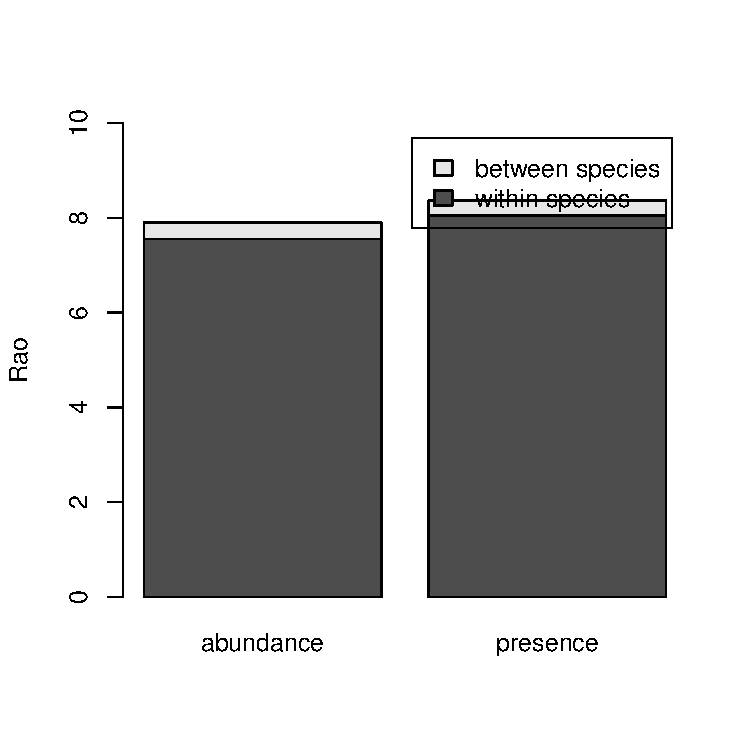
\includegraphics[width=\maxwidth]{figure/unnamed-chunk-18} 

}



\end{knitrout}


\subsubsection{Unitraits analysis}
We can also do this analysis for each trait separately. We need to replace (or exclude) NA values. For this example, we use the package mice to complete the data.

\begin{knitrout}
\definecolor{shadecolor}{rgb}{0.969, 0.969, 0.969}\color{fgcolor}\begin{kframe}
\begin{alltt}
\hlstd{comm}\hlkwb{<-}\hlkwd{t}\hlstd{(}\hlkwd{table}\hlstd{(ind.plot.finch,}\hlnum{1}\hlopt{:}\hlkwd{length}\hlstd{(ind.plot.finch)))}

\hlkwd{require}\hlstd{(mice)}
\hlstd{traits}\hlkwb{=}\hlstd{traits.finch}
\hlstd{mice}\hlkwb{<-}\hlkwd{mice}\hlstd{(traits.finch)}
\hlstd{traits.finch.mice}\hlkwb{<-}\hlkwd{complete}\hlstd{(mice)}
\end{alltt}
\end{kframe}
\end{knitrout}


\begin{knitrout}
\definecolor{shadecolor}{rgb}{0.969, 0.969, 0.969}\color{fgcolor}\begin{kframe}
\begin{alltt}
\hlcom{#Calculate the mean traits value by population using the mice dataset}
\hlstd{traits.finch.mice.sp}\hlkwb{<-}\hlkwd{apply}\hlstd{(}\hlkwd{apply}\hlstd{(traits.finch.mice,} \hlnum{2}\hlstd{, scale ),} \hlnum{2}\hlstd{,}
                            \hlkwa{function}\hlstd{(}\hlkwc{x}\hlstd{)} \hlkwd{tapply}\hlstd{(x, sp.finch, mean,} \hlkwc{na.rm}\hlstd{=T))}

\hlstd{trait.rao.w}\hlkwb{<-}\hlkwd{list}\hlstd{()}
\hlstd{witRao.w.bytrait}\hlkwb{<-}\hlkwd{c}\hlstd{()}
\hlstd{betRao.w.bytrait}\hlkwb{<-}\hlkwd{c}\hlstd{()}
\hlkwa{for}\hlstd{(t} \hlkwa{in} \hlnum{1} \hlopt{:} \hlnum{4}\hlstd{)\{}
  \hlstd{trait.rao.w[[t]]}\hlkwb{<-}\hlkwd{RaoRel}\hlstd{(}\hlkwc{sample}\hlstd{=}\hlkwd{as.matrix}\hlstd{(comm.sp),}
                           \hlkwc{dfunc}\hlstd{=}\hlkwd{dist}\hlstd{(traits.finch.mice.sp[,t]),}
                           \hlkwc{dphyl}\hlstd{=}\hlkwa{NULL}\hlstd{,} \hlkwc{weight}\hlstd{=T,} \hlkwc{Jost}\hlstd{=F,} \hlkwc{structure}\hlstd{=}\hlkwa{NULL}\hlstd{)}
  \hlstd{witRao.w.bytrait}\hlkwb{<-}\hlkwd{c}\hlstd{(witRao.w.bytrait, trait.rao.w[[t]]}\hlopt{$}\hlstd{FD}\hlopt{$}\hlstd{Mean_Alpha)}
  \hlstd{betRao.w.bytrait}\hlkwb{<-}\hlkwd{c}\hlstd{(betRao.w.bytrait, trait.rao.w[[t]]}\hlopt{$}\hlstd{FD}\hlopt{$}\hlstd{Beta_add)}
\hlstd{\}}
\end{alltt}
\end{kframe}
\end{knitrout}

Plot the results by traits.

\begin{knitrout}
\definecolor{shadecolor}{rgb}{0.969, 0.969, 0.969}\color{fgcolor}\begin{kframe}
\begin{alltt}
\hlkwd{barplot}\hlstd{(}\hlkwd{t}\hlstd{(}\hlkwd{cbind}\hlstd{( witRao.w.bytrait, betRao.w.bytrait)),}
        \hlkwc{names.arg} \hlstd{=} \hlkwd{colnames}\hlstd{(traits.finch),}
        \hlkwc{legend.text}\hlstd{=}\hlkwd{c}\hlstd{(}\hlstr{"within species"}\hlstd{,} \hlstr{"between species"}\hlstd{),}
        \hlkwc{ylab}\hlstd{=}\hlstr{"Rao"}\hlstd{,} \hlkwc{ylim}\hlstd{=}\hlkwd{c}\hlstd{(}\hlnum{0}\hlstd{,}\hlnum{1.5}\hlstd{))}
\end{alltt}
\end{kframe}
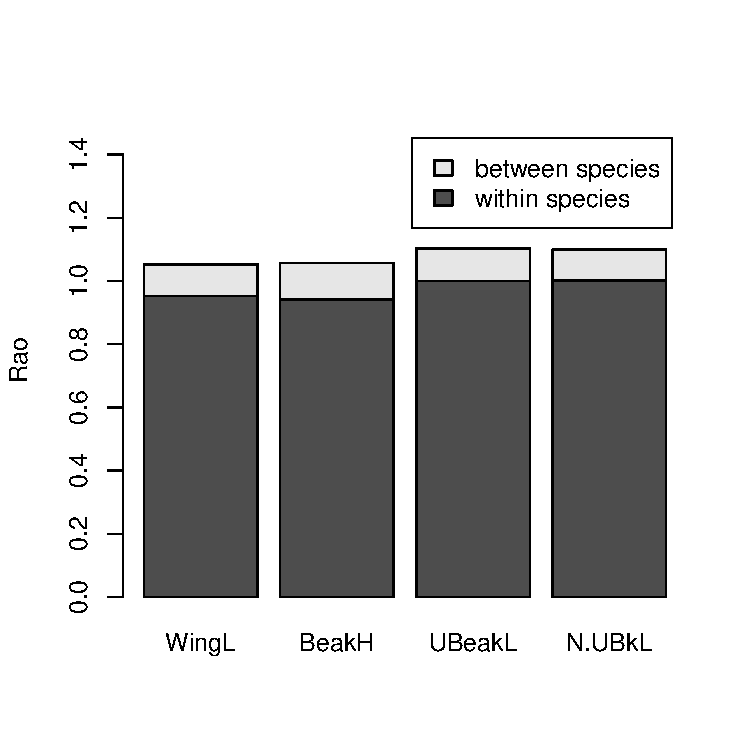
\includegraphics[width=\maxwidth]{figure/unnamed-chunk-21} 

\end{knitrout}


\subsection{Decomposition of community trait response to environment into intraspecific trait variability, variability due to species turnover and their covariation.}

\textbf{Reference}: Leps, J., de Bello, F., Smilauer, P. and Dolezal, J. (2011) Community trait response to environment: disentangling species turnover vs intraspecific trait variability effects. Ecography, 34, 856-863.

\begin{knitrout}
\definecolor{shadecolor}{rgb}{0.969, 0.969, 0.969}\color{fgcolor}\begin{kframe}
\begin{alltt}
\hlstd{res.decomp}\hlkwb{<-}\hlkwd{decompCTRE}\hlstd{(}\hlkwc{traits}\hlstd{=traits.finch,} \hlkwc{sp}\hlstd{=sp.finch,}
                           \hlkwc{ind.plot}\hlstd{=ind.plot.finch,} \hlkwc{print}\hlstd{=}\hlnum{FALSE}\hlstd{)}

\hlkwd{barplot}\hlstd{(res.decomp)}
\end{alltt}
\end{kframe}

{\centering 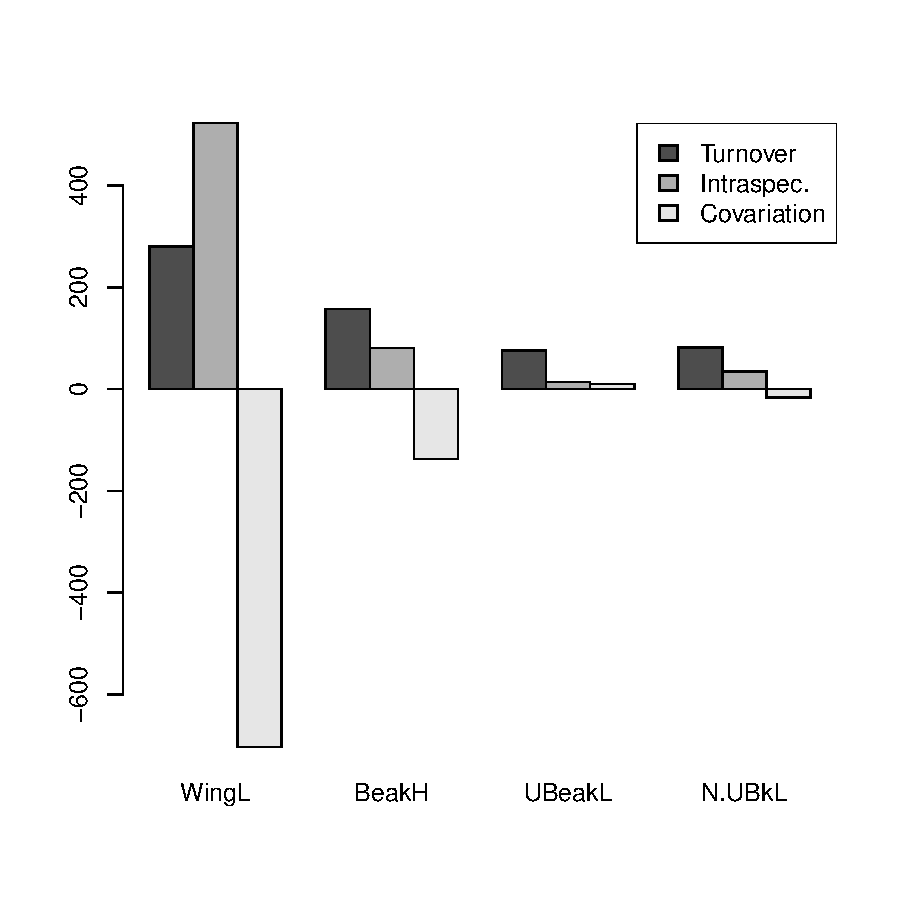
\includegraphics[width=\maxwidth]{figure/unnamed-chunk-221} 

}


\begin{kframe}\begin{alltt}
\hlkwd{par}\hlstd{(}\hlkwc{mfrow}\hlstd{=}\hlkwd{c}\hlstd{(}\hlnum{2}\hlstd{,}\hlnum{2}\hlstd{))}
\hlkwd{barplot}\hlstd{(res.decomp,} \hlkwc{resume}\hlstd{=F)}
\end{alltt}
\end{kframe}

{\centering 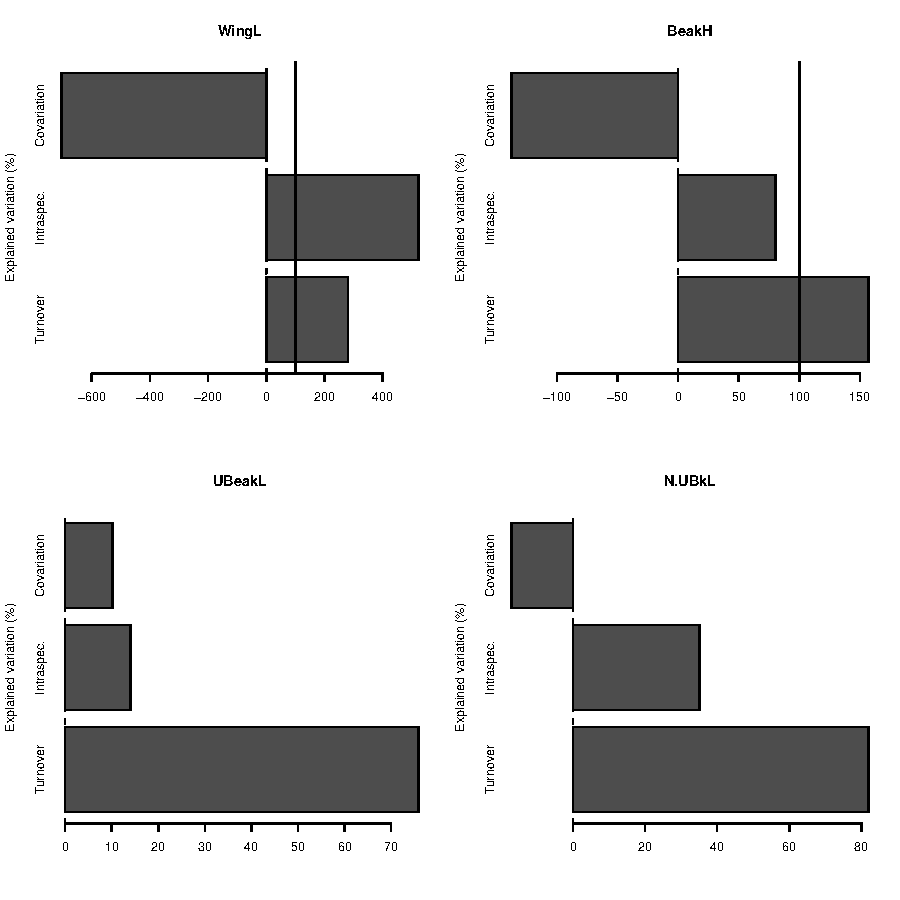
\includegraphics[width=\maxwidth]{figure/unnamed-chunk-222} 

}


\begin{kframe}\begin{alltt}
\hlkwd{par}\hlstd{(}\hlkwc{mfrow}\hlstd{=}\hlkwd{c}\hlstd{(}\hlnum{1}\hlstd{,}\hlnum{1}\hlstd{))}
\end{alltt}
\end{kframe}
\end{knitrout}

\newpage

\subsection{Decomposition of traits variances using nested factors}

Variance partitioning across nested scales using the decomposition of variance on restricted maximum likelihood (REML) method (lme function).
\\

\textbf{Reference}: Messier, J., McGill, B. and Lechowicz, M. (2010) How do traits vary across ecological scales? A case for trait-based ecology. Ecology Letters, 13, 838-848.

\begin{knitrout}
\definecolor{shadecolor}{rgb}{0.969, 0.969, 0.969}\color{fgcolor}\begin{kframe}
\begin{alltt}
\hlstd{vec}\hlkwb{<-} \hlkwd{seq}\hlstd{(}\hlnum{1}\hlstd{,}\hlkwd{length}\hlstd{(sp.finch)}\hlopt{*}\hlnum{2}\hlstd{,} \hlkwc{by}\hlstd{=}\hlnum{2}\hlstd{)}
\hlstd{genus}\hlkwb{<-}\hlkwd{as.vector}\hlstd{(}\hlkwd{unlist}\hlstd{(}\hlkwd{strsplit}\hlstd{(}\hlkwd{as.vector}\hlstd{(sp.finch),}\hlstr{"_"}\hlstd{))[vec])}
\hlstd{fact}\hlkwb{<-}\hlkwd{cbind}\hlstd{(}\hlkwc{genus}\hlstd{=}\hlkwd{as.factor}\hlstd{(genus),}
            \hlkwc{species}\hlstd{=}\hlkwd{as.factor}\hlstd{(}\hlkwd{as.vector}\hlstd{(sp.finch)),}
            \hlkwc{sites}\hlstd{=}\hlkwd{as.factor}\hlstd{(}\hlkwd{as.vector}\hlstd{(ind.plot.finch)))}

\hlstd{res.partvar.finch}\hlkwb{<-}\hlkwd{partvar}\hlstd{(}\hlkwc{traits}\hlstd{=traits.finch,} \hlkwc{factors}\hlstd{=fact)}

\hlstd{res.partvar.finch}
\end{alltt}
\end{kframe}
\end{knitrout}


\begin{knitrout}
\definecolor{shadecolor}{rgb}{0.969, 0.969, 0.969}\color{fgcolor}\begin{kframe}
\begin{alltt}
\hlkwd{par}\hlstd{(}\hlkwc{mfrow}\hlstd{=}\hlkwd{c}\hlstd{(}\hlnum{2}\hlstd{,}\hlnum{2}\hlstd{),} \hlkwc{mai}\hlstd{=}\hlkwd{c}\hlstd{(}\hlnum{0.2}\hlstd{,}\hlnum{0.2}\hlstd{,}\hlnum{0.2}\hlstd{,}\hlnum{0.2}\hlstd{))}
\hlstd{colors}\hlkwb{<-}\hlkwd{c}\hlstd{(}\hlkwd{rgb}\hlstd{(}\hlnum{102}\hlstd{,}\hlnum{167}\hlstd{,}\hlnum{0}\hlstd{,}  \hlkwc{maxColorValue} \hlstd{=} \hlnum{255}\hlstd{),}
          \hlkwd{rgb}\hlstd{(}\hlnum{185}\hlstd{,}\hlnum{210}\hlstd{,}\hlnum{0}\hlstd{,}  \hlkwc{maxColorValue} \hlstd{=} \hlnum{255}\hlstd{),}
          \hlkwd{rgb}\hlstd{(}\hlnum{98}\hlstd{,}\hlnum{174}\hlstd{,}\hlnum{255}\hlstd{,}  \hlkwc{maxColorValue} \hlstd{=} \hlnum{255}\hlstd{),}
          \hlkwd{rgb}\hlstd{(}\hlnum{158}\hlstd{,}\hlnum{30}\hlstd{,}\hlnum{240}\hlstd{,}  \hlkwc{maxColorValue} \hlstd{=} \hlnum{255}\hlstd{))}

\hlkwd{piePartvar}\hlstd{(res.partvar.finch,} \hlkwc{col}\hlstd{=colors)}
\end{alltt}
\end{kframe}

{\centering 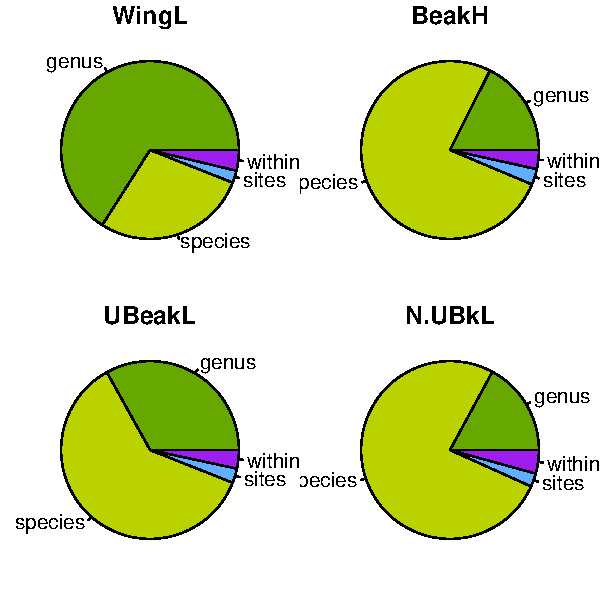
\includegraphics[width=\maxwidth]{figure/unnamed-chunk-241} 

}


\begin{kframe}\begin{alltt}
\hlkwd{par}\hlstd{(old.par)}
\hlkwd{barPartvar}\hlstd{(res.partvar.finch,} \hlkwc{col}\hlstd{=colors,}
            \hlkwc{leg}\hlstd{=}\hlnum{TRUE}\hlstd{)}
\end{alltt}
\end{kframe}

{\centering 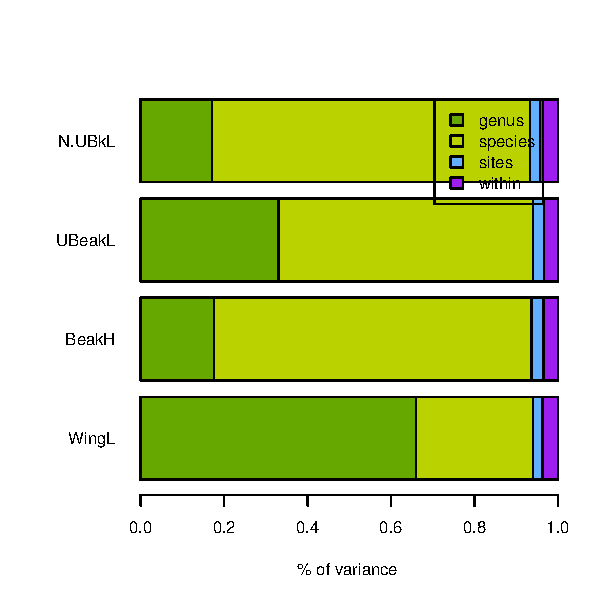
\includegraphics[width=\maxwidth]{figure/unnamed-chunk-242} 

}



\end{knitrout}



\newpage

\subsection{Plot the relation between populational trait means and sites traits means.}

For an example of utilisation see: Cornwell, W.K. and Ackerly, D.D., 2009. Community assembly and shifts in plant trait distributions across an environmental gradient in coastal California. Ecological Monographs 79, 109-126.

\begin{knitrout}
\definecolor{shadecolor}{rgb}{0.969, 0.969, 0.969}\color{fgcolor}\begin{kframe}
\begin{alltt}
\hlkwd{plotSpPop}\hlstd{(traits.finch, ind.plot.finch, sp.finch,} \hlkwc{silent}\hlstd{=}\hlnum{TRUE}\hlstd{)}
\end{alltt}
\end{kframe}
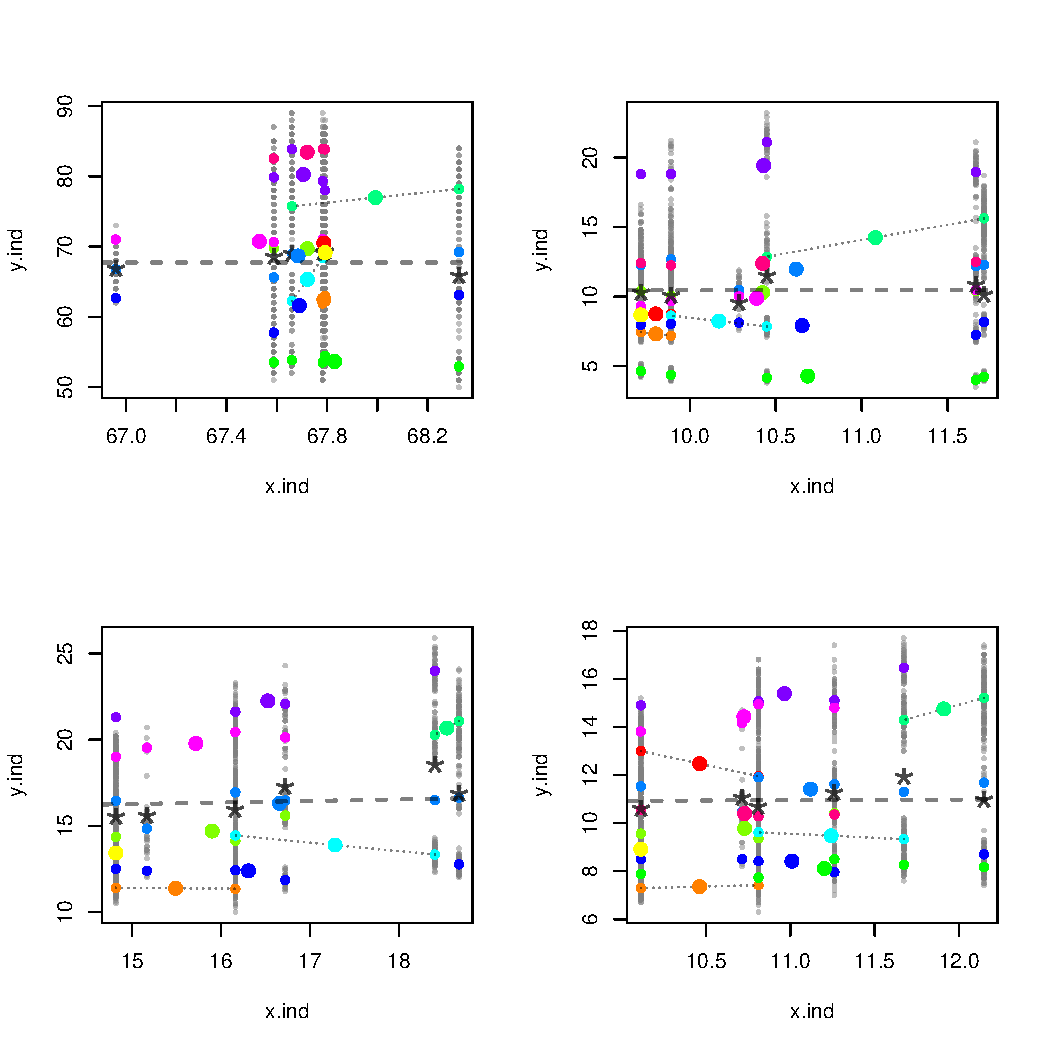
\includegraphics[width=\maxwidth]{figure/unnamed-chunk-25} 

\end{knitrout}

If we change the value of the threshold (alpha=10\% instead of 5\% and the minimum individual to represent singificativity fixed to 3 instead of 10 by default) we can see some significant relationships.

\newpage

\begin{knitrout}
\definecolor{shadecolor}{rgb}{0.969, 0.969, 0.969}\color{fgcolor}\begin{kframe}
\begin{alltt}
\hlkwd{plotSpPop}\hlstd{(traits.finch, ind.plot.finch, sp.finch,}
           \hlkwc{p.val}\hlstd{=}\hlnum{0.1}\hlstd{,}  \hlkwc{min.ind.signif}\hlstd{=}\hlnum{3}\hlstd{,} \hlkwc{silent}\hlstd{=}\hlnum{TRUE}\hlstd{)}
\end{alltt}
\end{kframe}
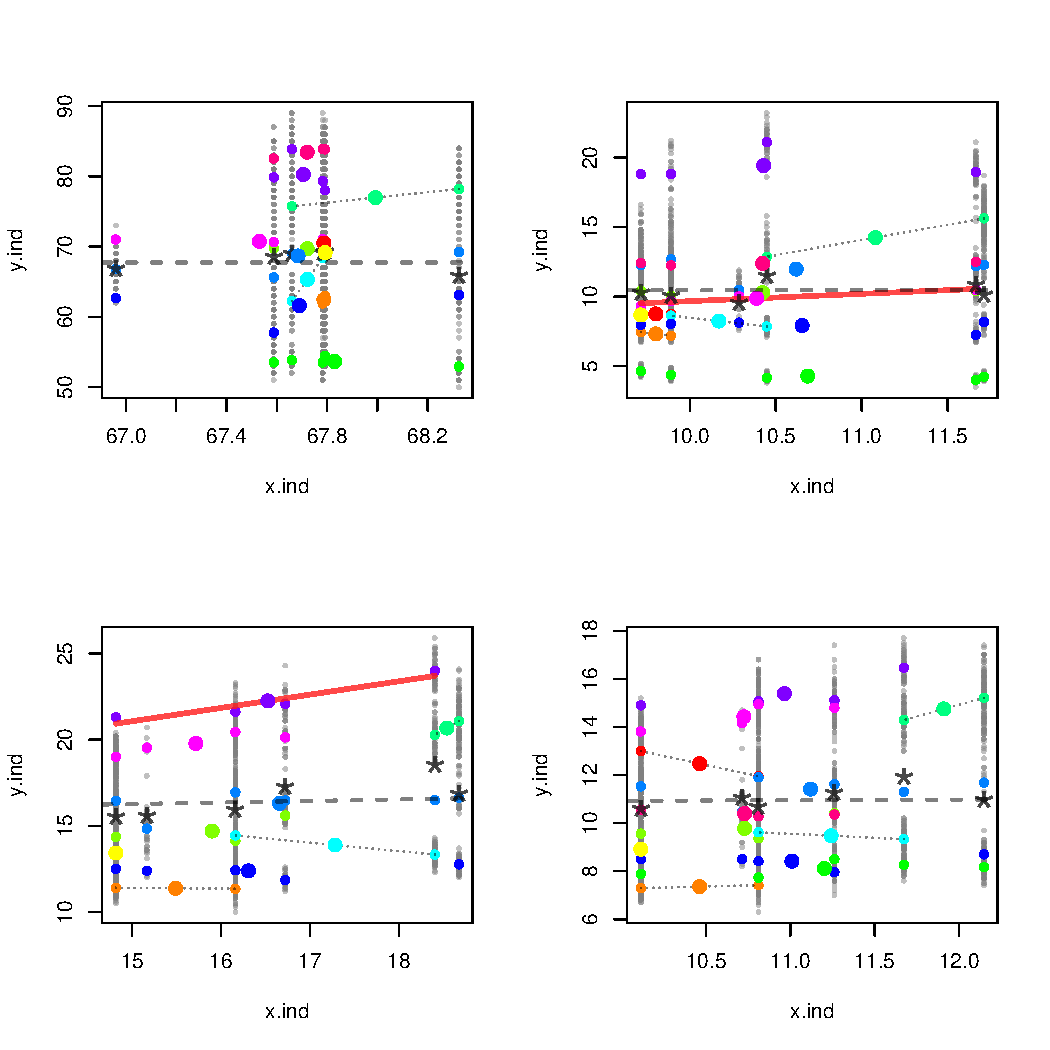
\includegraphics[width=\maxwidth]{figure/unnamed-chunk-26} 

\end{knitrout}

\newpage

For a more simple figure, add the option resume=TRUE. Again if we change the value of the threshold (alpha=10\% instead of 5\% and the minimum individual to represent singificativity fixed to 3 instead of 10 by default) we can see some significant relationships.

\begin{knitrout}
\definecolor{shadecolor}{rgb}{0.969, 0.969, 0.969}\color{fgcolor}\begin{kframe}
\begin{alltt}
\hlkwd{plotSpPop}\hlstd{(traits.finch, ind.plot.finch, sp.finch,}
           \hlkwc{silent}\hlstd{=}\hlnum{TRUE}\hlstd{,} \hlkwc{resume}\hlstd{=}\hlnum{TRUE}\hlstd{,} \hlkwc{col.pop}\hlstd{=}\hlstr{"grey"}\hlstd{)}
\end{alltt}
\end{kframe}
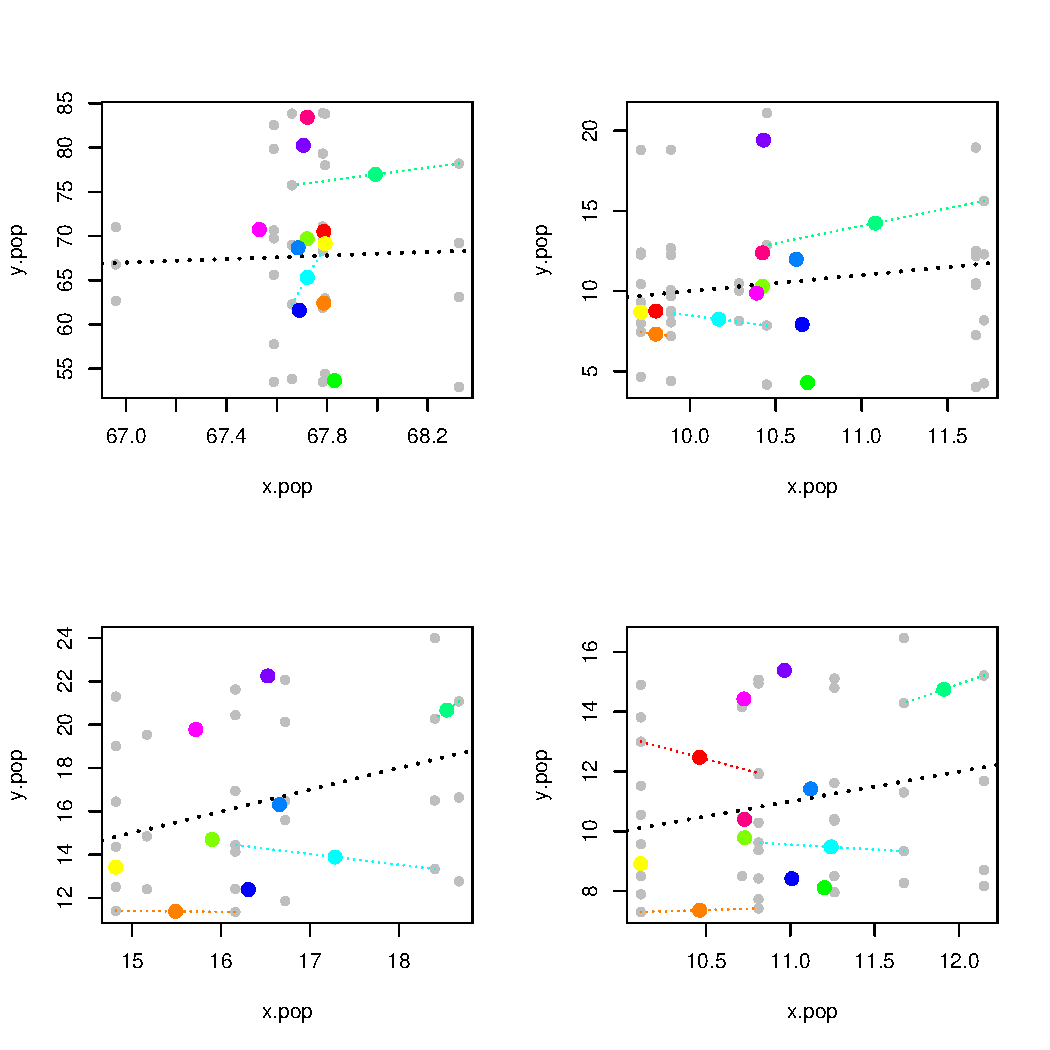
\includegraphics[width=\maxwidth]{figure/unnamed-chunk-271} 
\begin{kframe}\begin{alltt}
\hlkwd{plotSpPop}\hlstd{(traits.finch, ind.plot.finch, sp.finch,}
           \hlkwc{silent}\hlstd{=}\hlnum{TRUE}\hlstd{,} \hlkwc{resume}\hlstd{=}\hlnum{TRUE}\hlstd{,} \hlkwc{col.pop}\hlstd{=}\hlstr{"grey"}\hlstd{,} \hlkwc{col.sp}\hlstd{=}\hlstr{"black"}\hlstd{)}
\end{alltt}
\end{kframe}
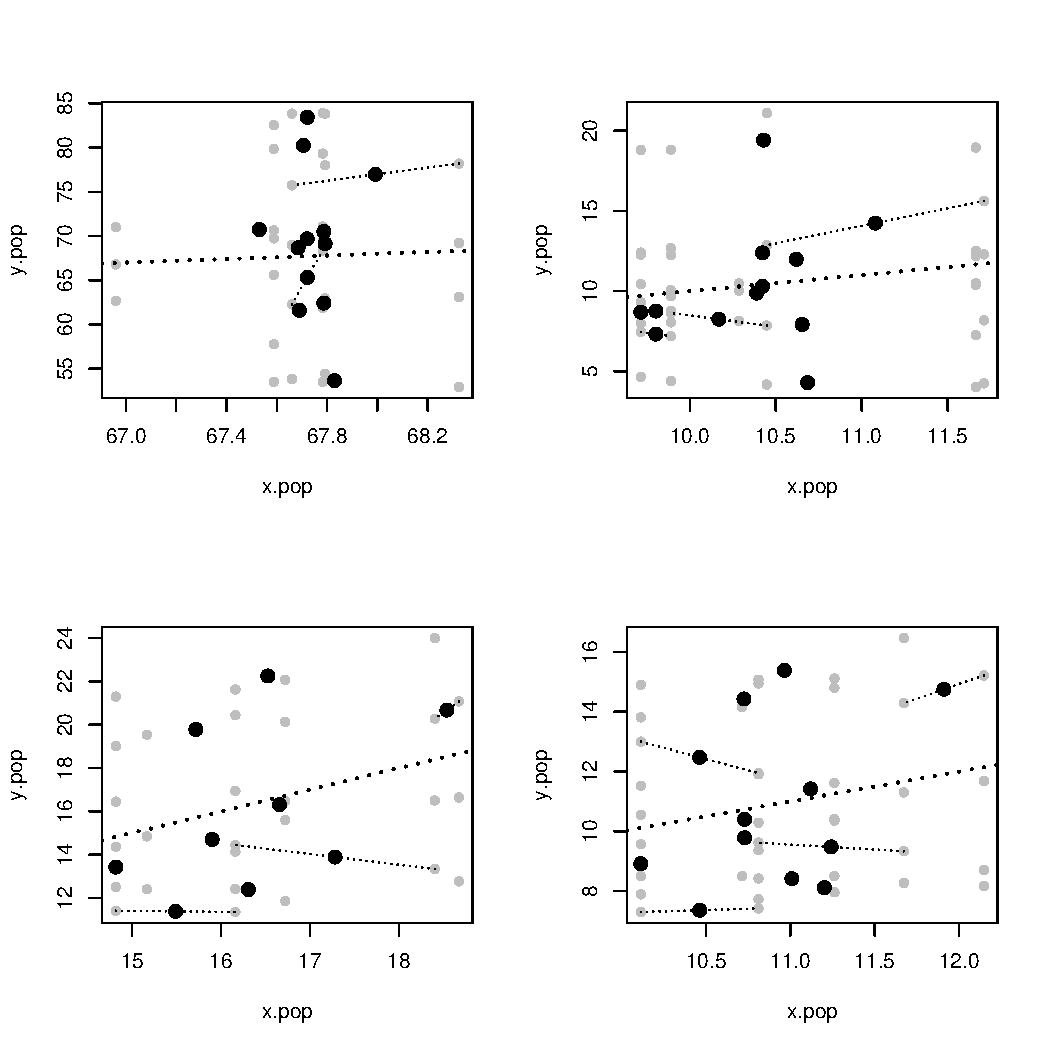
\includegraphics[width=\maxwidth]{figure/unnamed-chunk-272} 
\begin{kframe}\begin{alltt}
\hlkwd{plotSpPop}\hlstd{(traits.finch, ind.plot.finch, sp.finch,}
           \hlkwc{silent}\hlstd{=}\hlnum{TRUE}\hlstd{,} \hlkwc{resume}\hlstd{=}\hlnum{TRUE}\hlstd{,} \hlkwc{col.pop}\hlstd{=}\hlstr{"grey"}\hlstd{,} \hlkwc{col.sp}\hlstd{=}\hlstr{"black"}\hlstd{,}
           \hlkwc{p.val}\hlstd{=}\hlnum{0.1}\hlstd{,}  \hlkwc{min.ind.signif}\hlstd{=}\hlnum{3}\hlstd{)}
\end{alltt}
\end{kframe}
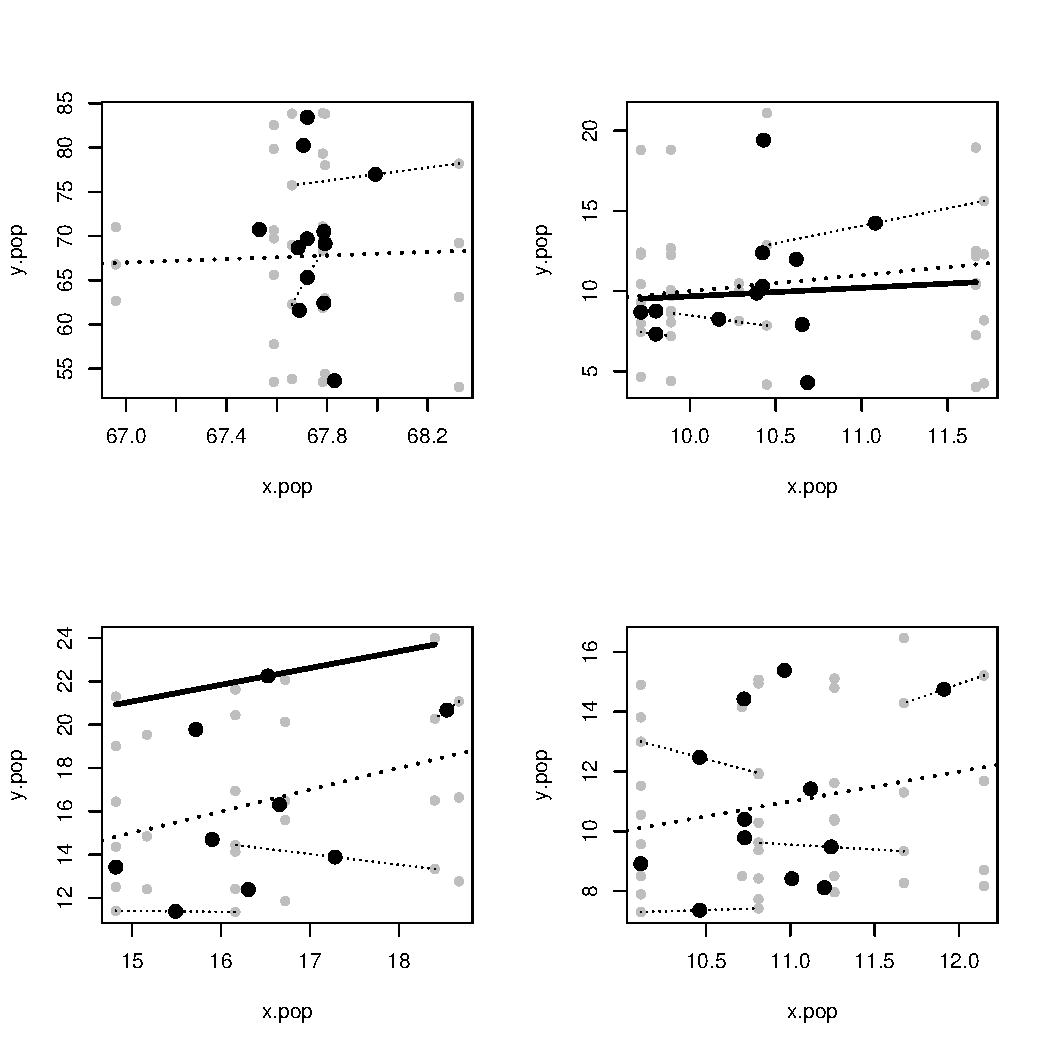
\includegraphics[width=\maxwidth]{figure/unnamed-chunk-273} 

\end{knitrout}



\newpage

%%%%%%%%%%%%%%%%
\section{Test of community assembly}
%%%%%%%%%%%%%%%%

\subsection{Ratio of variances: T-statistics}

The funcion Tstats computes observed T-statistics (T for Traits; Violle et al (2012)) as three ratios of variance, namely $T_IP/IC$, $T_IC/IR$ and $T_PC/PR$. This function can also return the distribution of these three statistics under null models.
\\

\textbf{Reference}: Violle, C., Enquist, B.J., McGill, B.J., Jiang, L., Albert, C., Hulshof, C., Jung, V. and Messier, J. (2012) The return of the variance: intraspecific variability in community ecology. Trends in Ecology and Evolution, 27, 244-252.

\begin{knitrout}
\definecolor{shadecolor}{rgb}{0.969, 0.969, 0.969}\color{fgcolor}\begin{kframe}
\begin{alltt}
\hlstd{res.finch}\hlkwb{<-}\hlkwd{Tstats}\hlstd{(traits.finch,} \hlkwc{ind.plot}\hlstd{=ind.plot.finch,} \hlkwc{sp}\hlstd{=sp.finch,}
                  \hlkwc{nperm}\hlstd{=}\hlnum{9}\hlstd{,} \hlkwc{print}\hlstd{=}\hlnum{FALSE}\hlstd{)}
\hlstd{res.finch}
\end{alltt}
\begin{verbatim}
## $Tstats
##            Length Class  Mode   
## T_IP.IC     24    -none- numeric
## T_IC.IR     24    -none- numeric
## T_PC.PR     24    -none- numeric
## T_IP.IC_nm 216    -none- numeric
## T_IC.IR_nm 216    -none- numeric
## T_PC.PR_nm 216    -none- numeric
## 
## $variances
##              Length Class  Mode   
## var_IP        156   -none- numeric
## var_PC         24   -none- numeric
## var_CR          4   -none- numeric
## var_IC         24   -none- numeric
## var_PR          4   -none- numeric
## var_IR          4   -none- numeric
## var_IP_nm1   1404   -none- numeric
## var_PC_nm2sp  216   -none- numeric
## var_IC_nm1    216   -none- numeric
## var_IC_nm2    216   -none- numeric
## var_PR_nm2sp   36   -none- numeric
## var_IR_nm2     36   -none- numeric
\end{verbatim}
\begin{alltt}
\hlkwd{attributes}\hlstd{(res.finch)}
\end{alltt}
\begin{verbatim}
## $names
## [1] "Tstats"    "variances"
## 
## $class
## [1] "Tstats"
\end{verbatim}
\begin{alltt}
\hlkwd{str}\hlstd{(res.finch)}
\end{alltt}
\begin{verbatim}
## List of 2
##  $ Tstats   :List of 6
##   ..$ T_IP.IC   : num [1:6, 1:4] 0.3831 0.0343 0.1084 0.0417 0.0496 ...
##   .. ..- attr(*, "dimnames")=List of 2
##   .. .. ..$ : chr [1:6] "DMaj" "EspHd" "FlorChrl" "GnovTwr" ...
##   .. .. ..$ : chr [1:4] "WingL" "BeakH" "UBeakL" "N.UBkL"
##   ..$ T_IC.IR   : num [1:6, 1:4] 0.0925 1.7103 0.5752 1.7916 1.3718 ...
##   .. ..- attr(*, "dimnames")=List of 2
##   .. .. ..$ : chr [1:6] "DMaj" "EspHd" "FlorChrl" "GnovTwr" ...
##   .. .. ..$ : chr [1:4] "WingL" "BeakH" "UBeakL" "N.UBkL"
##   ..$ T_PC.PR   : num [1:6, 1:4] 0.226 1.468 0.871 1.762 1.476 ...
##   .. ..- attr(*, "dimnames")=List of 2
##   .. .. ..$ : chr [1:6] "DMaj" "EspHd" "FlorChrl" "GnovTwr" ...
##   .. .. ..$ : chr [1:4] "WingL" "BeakH" "UBeakL" "N.UBkL"
##   ..$ T_IP.IC_nm: num [1:9, 1:4, 1:6] 0.948 1 3.226 2.291 2.216 ...
##   .. ..- attr(*, "dimnames")=List of 3
##   .. .. ..$ : NULL
##   .. .. ..$ : chr [1:4] "WingL" "BeakH" "UBeakL" "N.UBkL"
##   .. .. ..$ : NULL
##   ..$ T_IC.IR_nm: num [1:9, 1:4, 1:6] 0.948 1.183 0.875 1.067 1.067 ...
##   .. ..- attr(*, "dimnames")=List of 3
##   .. .. ..$ : NULL
##   .. .. ..$ : chr [1:4] "WingL" "BeakH" "UBeakL" "N.UBkL"
##   .. .. ..$ : NULL
##   ..$ T_PC.PR_nm: num [1:9, 1:4, 1:6] 0.707 0.357 5.311 7.249 4.839 ...
##   .. ..- attr(*, "dimnames")=List of 3
##   .. .. ..$ : NULL
##   .. .. ..$ : chr [1:4] "WingL" "BeakH" "UBeakL" "N.UBkL"
##   .. .. ..$ : NULL
##  $ variances:List of 12
##   ..$ var_IP      : num [1:39, 1:4] NA 4.6 4.5 2.94 3.54 ...
##   ..$ var_PC      : num [1:6, 1:4] 17.4 112.8 66.9 135.3 113.3 ...
##   ..$ var_CR      : num [1:4] 1.941 0.473 1.376 0.235
##   ..$ var_IC      : num [1:6, 1:4] 6.49 120.02 40.37 125.72 96.26 ...
##   ..$ var_PR      : num [1:4] 76.8 17.89 13.97 7.36
##   ..$ var_IR      : num [1:4] 70.17 14.01 12.49 7.52
##   ..$ var_IP_nm1  : num [1:9, 1:4, 1:39] NA NA NA NA NA NA NA NA NA NA ...
##   ..$ var_PC_nm2sp: num [1:9, 1:4, 1:6] 58.7 32.8 557.5 896.8 334.2 ...
##   ..$ var_IC_nm1  : num [1:9, 1:4, 1:6] 6.49 125.4 43.19 25.3 22.78 ...
##   ..$ var_IC_nm2  : num [1:9, 1:4, 1:6] 67.1 81.6 61.8 77.4 76.5 ...
##   ..$ var_PR_nm2sp: num [1:9, 1:4] 83.1 91.9 105 123.7 69.1 ...
##   ..$ var_IR_nm2  : num [1:9, 1:4] 70.8 69 70.6 72.5 71.8 ...
##  - attr(*, "class")= chr "Tstats"
\end{verbatim}
\end{kframe}
\end{knitrout}


\subsubsection{S3 methods for class Tstats}
Tstats class is associated to S3 methods plot, barplot, print and summary

\begin{knitrout}
\definecolor{shadecolor}{rgb}{0.969, 0.969, 0.969}\color{fgcolor}\begin{kframe}
\begin{alltt}
\hlkwd{plot}\hlstd{(res.finch)}
\hlkwd{abline}\hlstd{(}\hlkwc{v}\hlstd{=}\hlnum{0}\hlstd{)}
\end{alltt}
\end{kframe}

{\centering 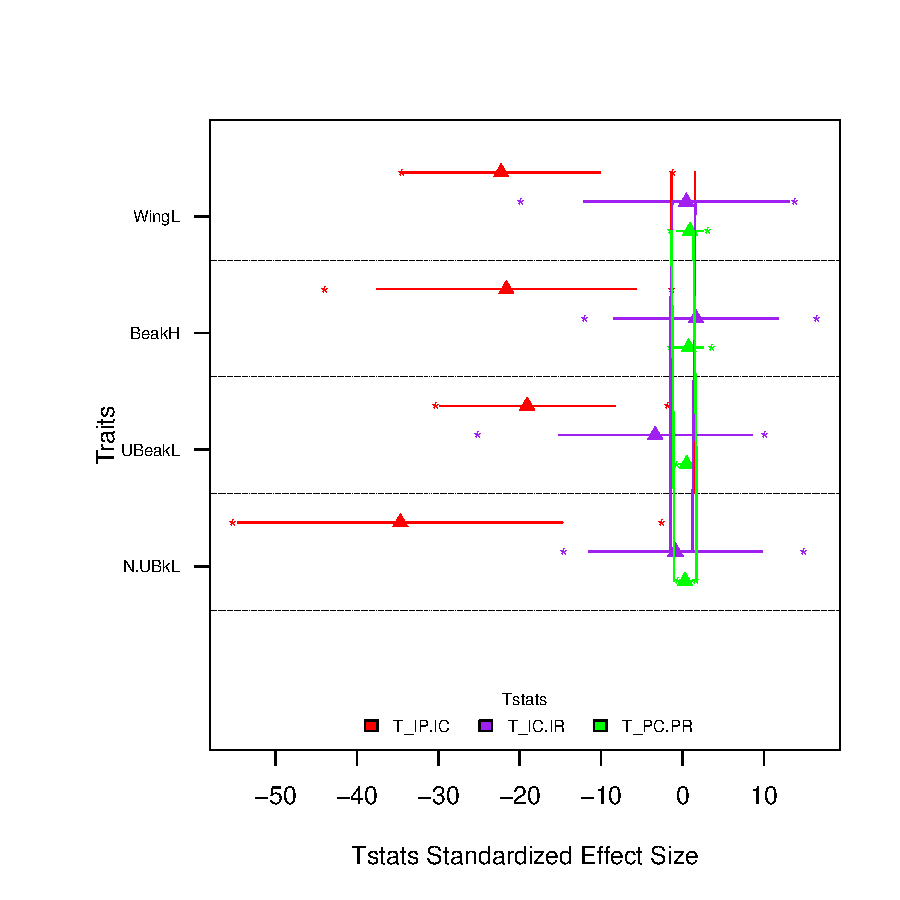
\includegraphics[width=\maxwidth]{figure/unnamed-chunk-29} 

}



\end{knitrout}

There is multiple kind of representation avaible
\begin{knitrout}
\definecolor{shadecolor}{rgb}{0.969, 0.969, 0.969}\color{fgcolor}\begin{kframe}
\begin{alltt}
\hlkwd{par}\hlstd{(}\hlkwc{mfrow}\hlstd{=}\hlkwd{c}\hlstd{(}\hlnum{2}\hlstd{,}\hlnum{2}\hlstd{))}
\hlkwd{plot}\hlstd{(res.finch,} \hlkwc{type}\hlstd{=}\hlstr{"color_cond"}\hlstd{)}
\hlkwd{plot}\hlstd{(res.finch,} \hlkwc{type}\hlstd{=}\hlstr{"simple"}\hlstd{)}
\hlkwd{plot}\hlstd{(res.finch,} \hlkwc{type}\hlstd{=}\hlstr{"simple_sd"}\hlstd{)}
\hlkwd{plot}\hlstd{(res.finch,} \hlkwc{type}\hlstd{=}\hlstr{"barplot"}\hlstd{)}
\end{alltt}
\end{kframe}

{\centering 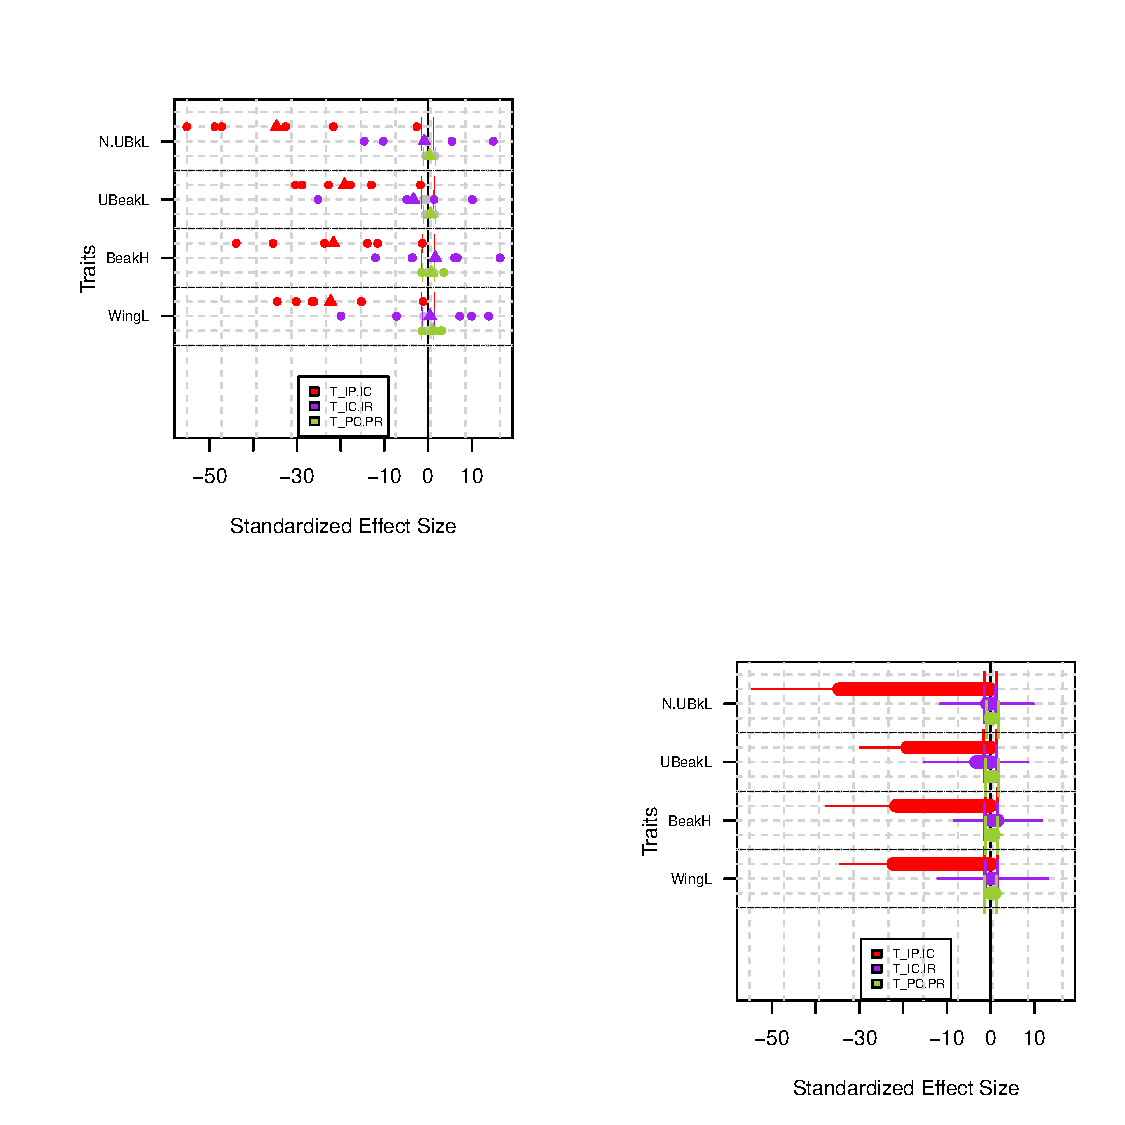
\includegraphics[width=\maxwidth]{figure/unnamed-chunk-30} 

}


\begin{kframe}\begin{alltt}
\hlkwd{par}\hlstd{(old.par)}
\end{alltt}
\end{kframe}
\end{knitrout}

\newpage

\begin{knitrout}
\definecolor{shadecolor}{rgb}{0.969, 0.969, 0.969}\color{fgcolor}\begin{kframe}
\begin{alltt}
\hlkwd{barplot}\hlstd{(res.finch,} \hlkwc{ylim}\hlstd{=}\hlkwd{c}\hlstd{(}\hlnum{0}\hlstd{,}\hlnum{3.5}\hlstd{))}
\end{alltt}
\end{kframe}

{\centering 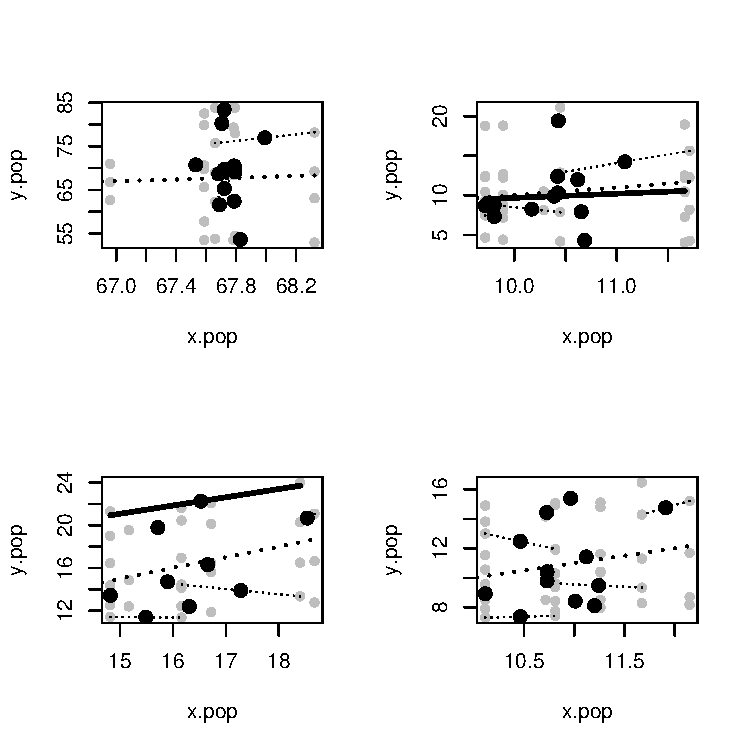
\includegraphics[width=\maxwidth]{figure/unnamed-chunk-31} 

}



\end{knitrout}

\begin{knitrout}
\definecolor{shadecolor}{rgb}{0.969, 0.969, 0.969}\color{fgcolor}\begin{kframe}
\begin{alltt}
\hlkwd{summary}\hlstd{(res.finch)} \hlcom{#S3 summary method for class Tstats}
\end{alltt}
\begin{verbatim}
## [1] "Observed values"
## $T_IP.IC
##      WingL            BeakH            UBeakL           N.UBkL      
##  Min.   :0.0343   Min.   :0.0153   Min.   :0.0267   Min.   :0.0238  
##  1st Qu.:0.0436   1st Qu.:0.0191   1st Qu.:0.0417   1st Qu.:0.0367  
##  Median :0.0645   Median :0.0400   Median :0.0544   Median :0.0403  
##  Mean   :0.1161   Mean   :0.1094   Mean   :0.0764   Mean   :0.0615  
##  3rd Qu.:0.1012   3rd Qu.:0.0580   3rd Qu.:0.0629   3rd Qu.:0.0494  
##  Max.   :0.3831   Max.   :0.4852   Max.   :0.2196   Max.   :0.1764  
## 
## $T_IC.IR
##      WingL            BeakH            UBeakL          N.UBkL     
##  Min.   :0.0925   Min.   :0.0632   Min.   :0.246   Min.   :0.257  
##  1st Qu.:0.6739   1st Qu.:0.4913   1st Qu.:0.668   1st Qu.:0.724  
##  Median :1.1707   Median :1.1831   Median :0.944   Median :0.980  
##  Mean   :1.0852   Mean   :1.1236   Mean   :0.911   Mean   :0.968  
##  3rd Qu.:1.6257   3rd Qu.:1.6242   3rd Qu.:1.080   3rd Qu.:1.314  
##  Max.   :1.7916   Max.   :2.2802   Max.   :1.629   Max.   :1.525  
## 
## $T_PC.PR
##      WingL           BeakH            UBeakL          N.UBkL     
##  Min.   :0.226   Min.   :0.0868   Min.   :0.933   Min.   :0.936  
##  1st Qu.:0.898   1st Qu.:0.8625   1st Qu.:0.983   1st Qu.:1.039  
##  Median :1.223   Median :1.0589   Median :1.125   Median :1.099  
##  Mean   :1.130   Mean   :1.2370   Mean   :1.149   Mean   :1.196  
##  3rd Qu.:1.474   3rd Qu.:1.3286   3rd Qu.:1.215   3rd Qu.:1.351  
##  Max.   :1.762   Max.   :3.0016   Max.   :1.530   Max.   :1.585  
## 
## [1] "Null values"
## $T_IP.IC_nm
##    Min. 1st Qu.  Median    Mean 3rd Qu.    Max. 
##   0.422   0.961   0.992   1.000   1.020   3.230 
## 
## $T_IC.IR_nm
##    Min. 1st Qu.  Median    Mean 3rd Qu.    Max. 
##   0.678   0.962   1.000   1.000   1.040   1.520 
## 
## $T_PC.PR_nm
##    Min. 1st Qu.  Median    Mean 3rd Qu.    Max.    NA's 
##   0.003   0.438   0.838   1.160   1.390   7.460       2
\end{verbatim}
\begin{alltt}
\hlkwd{attributes}\hlstd{(}\hlkwd{sum_Tstats}\hlstd{(res.finch))} \hlcom{#An other mean to summarize Tstatistics}
\end{alltt}
\begin{verbatim}
## $names
## [1] "p.value" "percent" "sites"   "binary"
\end{verbatim}
\begin{alltt}
\hlkwd{head}\hlstd{(}\hlkwd{sum_Tstats}\hlstd{(res.finch)}\hlopt{$}\hlstd{p.value,} \hlnum{10}\hlstd{)}
\end{alltt}
\begin{verbatim}
##             WingL BeakH UBeakL N.UBkL
## T_IP.IC.inf   0.1   0.1    0.1    0.1
## T_IP.IC.inf   0.1   0.1    0.1    0.1
## T_IP.IC.inf   0.1   0.1    0.1    0.1
## T_IP.IC.inf   0.1   0.1    0.1    0.1
## T_IP.IC.inf   0.1   0.1    0.1    0.1
## T_IP.IC.inf   0.1   0.1    0.1    0.1
## T_IP.IC.sup   1.0   1.0    1.0    1.0
## T_IP.IC.sup   1.0   1.0    1.0    1.0
## T_IP.IC.sup   1.0   1.0    1.0    1.0
## T_IP.IC.sup   1.0   1.0    1.0    1.0
\end{verbatim}
\end{kframe}
\end{knitrout}

\newpage

\subsubsection{Plot T-statistics correlations}

We can also see T-statistics correlations and theirs correlation with others variables (e.g. a gradient variable, or the species richness).

\begin{knitrout}
\definecolor{shadecolor}{rgb}{0.969, 0.969, 0.969}\color{fgcolor}\begin{kframe}
\begin{alltt}
\hlkwd{par}\hlstd{(}\hlkwc{mfrow}\hlstd{=}\hlkwd{c}\hlstd{(}\hlnum{2}\hlstd{,}\hlnum{3}\hlstd{))}
\hlkwd{plotCorTstats}\hlstd{(res.finch,} \hlkwc{plot.ask}\hlstd{=}\hlnum{FALSE}\hlstd{,} \hlkwc{multipanel}\hlstd{=F)}
\end{alltt}
\end{kframe}
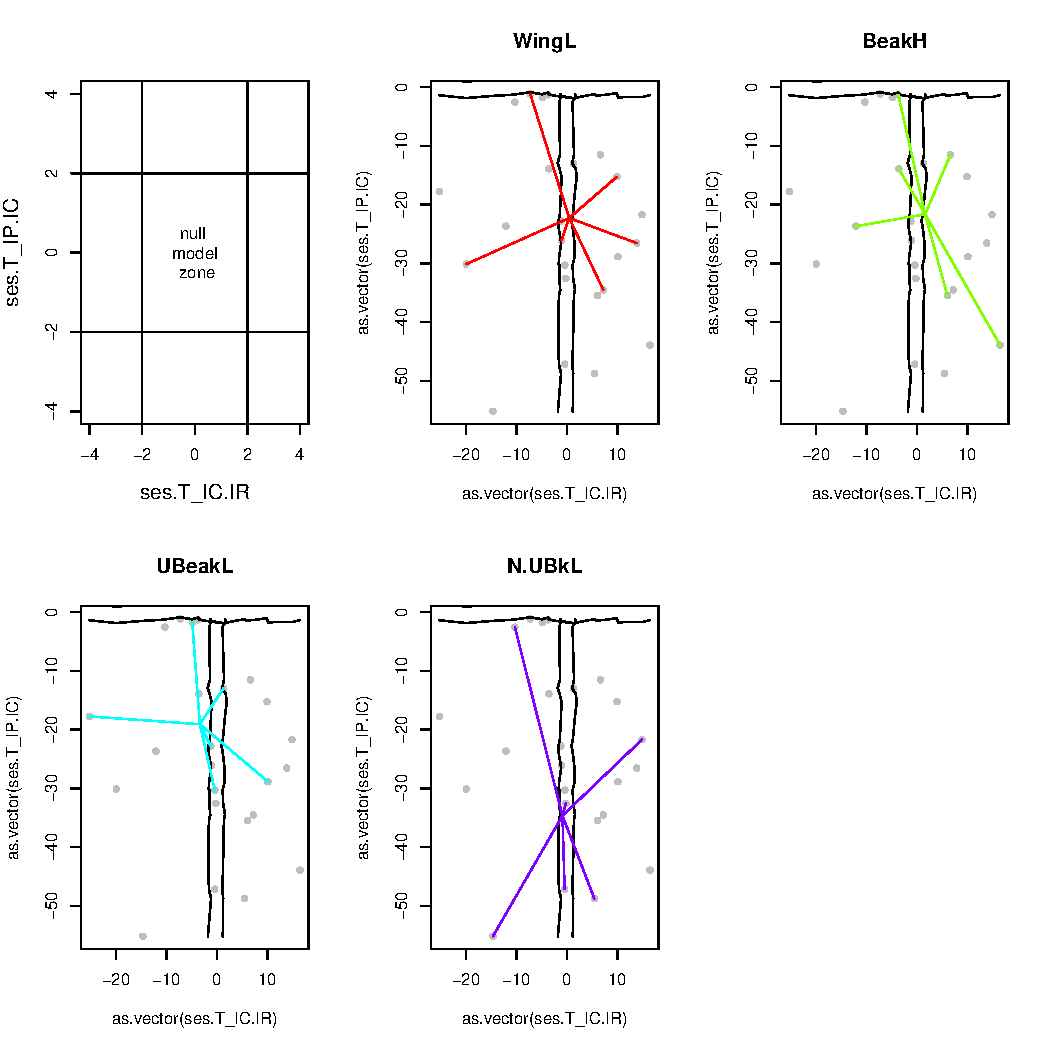
\includegraphics[width=\maxwidth]{figure/unnamed-chunk-331} 

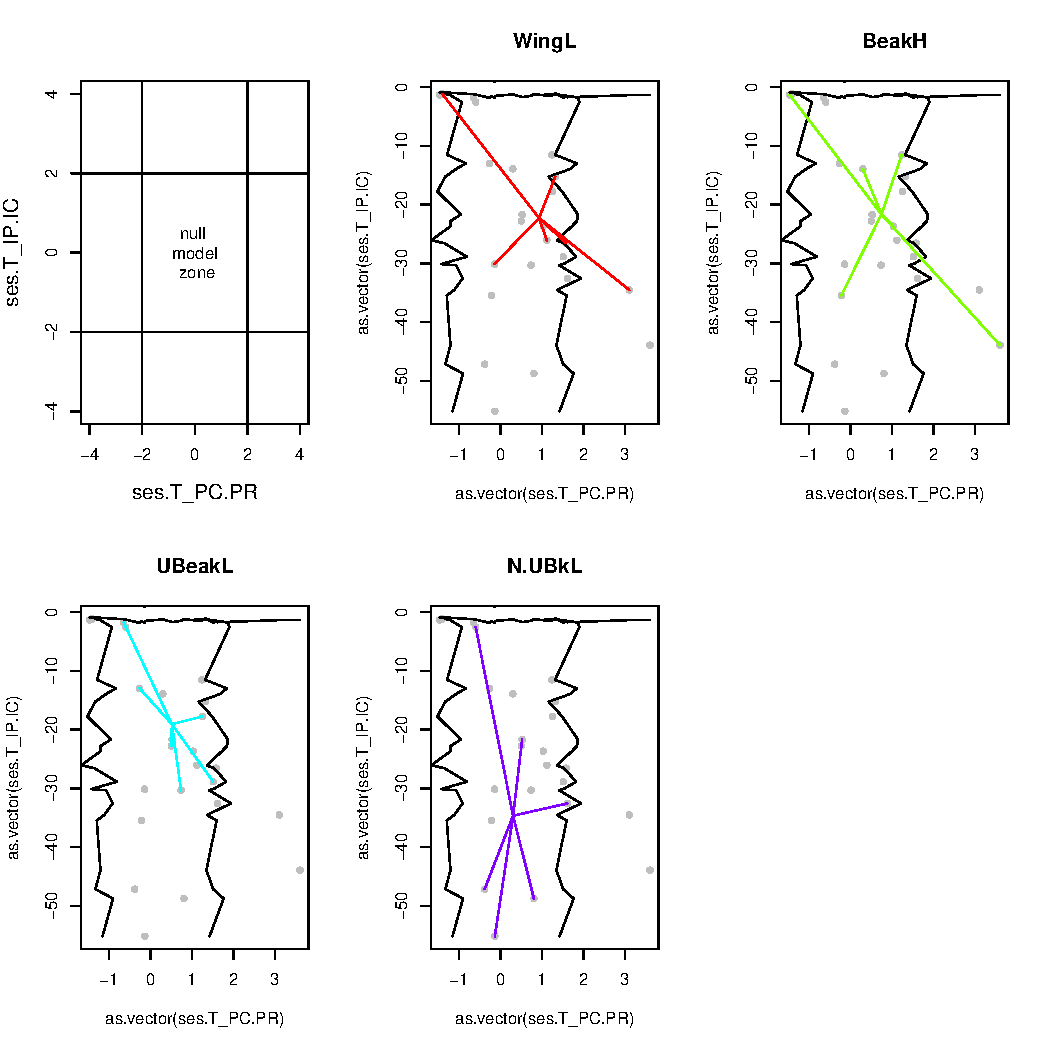
\includegraphics[width=\maxwidth]{figure/unnamed-chunk-332} 

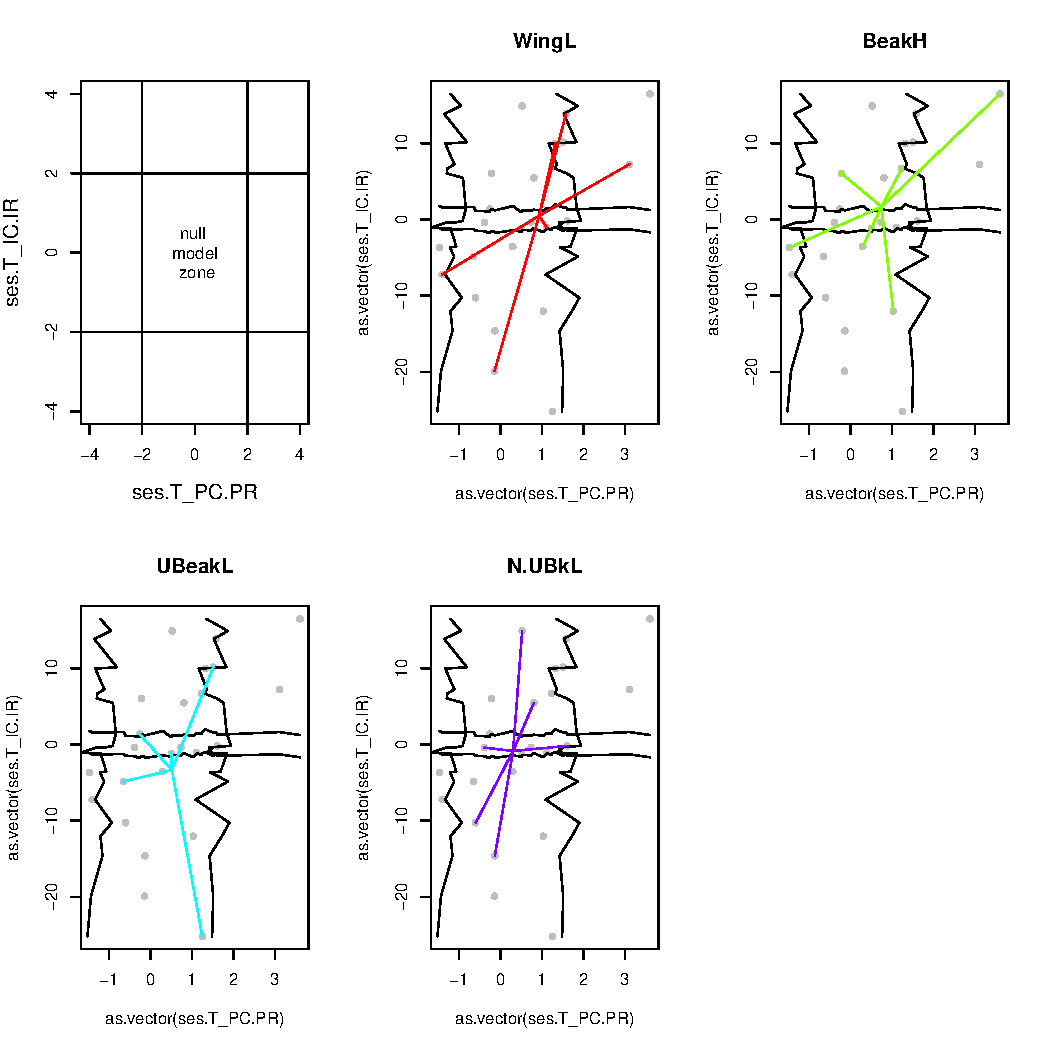
\includegraphics[width=\maxwidth]{figure/unnamed-chunk-333} 

\end{knitrout}

Here we plot T-statistics (in the standardized effect size SES form) in function of species richness by sites.

\begin{knitrout}
\definecolor{shadecolor}{rgb}{0.969, 0.969, 0.969}\color{fgcolor}\begin{kframe}
\begin{alltt}
\hlkwd{par}\hlstd{(}\hlkwc{mfrow}\hlstd{=}\hlkwd{c}\hlstd{(}\hlnum{2}\hlstd{,}\hlnum{2}\hlstd{))}
\hlstd{species.richness}\hlkwb{<-}\hlkwd{table}\hlstd{(ind.plot.finch)}
\hlkwd{plotSESvar}\hlstd{(}\hlkwd{as.listofindex}\hlstd{(}\hlkwd{list}\hlstd{(res.finch)), species.richness,}
             \hlkwc{multipanel}\hlstd{=F)}
\end{alltt}
\end{kframe}
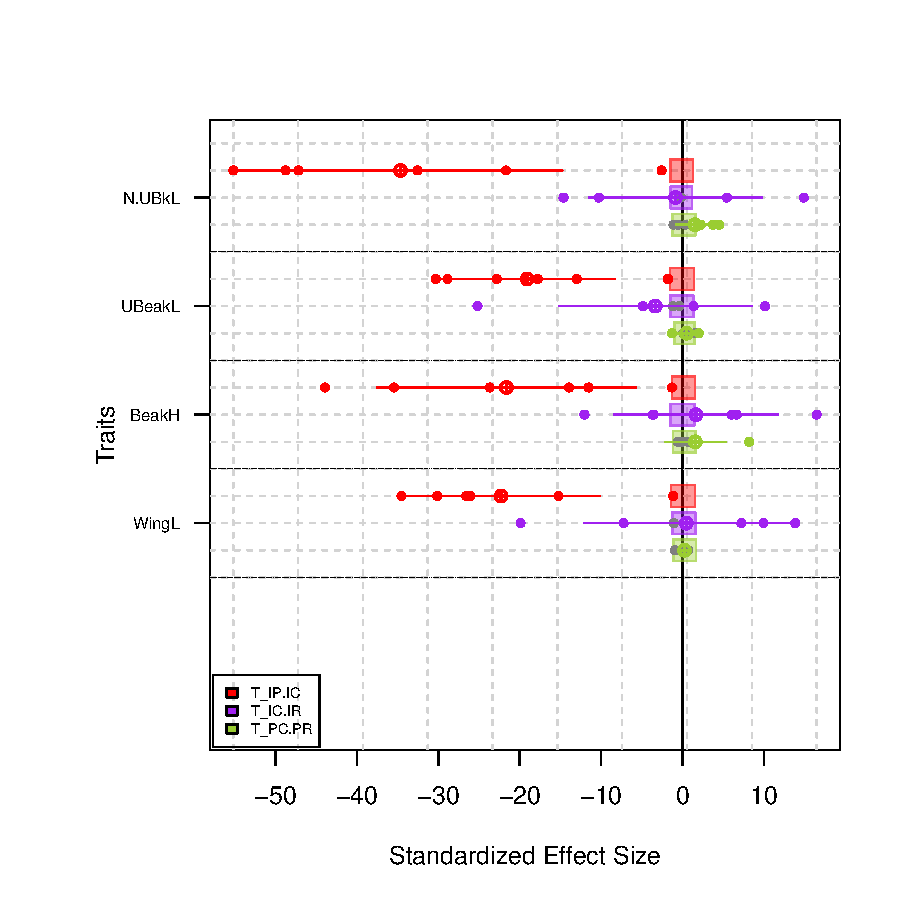
\includegraphics[width=\maxwidth]{figure/unnamed-chunk-34} 

\end{knitrout}

Same plot with \tt{resume=TRUE}.

\begin{knitrout}
\definecolor{shadecolor}{rgb}{0.969, 0.969, 0.969}\color{fgcolor}\begin{kframe}
\begin{alltt}
\hlkwd{par}\hlstd{(}\hlkwc{mfrow}\hlstd{=}\hlkwd{c}\hlstd{(}\hlnum{2}\hlstd{,}\hlnum{2}\hlstd{))}
\hlkwd{plotSESvar}\hlstd{(}\hlkwd{as.listofindex}\hlstd{(}\hlkwd{list}\hlstd{(res.finch)), species.richness,}
             \hlkwc{resume}\hlstd{=T,} \hlkwc{multipanel}\hlstd{=F)}
\end{alltt}
\end{kframe}
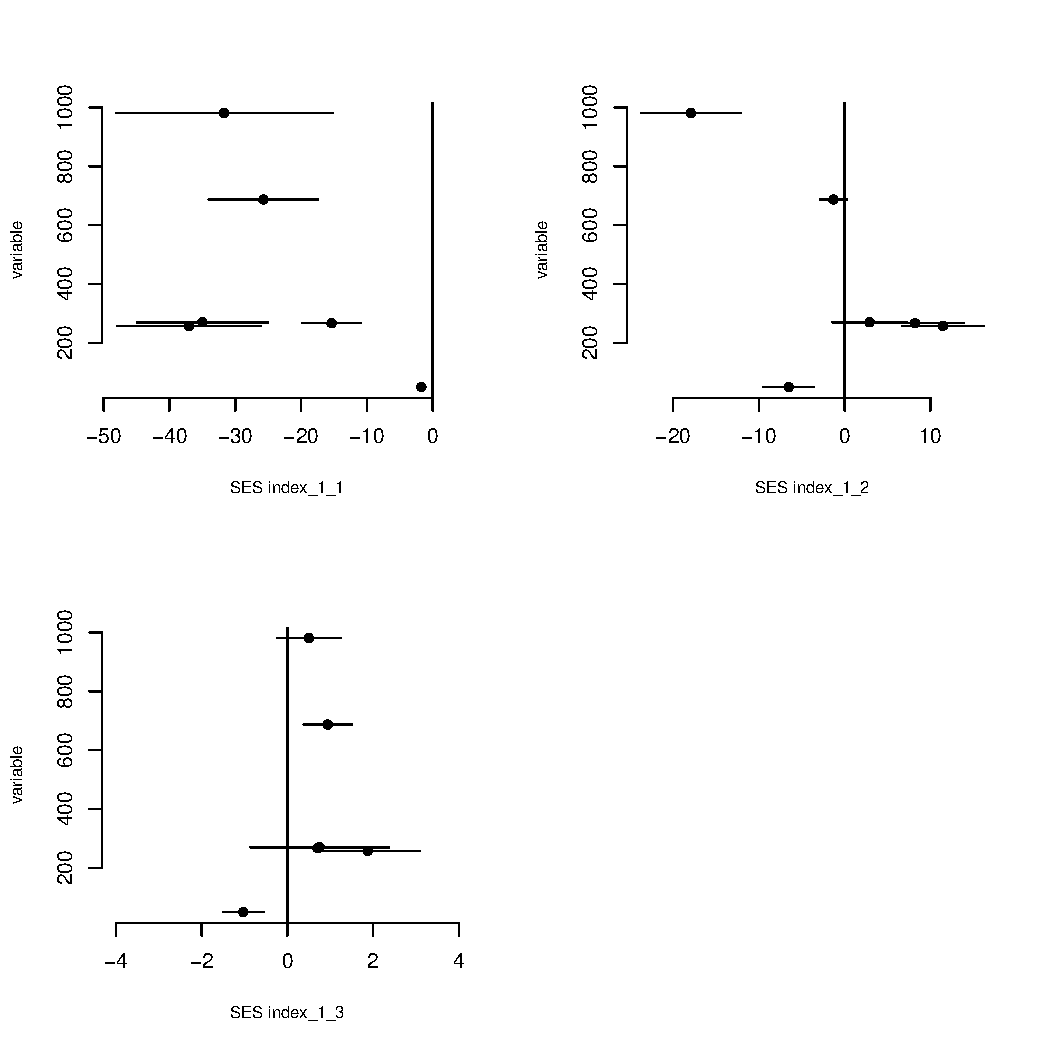
\includegraphics[width=\maxwidth]{figure/unnamed-chunk-35} 
\begin{kframe}\begin{alltt}
\hlkwd{par}\hlstd{(}\hlkwc{mfrow}\hlstd{=}\hlkwd{c}\hlstd{(}\hlnum{1}\hlstd{,}\hlnum{1}\hlstd{))}
\end{alltt}
\end{kframe}
\end{knitrout}


\newpage
\subsection{Others univariates metrics: function \tt{ComIndex} and \tt{ComIndexMulti}}

The function \tt{ComIndex} allow to choose your own function (like mean, range, variance...) to calculate customize metrics. Here CVNND refers to the Coefficient of Variation of the Nearest Neighborhood Distance. ComIndexMulti do the same things for multivariate metrics. 

\begin{knitrout}
\definecolor{shadecolor}{rgb}{0.969, 0.969, 0.969}\color{fgcolor}\begin{kframe}
\begin{alltt}
\hlcom{#Define the funcions to calculate}
\hlstd{funct}\hlkwb{<-}\hlkwd{c}\hlstd{(}\hlstr{"mean(x, na.rm=T)"}\hlstd{,} \hlstr{"kurtosis(x, na.rm=T)"}\hlstd{,}
         \hlstr{"max(x, na.rm=T) - min(x, na.rm=T)"}\hlstd{,} \hlstr{"CVNND(x)"}  \hlstd{)}

\hlcom{#Test against the null model 2}
\hlstd{res.finch.sp_mn2}\hlkwb{<-}\hlkwd{ComIndex}\hlstd{(}\hlkwc{traits}\hlstd{=traits.finch,} \hlkwc{index}\hlstd{=funct,} \hlkwc{sp}\hlstd{=sp.finch,}
                           \hlkwc{nullmodels}\hlstd{=}\hlkwd{c}\hlstd{(}\hlnum{2}\hlstd{,}\hlnum{2}\hlstd{,}\hlnum{2}\hlstd{,}\hlnum{2}\hlstd{),} \hlkwc{ind.plot}\hlstd{=ind.plot.finch,}
                           \hlkwc{nperm}\hlstd{=}\hlnum{9}\hlstd{,} \hlkwc{print}\hlstd{=}\hlnum{FALSE}\hlstd{)}

\hlcom{#Test against the null model 2sp}
\hlstd{res.finch.sp_mn2sp}\hlkwb{<-}\hlkwd{ComIndex}\hlstd{(}\hlkwc{traits}\hlstd{=traits.finch,} \hlkwc{index}\hlstd{=funct,} \hlkwc{sp}\hlstd{=sp.finch,}
                             \hlkwc{nullmodels}\hlstd{=}\hlkwd{rep}\hlstd{(}\hlstr{"2sp"}\hlstd{,}\hlnum{4}\hlstd{),} \hlkwc{ind.plot}\hlstd{=ind.plot.finch,}
                             \hlkwc{nperm}\hlstd{=}\hlnum{9}\hlstd{,} \hlkwc{print}\hlstd{=}\hlnum{FALSE}\hlstd{)}
\end{alltt}
\end{kframe}
\end{knitrout}

These two functions allows to calcul index by sites for example using \code{"tapply(x, sites, mean)"}.

\begin{knitrout}
\definecolor{shadecolor}{rgb}{0.969, 0.969, 0.969}\color{fgcolor}\begin{kframe}
\begin{alltt}
\hlstd{funct}\hlkwb{<-}\hlkwd{c}\hlstd{(}\hlstr{"tapply(x, ind.plot.finch, function(x) mean(x, na.rm=T))"}\hlstd{,}
         \hlstr{"tapply(x, ind.plot.finch, function(x) kurtosis(x, na.rm=T))"}\hlstd{,}
         \hlstr{"tapply(x, ind.plot.finch, function(x) max(x, na.rm=T)-min(x, na.rm=T))"}\hlstd{,}
         \hlstr{"tapply(x, ind.plot.finch, function(x) CVNND(x))"}  \hlstd{)}

\hlcom{##Null model 1 is trivial for this function}
\hlcom{##because randomisation is within community only}

\hlstd{res.finch.ind_mn1}\hlkwb{<-}\hlkwd{ComIndex}\hlstd{(}\hlkwc{traits}\hlstd{=traits.finch,} \hlkwc{index}\hlstd{=funct,} \hlkwc{sp}\hlstd{=sp.finch,}
                             \hlkwc{nullmodels}\hlstd{=}\hlkwd{c}\hlstd{(}\hlnum{1}\hlstd{,}\hlnum{1}\hlstd{,}\hlnum{1}\hlstd{,}\hlnum{1}\hlstd{),} \hlkwc{ind.plot}\hlstd{=ind.plot.finch,}
                             \hlkwc{nperm}\hlstd{=}\hlnum{9}\hlstd{,} \hlkwc{print}\hlstd{=}\hlnum{FALSE}\hlstd{)}
\hlstd{res.finch.ind_mn2}\hlkwb{<-}\hlkwd{ComIndex}\hlstd{(}\hlkwc{traits}\hlstd{=traits.finch,} \hlkwc{index}\hlstd{=funct,} \hlkwc{sp}\hlstd{=sp.finch,}
                             \hlkwc{nullmodels}\hlstd{=}\hlkwd{c}\hlstd{(}\hlnum{2}\hlstd{,}\hlnum{2}\hlstd{,}\hlnum{2}\hlstd{,}\hlnum{2}\hlstd{),} \hlkwc{ind.plot}\hlstd{=ind.plot.finch,}
                             \hlkwc{nperm}\hlstd{=}\hlnum{9}\hlstd{,} \hlkwc{print}\hlstd{=}\hlnum{FALSE}\hlstd{)}
\end{alltt}
\end{kframe}
\end{knitrout}


We can calcul index with or without intraspecific variance.

\begin{knitrout}
\definecolor{shadecolor}{rgb}{0.969, 0.969, 0.969}\color{fgcolor}\begin{kframe}
\begin{alltt}
\hlcom{#Calcul of means by population (name_sp_site is a name of a population) }
\hlcom{#like in the function ComIndex and determine the site for each population (sites_bypop)}

\hlstd{name_sp_sites}\hlkwb{=}\hlkwd{paste}\hlstd{(sp.finch, ind.plot.finch,}\hlkwc{sep}\hlstd{=}\hlstr{"_"}\hlstd{)}
\hlstd{traits.by.pop}\hlkwb{<-}\hlkwd{apply}\hlstd{(traits.finch,} \hlnum{2} \hlstd{,}
                     \hlkwa{function} \hlstd{(}\hlkwc{x}\hlstd{)} \hlkwd{tapply}\hlstd{(x, name_sp_sites, mean ,} \hlkwc{na.rm}\hlstd{=T))}

\hlstd{sites_bypop}\hlkwb{<-}\hlkwd{lapply}\hlstd{(}\hlkwd{strsplit}\hlstd{(}\hlkwd{paste}\hlstd{(}\hlkwd{rownames}\hlstd{(traits.by.pop),} \hlkwc{sep}\hlstd{=}\hlstr{"_"}\hlstd{),} \hlkwc{split}\hlstd{=}\hlstr{"_"}\hlstd{),}
                    \hlkwa{function}\hlstd{(}\hlkwc{x}\hlstd{) x[}\hlnum{3}\hlstd{])}

\hlcom{#We use the precedent list of function "funct"}
\hlstd{funct.withIV}\hlkwb{<-}\hlstd{funct}

\hlstd{fact}\hlkwb{<-}\hlkwd{unlist}\hlstd{(sites_bypop)}
\hlstd{funct.withoutIV}\hlkwb{<-}\hlkwd{c}\hlstd{(}\hlstr{"tapply(x, fact, function(x) mean(x, na.rm=T))"}\hlstd{,}
                   \hlstr{"tapply(x, fact, function(x) kurtosis(x, na.rm=T))"}\hlstd{,}
                   \hlstr{"tapply(x, fact, function(x) max(x, na.rm=T)-min(x, na.rm=T))"}\hlstd{,}
                   \hlstr{"tapply(x, fact, function(x) CVNND(x))"}\hlstd{)}


\hlstd{res.finch.withIV}\hlkwb{<-}\hlkwd{ComIndex}\hlstd{(}\hlkwc{traits}\hlstd{=traits.finch,} \hlkwc{index}\hlstd{=funct.withIV,}
                             \hlkwc{sp}\hlstd{=sp.finch,} \hlkwc{nullmodels}\hlstd{=}\hlkwd{c}\hlstd{(}\hlnum{2}\hlstd{,}\hlnum{2}\hlstd{,}\hlnum{2}\hlstd{,}\hlnum{2}\hlstd{),}
                             \hlkwc{ind.plot}\hlstd{=ind.plot.finch,} \hlkwc{nperm}\hlstd{=}\hlnum{9}\hlstd{,} \hlkwc{print}\hlstd{=}\hlnum{FALSE}\hlstd{)}

\hlstd{res.finch.withoutIV}\hlkwb{<-}\hlkwd{ComIndex}\hlstd{(}\hlkwc{traits}\hlstd{=traits.finch,} \hlkwc{index}\hlstd{=funct.withoutIV,}
                             \hlkwc{sp}\hlstd{=sp.finch,} \hlkwc{nullmodels}\hlstd{=}\hlkwd{rep}\hlstd{(}\hlstr{"2sp"}\hlstd{,}\hlnum{4}\hlstd{),}
                             \hlkwc{ind.plot}\hlstd{=ind.plot.finch,} \hlkwc{nperm}\hlstd{=}\hlnum{9}\hlstd{,} \hlkwc{print}\hlstd{=}\hlnum{FALSE}\hlstd{)}
\end{alltt}
\end{kframe}
\end{knitrout}



\subsubsection{S3 methods for class ComIndex and ComIndexMulti}
Tstats class is associated to S3 methods plot, print and summary

\begin{knitrout}
\definecolor{shadecolor}{rgb}{0.969, 0.969, 0.969}\color{fgcolor}\begin{kframe}
\begin{alltt}
\hlstd{res.finch.withIV}
\end{alltt}
\begin{verbatim}
## List of 1
##  $ obs:List of 4
##   ..$ tapply(x, ind.plot.finch, function(x) mean(x, na.rm=T))               : num [1:6, 1:4] NULL ...
##   .. ..- attr(*, "dimnames")=List of 2
##   ..$ tapply(x, ind.plot.finch, function(x) kurtosis(x, na.rm=T))           : num [1:6, 1:4] NULL ...
##   .. ..- attr(*, "dimnames")=List of 2
##   ..$ tapply(x, ind.plot.finch, function(x) max(x, na.rm=T)-min(x, na.rm=T)): num [1:6, 1:4] NULL ...
##   .. ..- attr(*, "dimnames")=List of 2
##   ..$ tapply(x, ind.plot.finch, function(x) CVNND(x))                       : num [1:6, 1:4] NULL ...
##   .. ..- attr(*, "dimnames")=List of 2
## NULL
## List of 5
##  $ Null          :List of 4
##  $ list.index    :List of 8
##  $ list.index.t  :List of 8
##  $ sites_richness: Named num [1:6] NULL ...
##   ..- attr(*, "names")= chr [1:6]  ...
##  $ namestraits   : chr [1:4]  ...
## NULL
\end{verbatim}
\begin{alltt}
\hlkwd{summary}\hlstd{(res.finch.withIV)}
\end{alltt}
\begin{verbatim}
## [1] "Observed values"
## $`tapply(x, ind.plot.finch, function(x) mean(x, na.rm=T))`
##      WingL          BeakH           UBeakL         N.UBkL    
##  Min.   :67.0   Min.   : 9.71   Min.   :14.8   Min.   :10.1  
##  1st Qu.:67.6   1st Qu.: 9.99   1st Qu.:15.4   1st Qu.:10.7  
##  Median :67.7   Median :10.37   Median :16.4   Median :11.0  
##  Mean   :67.7   Mean   :10.62   Mean   :16.7   Mean   :11.1  
##  3rd Qu.:67.8   3rd Qu.:11.36   3rd Qu.:18.0   3rd Qu.:11.6  
##  Max.   :68.3   Max.   :11.71   Max.   :18.7   Max.   :12.1  
## 
## $`tapply(x, ind.plot.finch, function(x) kurtosis(x, na.rm=T))`
##      WingL            BeakH            UBeakL           N.UBkL      
##  Min.   :-1.466   Min.   :-1.360   Min.   :-1.600   Min.   :-1.752  
##  1st Qu.:-1.252   1st Qu.:-0.642   1st Qu.:-1.185   1st Qu.:-1.449  
##  Median :-0.821   Median :-0.297   Median :-1.089   Median :-1.083  
##  Mean   :-0.622   Mean   :-0.110   Mean   :-0.564   Mean   :-0.740  
##  3rd Qu.:-0.274   3rd Qu.: 0.646   3rd Qu.:-0.876   3rd Qu.:-0.946  
##  Max.   : 0.865   Max.   : 1.087   Max.   : 2.414   Max.   : 1.950  
## 
## $`tapply(x, ind.plot.finch, function(x) max(x, na.rm=T)-min(x, na.rm=T))`
##      WingL          BeakH          UBeakL         N.UBkL     
##  Min.   :11.0   Min.   : 4.3   Min.   : 8.7   Min.   : 6.50  
##  1st Qu.:34.2   1st Qu.:14.6   1st Qu.:11.1   1st Qu.: 8.88  
##  Median :35.5   Median :16.1   Median :12.6   Median :10.05  
##  Mean   :31.8   Mean   :14.7   Mean   :11.9   Mean   : 9.33  
##  3rd Qu.:36.8   3rd Qu.:17.5   3rd Qu.:13.2   3rd Qu.:10.32  
##  Max.   :38.0   Max.   :19.4   Max.   :13.6   Max.   :10.50  
## 
## $`tapply(x, ind.plot.finch, function(x) CVNND(x))`
##      WingL          BeakH          UBeakL         N.UBkL    
##  Min.   :2.09   Min.   :1.66   Min.   :1.77   Min.   :1.89  
##  1st Qu.:2.62   1st Qu.:3.00   1st Qu.:2.17   1st Qu.:2.17  
##  Median :2.67   Median :3.27   Median :2.74   Median :2.61  
##  Mean   :3.21   Mean   :3.37   Mean   :2.61   Mean   :2.64  
##  3rd Qu.:3.73   3rd Qu.:3.47   3rd Qu.:2.91   3rd Qu.:3.10  
##  Max.   :5.17   Max.   :5.58   Max.   :3.46   Max.   :3.41  
## 
## [1] "Null values"
## $`tapply(x, ind.plot.finch, function(x) mean(x, na.rm=T))`
##    Min. 1st Qu.  Median    Mean 3rd Qu.    Max. 
##    9.66   10.60   13.30   26.20   29.20   70.30 
## 
## $`tapply(x, ind.plot.finch, function(x) kurtosis(x, na.rm=T))`
##    Min. 1st Qu.  Median    Mean 3rd Qu.    Max. 
##  -1.360  -0.951  -0.653  -0.445  -0.176   1.590 
## 
## $`tapply(x, ind.plot.finch, function(x) max(x, na.rm=T)-min(x, na.rm=T))`
##    Min. 1st Qu.  Median    Mean 3rd Qu.    Max. 
##     8.7    11.4    15.9    19.8    20.8    39.0 
## 
## $`tapply(x, ind.plot.finch, function(x) CVNND(x))`
##    Min. 1st Qu.  Median    Mean 3rd Qu.    Max. 
##   0.796   1.610   2.180   2.300   2.680   4.990
\end{verbatim}
\begin{alltt}
\hlkwd{summary}\hlstd{(res.finch.withoutIV)}
\end{alltt}
\begin{verbatim}
## [1] "Observed values"
## $`tapply(x, fact, function(x) mean(x, na.rm=T))`
##      WingL          BeakH           UBeakL         N.UBkL    
##  Min.   :65.9   Min.   : 9.55   Min.   :15.5   Min.   :10.6  
##  1st Qu.:67.2   1st Qu.:10.06   1st Qu.:15.7   1st Qu.:10.7  
##  Median :68.7   Median :10.15   Median :16.4   Median :11.0  
##  Mean   :68.1   Mean   :10.37   Mean   :16.6   Mean   :11.1  
##  3rd Qu.:69.1   3rd Qu.:10.68   3rd Qu.:17.1   3rd Qu.:11.2  
##  Max.   :69.2   Max.   :11.50   Max.   :18.5   Max.   :11.9  
## 
## $`tapply(x, fact, function(x) kurtosis(x, na.rm=T))`
##      WingL            BeakH             UBeakL          N.UBkL     
##  Min.   :-2.333   Min.   :-2.3333   Min.   :-2.33   Min.   :-2.33  
##  1st Qu.:-1.954   1st Qu.:-2.0761   1st Qu.:-2.27   1st Qu.:-2.04  
##  Median :-1.760   Median :-1.4834   Median :-1.98   Median :-1.87  
##  Mean   :-1.559   Mean   :-1.2609   Mean   :-1.99   Mean   :-1.84  
##  3rd Qu.:-1.033   3rd Qu.:-0.4232   3rd Qu.:-1.77   3rd Qu.:-1.60  
##  Max.   :-0.693   Max.   : 0.0779   Max.   :-1.60   Max.   :-1.37  
## 
## $`tapply(x, fact, function(x) max(x, na.rm=T)-min(x, na.rm=T))`
##      WingL           BeakH           UBeakL          N.UBkL    
##  Min.   : 8.33   Min.   : 2.35   Min.   : 7.14   Min.   :5.66  
##  1st Qu.:26.21   1st Qu.:12.08   1st Qu.: 8.71   1st Qu.:7.07  
##  Median :29.21   Median :14.29   Median :10.06   Median :7.38  
##  Mean   :25.41   Mean   :12.36   Mean   : 9.42   Mean   :7.22  
##  3rd Qu.:29.87   3rd Qu.:14.81   3rd Qu.:10.26   3rd Qu.:7.64  
##  Max.   :30.41   Max.   :16.93   Max.   :10.67   Max.   :8.20  
## 
## $`tapply(x, fact, function(x) CVNND(x))`
##      WingL            BeakH           UBeakL           N.UBkL     
##  Min.   :0.0162   Min.   :0.106   Min.   :0.0954   Min.   :0.382  
##  1st Qu.:0.1530   1st Qu.:0.530   1st Qu.:0.1835   1st Qu.:0.398  
##  Median :0.4492   Median :0.910   Median :0.4489   Median :0.556  
##  Mean   :0.5157   Mean   :0.784   Mean   :0.3828   Mean   :0.663  
##  3rd Qu.:0.9333   3rd Qu.:1.108   3rd Qu.:0.5212   3rd Qu.:0.909  
##  Max.   :1.0306   Max.   :1.198   Max.   :0.6635   Max.   :1.110  
## 
## [1] "Null values"
## $`tapply(x, fact, function(x) mean(x, na.rm=T))`
##    Min. 1st Qu.  Median    Mean 3rd Qu.    Max. 
##    15.6    24.7    26.7    27.0    28.6    40.3 
## 
## $`tapply(x, fact, function(x) kurtosis(x, na.rm=T))`
##    Min. 1st Qu.  Median    Mean 3rd Qu.    Max. 
##  -2.380  -2.000  -1.420  -1.200  -0.856   3.270 
## 
## $`tapply(x, fact, function(x) max(x, na.rm=T)-min(x, na.rm=T))`
##    Min. 1st Qu.  Median    Mean 3rd Qu.    Max. 
##    1.98   10.00   14.10   18.90   21.40   75.30 
## 
## $`tapply(x, fact, function(x) CVNND(x))`
##    Min. 1st Qu.  Median    Mean 3rd Qu.    Max. 
##  0.0199  0.6750  0.9220  0.9960  1.2400  2.4500
\end{verbatim}
\begin{alltt}
\hlkwd{plot}\hlstd{(res.finch.withIV)}
\end{alltt}
\end{kframe}
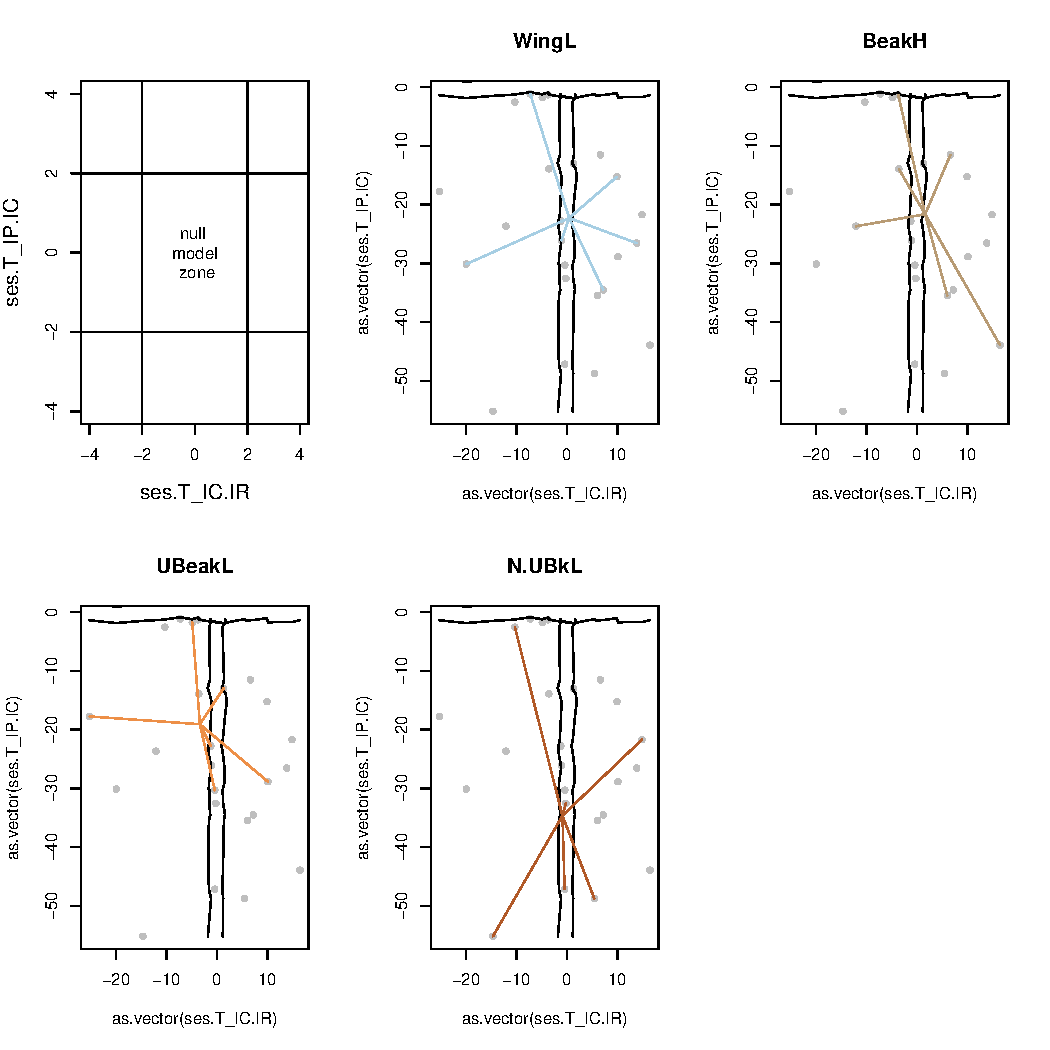
\includegraphics[width=\maxwidth]{figure/unnamed-chunk-391} 
\begin{kframe}\begin{alltt}
\hlkwd{plot}\hlstd{(res.finch.withoutIV)}
\end{alltt}
\end{kframe}
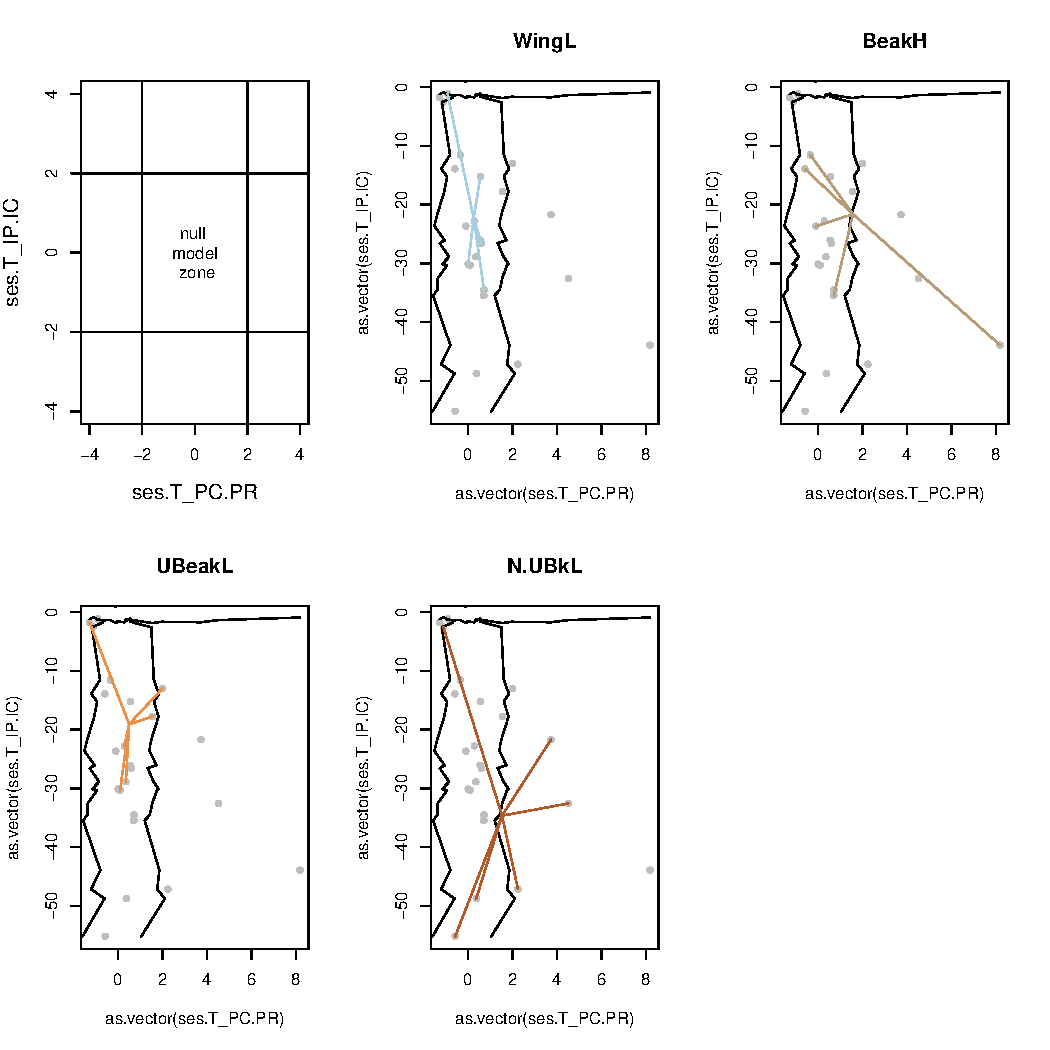
\includegraphics[width=\maxwidth]{figure/unnamed-chunk-392} 

\end{knitrout}


\subsubsection{Plot Tstats and other uni/multivariates metrics together}
The class listofindex permit to stock differents metrics computed using Tstats, ComIndex and ComIndexMulti and compared to different null model. To do that we can use the Standardized Effect Size (ses) define as : 

\begin{center}
$SES = (I_obs – I_sim) / \delta_{sim}$
\end{center}

where $I_obs$ is the observed value, $I_sim$ the mean of values calculated from the null model and $\delta_{sim}$ the standard deviation of these simulated values.


\begin{knitrout}
\definecolor{shadecolor}{rgb}{0.969, 0.969, 0.969}\color{fgcolor}\begin{kframe}
\begin{alltt}
\hlstd{list.ind1}\hlkwb{<-}\hlkwd{list}\hlstd{(res.finch.withIV, res.finch.withoutIV)}
\hlstd{index.list1}\hlkwb{<-}\hlkwd{as.listofindex}\hlstd{(list.ind1)}

\hlkwd{plot}\hlstd{(index.list1)}
\end{alltt}
\end{kframe}
\end{knitrout}

\begin{knitrout}
\definecolor{shadecolor}{rgb}{0.969, 0.969, 0.969}\color{fgcolor}\begin{kframe}
\begin{alltt}
\hlstd{list.ind}\hlkwb{<-}\hlkwd{list}\hlstd{(res.finch.withIV, res.finch.withoutIV, res.finch)}
\hlstd{namesindex.i.l1}\hlkwb{=}\hlkwd{c}\hlstd{(}\hlstr{"mean"}\hlstd{,} \hlstr{"kurtosis"}\hlstd{,} \hlstr{"range"}\hlstd{,} \hlstr{"CVNND"}\hlstd{,}
                  \hlstr{"mean.pop"}\hlstd{,} \hlstr{"kurtosis.pop"}\hlstd{,} \hlstr{"range.pop"}\hlstd{,} \hlstr{"CVNND.pop"}\hlstd{,}
                  \hlstr{"T_IP.IC"}\hlstd{,} \hlstr{"T_IC.IR"}\hlstd{,} \hlstr{"T_PC.PR"}\hlstd{)}

\hlstd{i.l1}\hlkwb{<-}\hlkwd{as.listofindex}\hlstd{(list.ind,} \hlkwc{namesindex}\hlstd{=namesindex.i.l1)}

\hlkwd{class}\hlstd{(i.l1)}
\end{alltt}
\begin{verbatim}
## [1] "listofindex"
\end{verbatim}
\end{kframe}
\end{knitrout}

The plot type \tt{bytraits} allows to plot all SES traits values for all sites or all traits
\begin{knitrout}
\definecolor{shadecolor}{rgb}{0.969, 0.969, 0.969}\color{fgcolor}\begin{kframe}
\begin{alltt}
\hlkwd{par}\hlstd{(}\hlkwc{mfrow}\hlstd{=}\hlkwd{c}\hlstd{(}\hlnum{2}\hlstd{,}\hlnum{3}\hlstd{))}
\hlkwd{plot}\hlstd{(i.l1,}\hlkwc{type}\hlstd{=}\hlstr{"bytraits"}\hlstd{,} \hlkwc{bysite}\hlstd{=}\hlnum{TRUE}\hlstd{)}
\end{alltt}
\end{kframe}
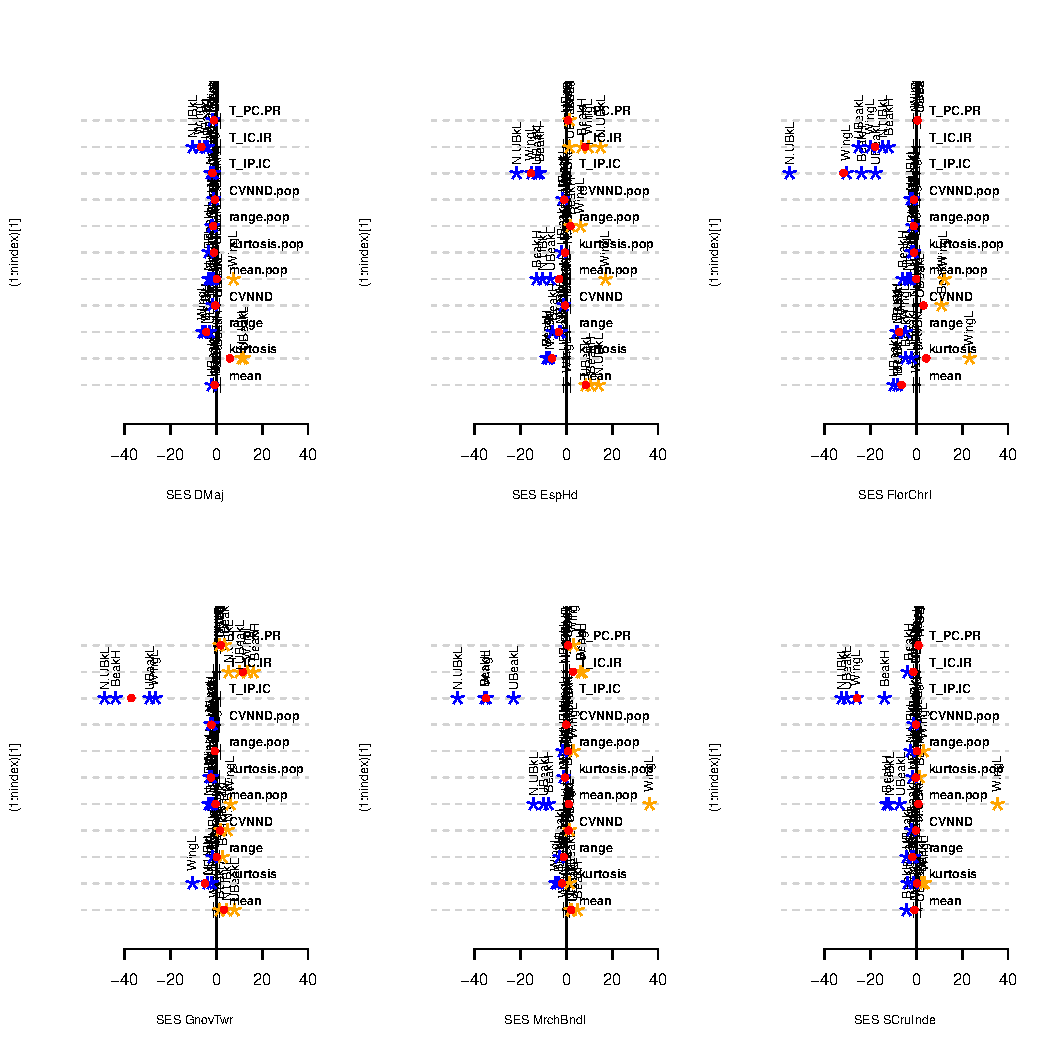
\includegraphics[width=\maxwidth]{figure/unnamed-chunk-421} 
\begin{kframe}\begin{alltt}
\hlkwd{par}\hlstd{(}\hlkwc{mfrow}\hlstd{=}\hlkwd{c}\hlstd{(}\hlnum{2}\hlstd{,}\hlnum{2}\hlstd{))}
\hlkwd{plot}\hlstd{(i.l1,}\hlkwc{type}\hlstd{=}\hlstr{"bytraits"}\hlstd{)}
\end{alltt}
\end{kframe}
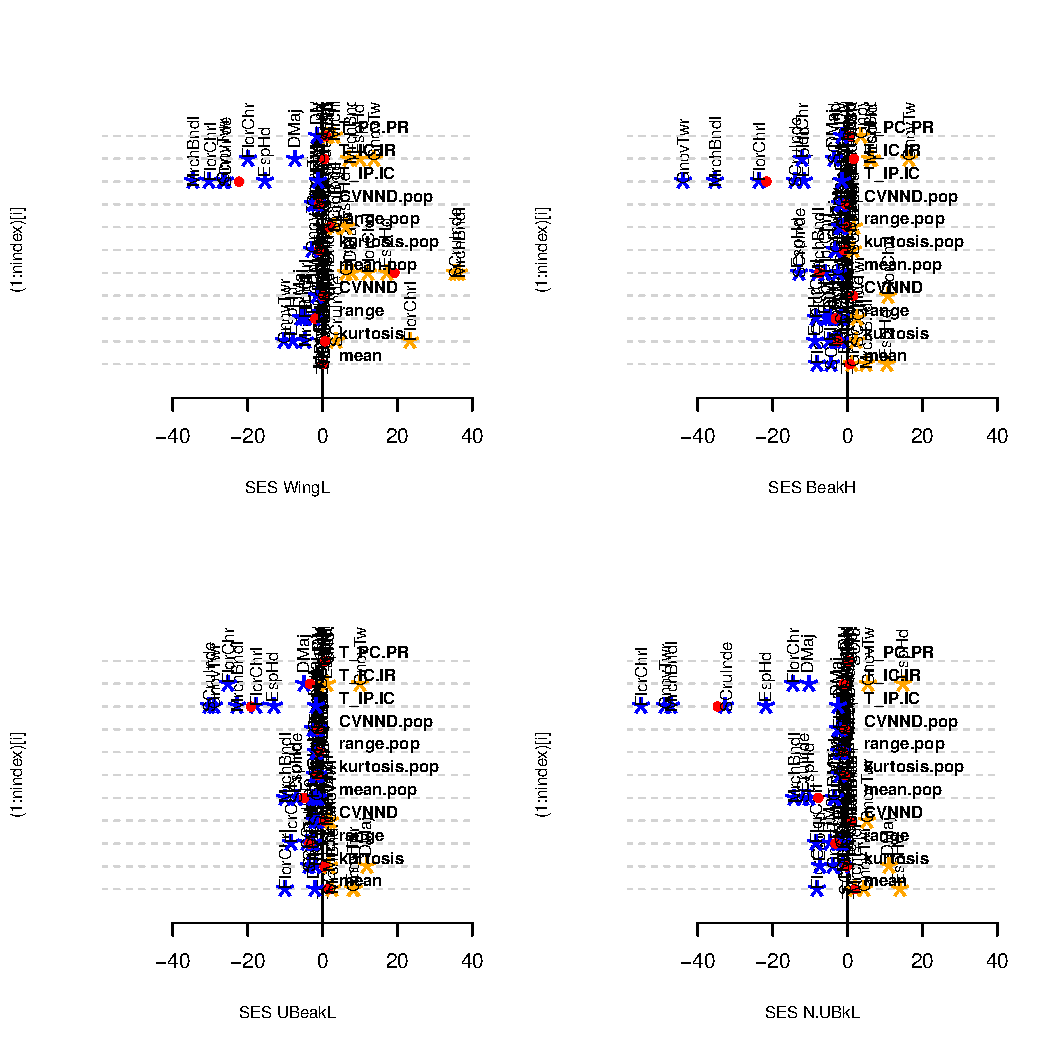
\includegraphics[width=\maxwidth]{figure/unnamed-chunk-422} 
\begin{kframe}\begin{alltt}
\hlkwd{par}\hlstd{(}\hlkwc{mfrow}\hlstd{=}\hlkwd{c}\hlstd{(}\hlnum{1}\hlstd{,}\hlnum{1}\hlstd{))}
\end{alltt}
\end{kframe}
\end{knitrout}

The other plot type are the same as plot.Tstats

\begin{knitrout}
\definecolor{shadecolor}{rgb}{0.969, 0.969, 0.969}\color{fgcolor}\begin{kframe}
\begin{alltt}
\hlkwd{par}\hlstd{(}\hlkwc{mfrow}\hlstd{=}\hlkwd{c}\hlstd{(}\hlnum{2}\hlstd{,}\hlnum{2}\hlstd{))}
\hlkwd{plot}\hlstd{(i.l1)}
\end{alltt}
\end{kframe}
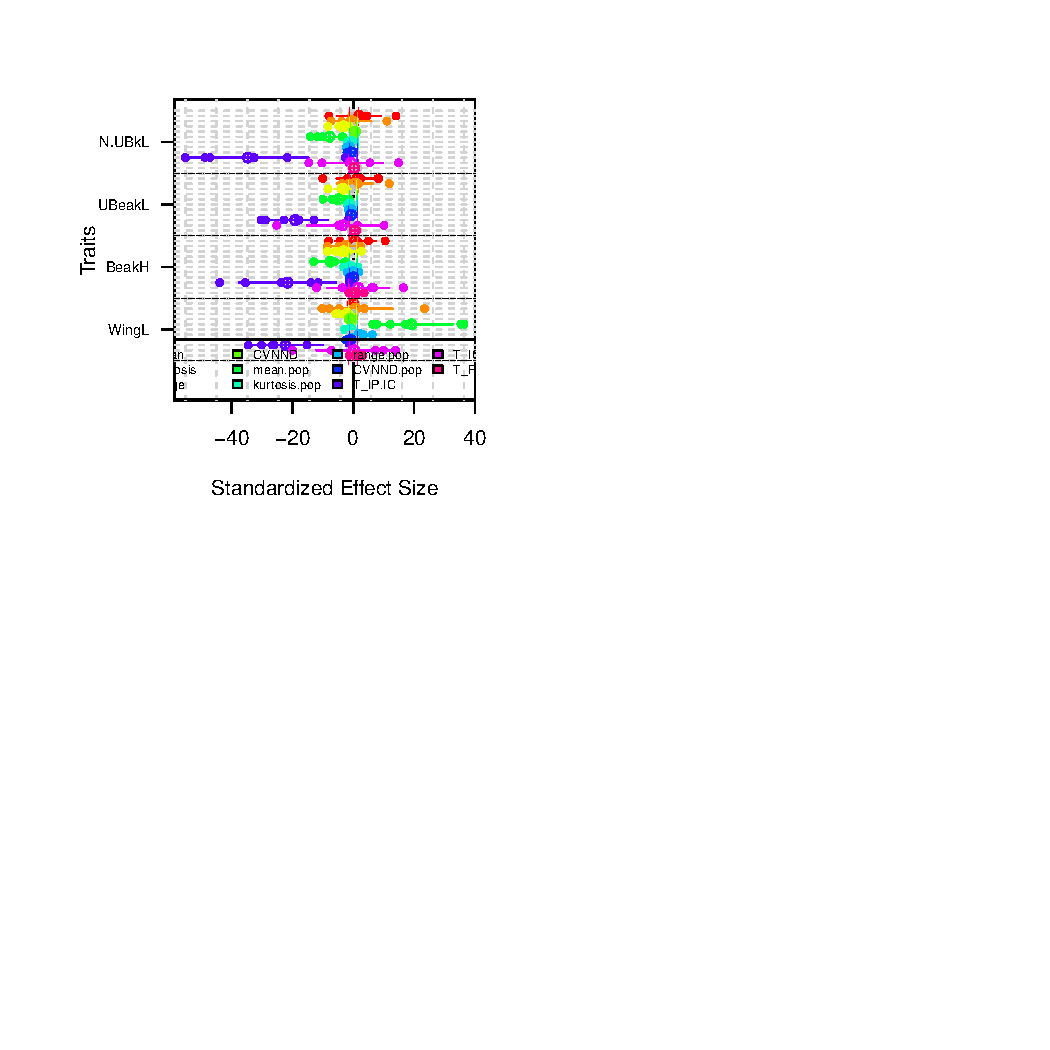
\includegraphics[width=\maxwidth]{figure/unnamed-chunk-431} 
\begin{kframe}\begin{alltt}
\hlkwd{plot}\hlstd{(i.l1,}\hlkwc{type}\hlstd{=}\hlstr{"simple_range"}\hlstd{)}
\end{alltt}
\end{kframe}
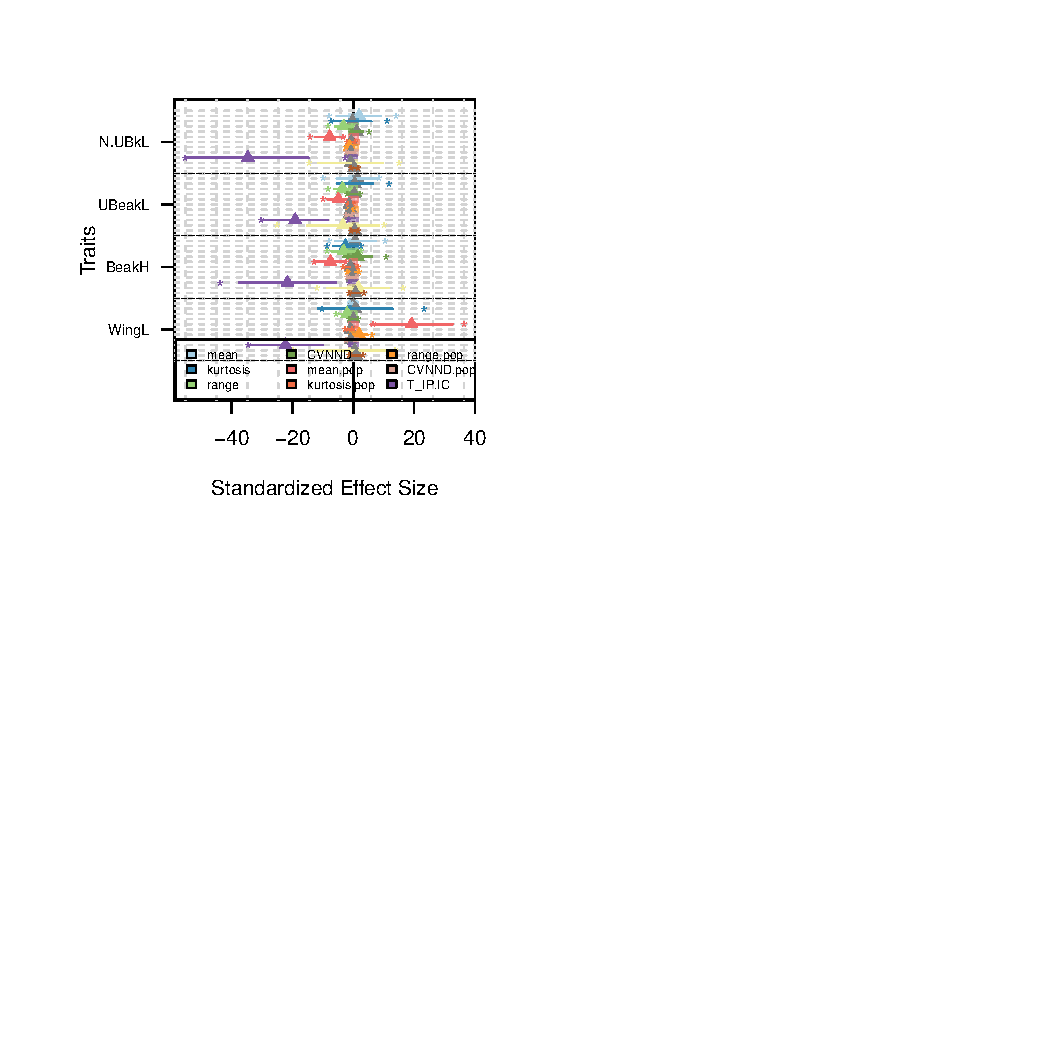
\includegraphics[width=\maxwidth]{figure/unnamed-chunk-432} 
\begin{kframe}\begin{alltt}
\hlkwd{plot}\hlstd{(i.l1,}\hlkwc{type}\hlstd{=}\hlstr{"normal"}\hlstd{)}
\end{alltt}
\end{kframe}
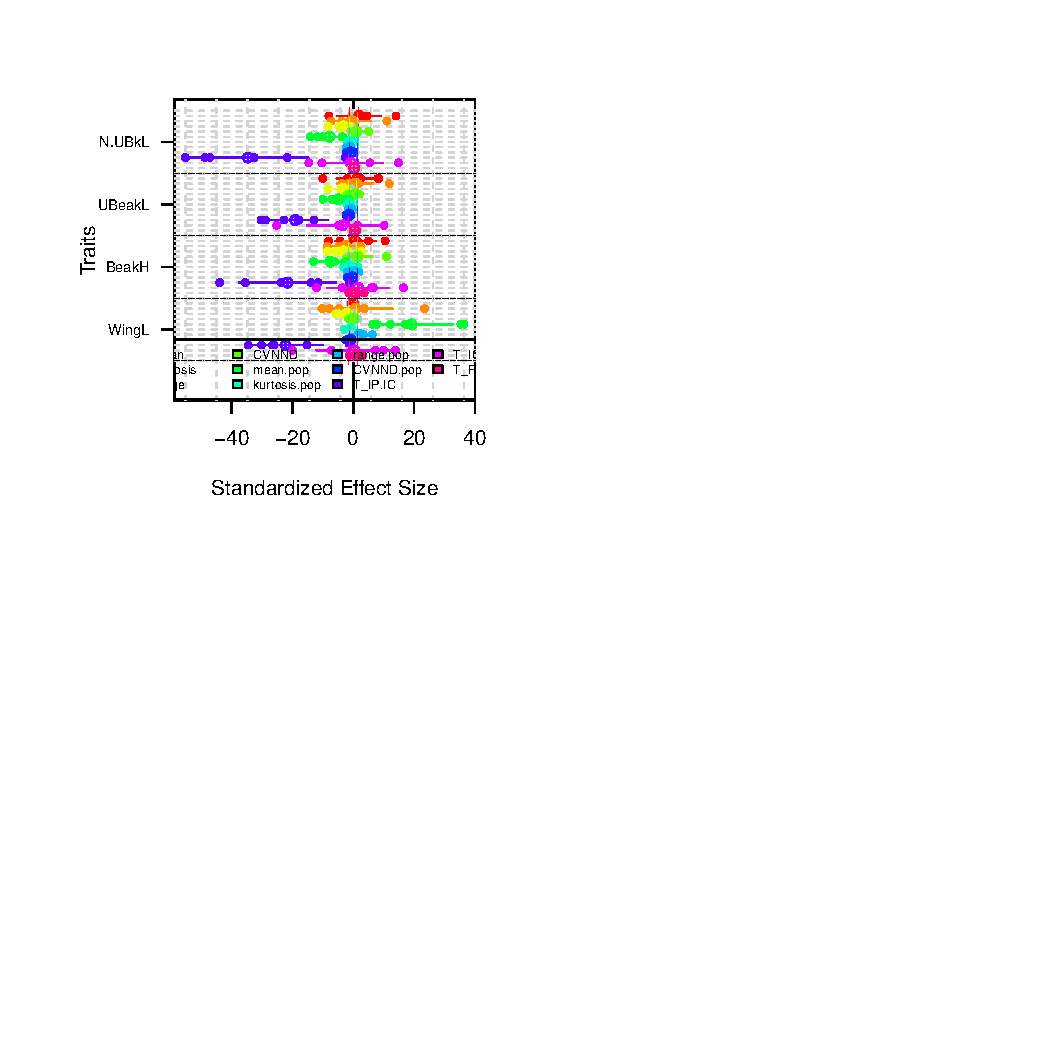
\includegraphics[width=\maxwidth]{figure/unnamed-chunk-433} 
\begin{kframe}\begin{alltt}
\hlkwd{plot}\hlstd{(i.l1,}\hlkwc{type}\hlstd{=}\hlstr{"barplot"}\hlstd{)}
\end{alltt}
\end{kframe}
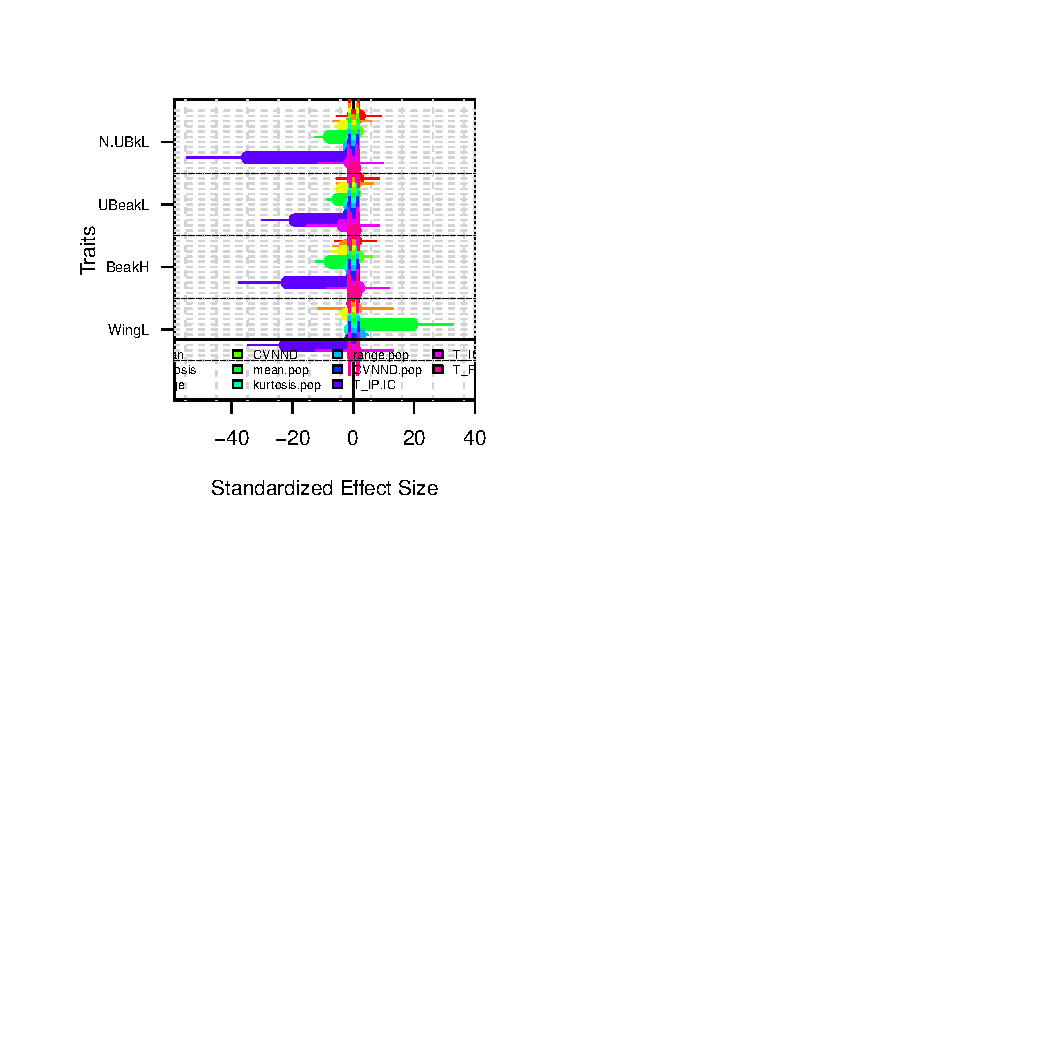
\includegraphics[width=\maxwidth]{figure/unnamed-chunk-434} 
\begin{kframe}\begin{alltt}
\hlkwd{par}\hlstd{(}\hlkwc{mfrow}\hlstd{=}\hlkwd{c}\hlstd{(}\hlnum{1}\hlstd{,}\hlnum{1}\hlstd{))}
\end{alltt}
\end{kframe}
\end{knitrout}



\newpage

\subsection{Multivariates index}

For most multivariate functions we need to replace (or exclude) NA values. For this example, we use the package mice to complete the data.

\begin{knitrout}
\definecolor{shadecolor}{rgb}{0.969, 0.969, 0.969}\color{fgcolor}\begin{kframe}
\begin{alltt}
\hlstd{comm}\hlkwb{<-}\hlkwd{t}\hlstd{(}\hlkwd{table}\hlstd{(ind.plot.finch,}\hlnum{1}\hlopt{:}\hlkwd{length}\hlstd{(ind.plot.finch)))}

\hlkwd{require}\hlstd{(mice)}
\hlstd{traits}\hlkwb{=}\hlstd{traits.finch}
\hlstd{mice}\hlkwb{<-}\hlkwd{mice}\hlstd{(traits.finch)}
\hlstd{traits.finch.mice}\hlkwb{<-}\hlkwd{complete}\hlstd{(mice)}
\end{alltt}
\end{kframe}
\end{knitrout}

A simple example to illustrate the concept of the function \tt{ComIndexMulti}

\begin{knitrout}
\definecolor{shadecolor}{rgb}{0.969, 0.969, 0.969}\color{fgcolor}\begin{kframe}
\begin{alltt}
\hlstd{n_sp_plot}\hlkwb{<-}\hlkwd{as.factor}\hlstd{(}\hlkwd{paste}\hlstd{(sp.finch, ind.plot.finch,} \hlkwc{sep}\hlstd{=}\hlstr{"_"}\hlstd{))}
\hlstd{res.sum.1}\hlkwb{<-}\hlkwd{ComIndexMulti}\hlstd{(traits.finch,}
                           \hlkwc{index}\hlstd{=}\hlkwd{c}\hlstd{(}\hlstr{"sum(scale(x), na.rm=T)"}\hlstd{,} \hlstr{"sum(x, na.rm=T)"}\hlstd{),}
                           \hlkwc{by.factor}\hlstd{=n_sp_plot,} \hlkwc{nullmodels}\hlstd{=}\hlkwd{c}\hlstd{(}\hlnum{2}\hlstd{,}\hlnum{2}\hlstd{),}
                           \hlkwc{ind.plot}\hlstd{=ind.plot.finch,} \hlkwc{nperm}\hlstd{=}\hlnum{9}\hlstd{,} \hlkwc{sp}\hlstd{=sp.finch)}
\end{alltt}
\begin{verbatim}
## [1] "creating null models"
## [1] "nm.2 25 %"
## [1] "nm.2 50 %"
## [1] "nm.2 75 %"
## [1] "nm.2 100 %"
## [1] "calculation of null values using null models"
## [1] "sum(scale(x), na.rm=T) 50 %"
## [1] "sum(x, na.rm=T) 100 %"
## [1] "calculation of observed values"
## [1] "50 %"
## [1] "100 %"
\end{verbatim}
\begin{alltt}
\hlkwd{attributes}\hlstd{(}\hlkwd{ses.listofindex}\hlstd{(}\hlkwd{as.listofindex}\hlstd{(}\hlkwd{list}\hlstd{(res.sum.1))))}
\end{alltt}
\begin{verbatim}
## $names
## [1] "index_1_1" "index_1_2"
## 
## $class
## [1] "ses.list"
\end{verbatim}
\end{kframe}
\end{knitrout}

\newpage
A more interesting example using the function \tt{hypervolume} from the package ... hypervolume.  We show here several results which differe in there factor that delimit the group to calculate different hypervolume (argument "byfactor"). 

First, let's try the hypervolume function one finch data.
\begin{knitrout}
\definecolor{shadecolor}{rgb}{0.969, 0.969, 0.969}\color{fgcolor}\begin{kframe}
\begin{alltt}
\hlstd{hv}\hlkwb{<-}\hlkwd{hypervolume}\hlstd{(traits.finch.mice,}
                \hlkwc{reps}\hlstd{=}\hlnum{100}\hlstd{,}\hlkwc{bandwidth}\hlstd{=}\hlnum{0.2}\hlstd{,}
                \hlkwc{verbose}\hlstd{=F,} \hlkwc{warnings}\hlstd{=F)}
\hlkwd{plot}\hlstd{(hv)}
\end{alltt}
\end{kframe}
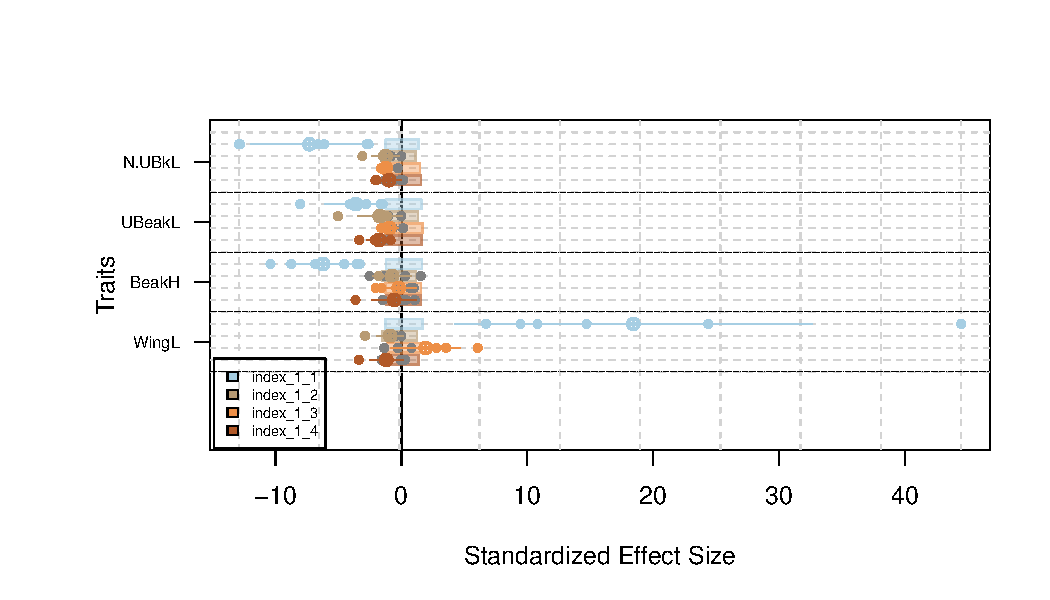
\includegraphics[width=\maxwidth]{figure/unnamed-chunk-46} 

\end{knitrout}

Now, we can do the same analysis for each species.

\begin{knitrout}
\definecolor{shadecolor}{rgb}{0.969, 0.969, 0.969}\color{fgcolor}\begin{kframe}
\begin{alltt}
\hlstd{hv.list}\hlkwb{<-}\hlkwd{new}\hlstd{(}\hlstr{"HypervolumeList"}\hlstd{)}
\hlstd{hv.list2}\hlkwb{<-}\hlkwd{list}\hlstd{()}

\hlkwa{for}\hlstd{(i} \hlkwa{in} \hlnum{1}\hlopt{:} \hlkwd{length}\hlstd{(}\hlkwd{table}\hlstd{(sp.finch))) \{}
  \hlstd{hv.list2[[i]]}\hlkwb{<-}\hlkwd{hypervolume}\hlstd{(traits.finch.mice[sp.finch}\hlopt{==}\hlkwd{levels}\hlstd{(sp.finch)[i], ],}
                \hlkwc{reps}\hlstd{=}\hlnum{1000}\hlstd{,}\hlkwc{bandwidth}\hlstd{=}\hlnum{0.2}\hlstd{,}
                \hlkwc{verbose}\hlstd{=F,} \hlkwc{warnings}\hlstd{=F)}
\hlstd{\}}

\hlstd{hv.list}\hlopt{@}\hlkwc{HVList}\hlkwb{<-}\hlstd{hv.list2}
\hlkwd{require}\hlstd{(adegenet)}
\end{alltt}


{\ttfamily\noindent\itshape\color{messagecolor}{\#\# Loading required package: adegenet\\\#\#\ \ \ \ ==========================\\\#\#\ \ \ \  adegenet 1.4-2 is loaded\\\#\#\ \ \ \ ==========================\\\#\# \\\#\#\ \ - to start, type '?adegenet'\\\#\#\ \ - to browse adegenet website, type 'adegenetWeb()'\\\#\#\ \ - to post questions/comments: adegenet-forum@lists.r-forge.r-project.org}}\begin{alltt}
\hlstd{colorhv}\hlkwb{<-}\hlkwd{transp}\hlstd{(}\hlkwd{funky}\hlstd{(}\hlkwd{nlevels}\hlstd{(sp.finch)),} \hlkwc{alpha}\hlstd{=}\hlnum{0.8}\hlstd{)}

\hlkwd{plot}\hlstd{(hv.list,} \hlkwc{colors}\hlstd{=colorhv,} \hlkwc{darkfactor}\hlstd{=}\hlnum{0.8}\hlstd{)}
\end{alltt}
\end{kframe}
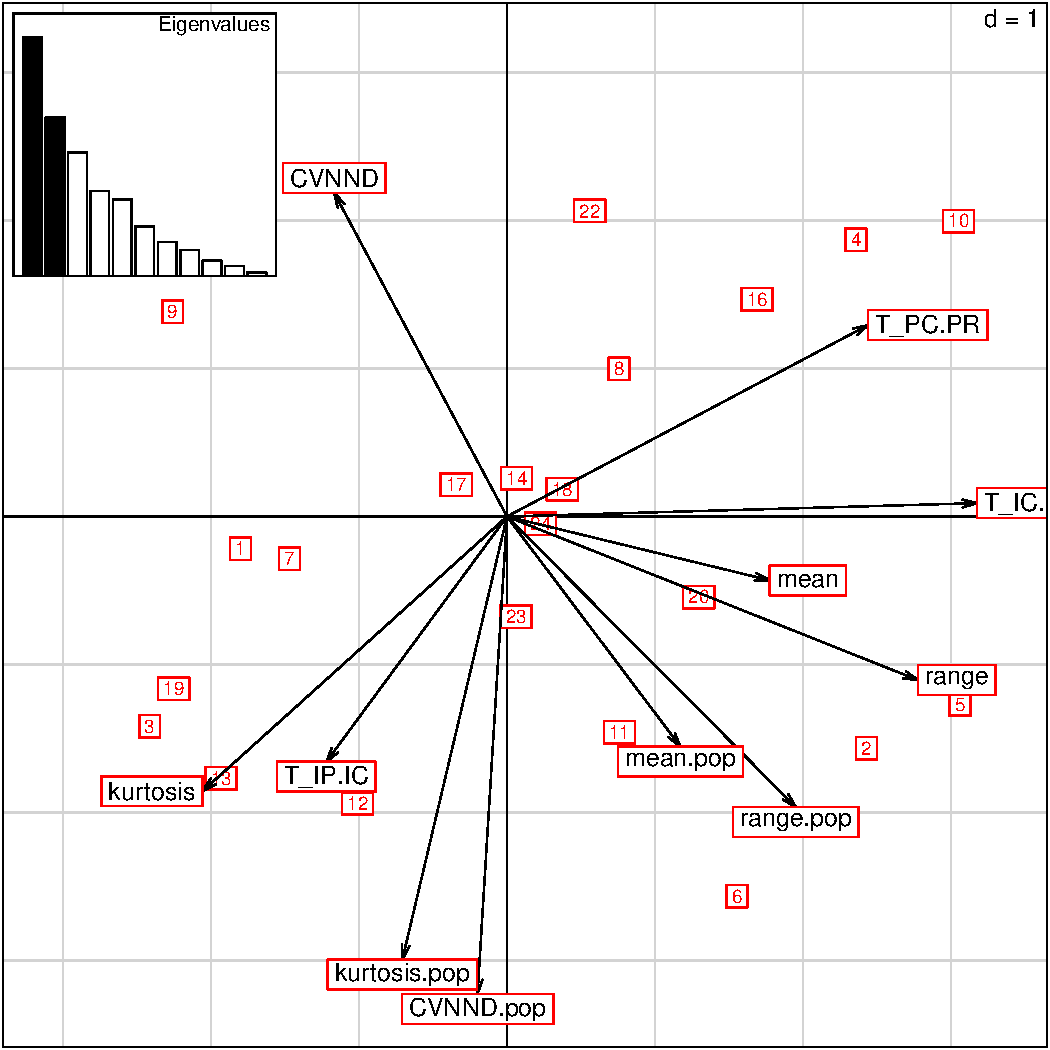
\includegraphics[width=\maxwidth]{figure/unnamed-chunk-471} 
\begin{kframe}\begin{alltt}
\hlkwd{plot}\hlstd{(hv.list,} \hlkwc{colors}\hlstd{=colorhv,} \hlkwc{darkfactor}\hlstd{=}\hlnum{0.8}\hlstd{,} \hlkwc{showdata}\hlstd{=F,} \hlkwc{npmax} \hlstd{=} \hlnum{200}\hlstd{,} \hlkwc{cex.random} \hlstd{=}\hlnum{1}\hlstd{)}
\end{alltt}
\end{kframe}
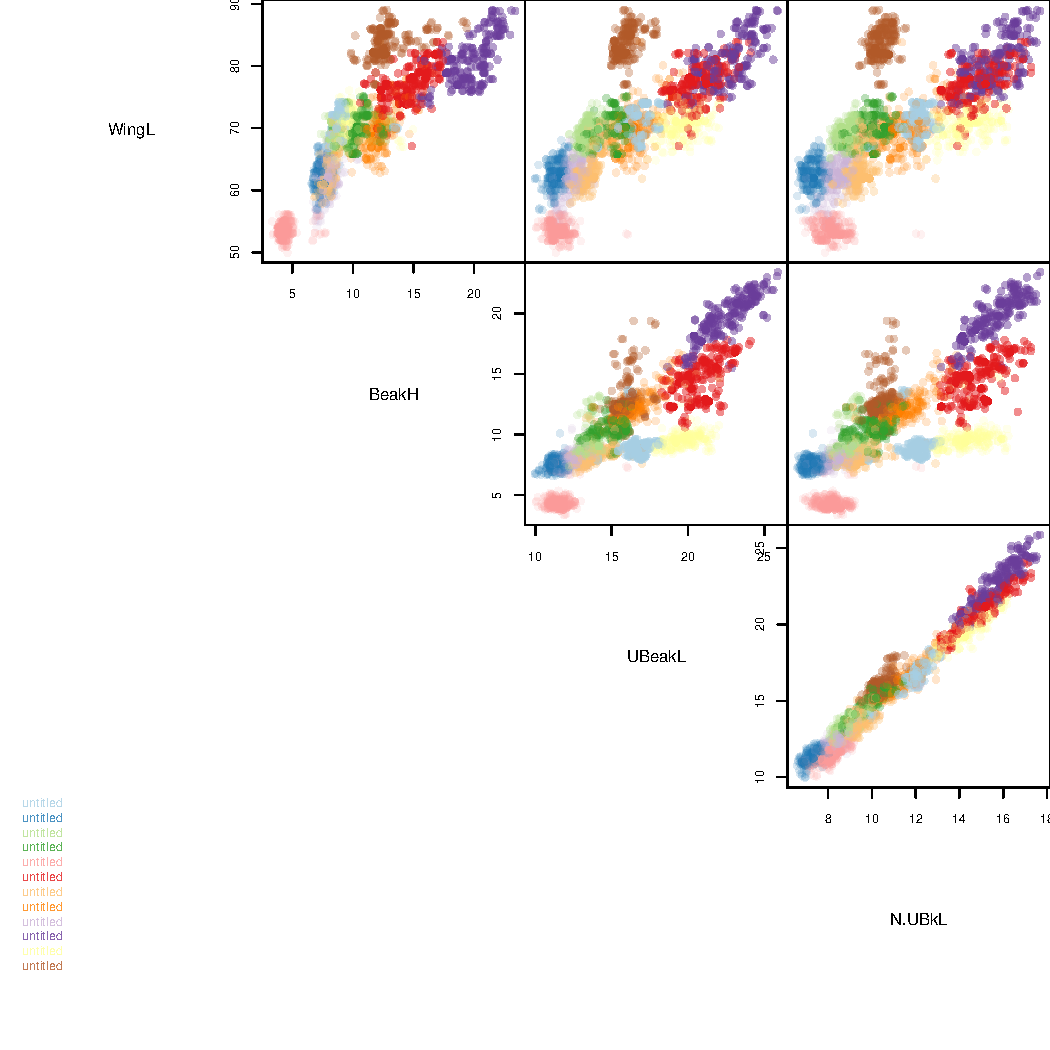
\includegraphics[width=\maxwidth]{figure/unnamed-chunk-472} 
\begin{kframe}\begin{alltt}
\hlkwd{summary}\hlstd{(hv.list)}
\end{alltt}
\begin{verbatim}
## HypervolumeList with 12 elements:
## 
## Hypervolume
## 	Name: untitled
## 	Nr. of observations: 23
## 	Dimensionality: 4
## 	Volume: 0.581274
## 	Bandwidth: 0.2 0.2 0.2 0.2
## 	Disjunct factor: 0.987217
## 	Quantile desired: 0.000000
## 	Quantile obtained: 0.000000
## 	Nr. of repetitions per point: 1000
## 	Number of random points: 14385
## Hypervolume
## 	Name: untitled
## 	Nr. of observations: 172
## 	Dimensionality: 4
## 	Volume: 3.508501
## 	Bandwidth: 0.2 0.2 0.2 0.2
## 	Disjunct factor: 0.796807
## 	Quantile desired: 0.000000
## 	Quantile obtained: 0.000000
## 	Nr. of repetitions per point: 1000
## 	Number of random points: 91104
## Hypervolume
## 	Name: untitled
## 	Nr. of observations: 142
## 	Dimensionality: 4
## 	Volume: 2.957552
## 	Bandwidth: 0.2 0.2 0.2 0.2
## 	Disjunct factor: 0.813587
## 	Quantile desired: 0.000000
## 	Quantile obtained: 0.000000
## 	Nr. of repetitions per point: 1000
## 	Number of random points: 76385
## Hypervolume
## 	Name: untitled
## 	Nr. of observations: 73
## 	Dimensionality: 4
## 	Volume: 1.729685
## 	Bandwidth: 0.2 0.2 0.2 0.2
## 	Disjunct factor: 0.925559
## 	Quantile desired: 0.000000
## 	Quantile obtained: 0.000000
## 	Nr. of repetitions per point: 1000
## 	Number of random points: 43564
## Hypervolume
## 	Name: untitled
## 	Nr. of observations: 299
## 	Dimensionality: 4
## 	Volume: 4.127026
## 	Bandwidth: 0.2 0.2 0.2 0.2
## 	Disjunct factor: 0.539170
## 	Quantile desired: 0.000000
## 	Quantile obtained: 0.000000
## 	Nr. of repetitions per point: 1000
## 	Number of random points: 114079
## Hypervolume
## 	Name: untitled
## 	Nr. of observations: 206
## 	Dimensionality: 4
## 	Volume: 5.070588
## 	Bandwidth: 0.2 0.2 0.2 0.2
## 	Disjunct factor: 0.961504
## 	Quantile desired: 0.000000
## 	Quantile obtained: 0.000000
## 	Nr. of repetitions per point: 1000
## 	Number of random points: 126546
## Hypervolume
## 	Name: untitled
## 	Nr. of observations: 125
## 	Dimensionality: 4
## 	Volume: 2.734825
## 	Bandwidth: 0.2 0.2 0.2 0.2
## 	Disjunct factor: 0.854633
## 	Quantile desired: 0.000000
## 	Quantile obtained: 0.000000
## 	Nr. of repetitions per point: 1000
## 	Number of random points: 69799
## Hypervolume
## 	Name: untitled
## 	Nr. of observations: 548
## 	Dimensionality: 4
## 	Volume: 11.785994
## 	Bandwidth: 0.2 0.2 0.2 0.2
## 	Disjunct factor: 0.840128
## 	Quantile desired: 0.000000
## 	Quantile obtained: 0.000000
## 	Nr. of repetitions per point: 1000
## 	Number of random points: 302349
## Hypervolume
## 	Name: untitled
## 	Nr. of observations: 386
## 	Dimensionality: 4
## 	Volume: 6.293490
## 	Bandwidth: 0.2 0.2 0.2 0.2
## 	Disjunct factor: 0.636890
## 	Quantile desired: 0.000000
## 	Quantile obtained: 0.000000
## 	Nr. of repetitions per point: 1000
## 	Number of random points: 170580
## Hypervolume
## 	Name: untitled
## 	Nr. of observations: 126
## 	Dimensionality: 4
## 	Volume: 3.180147
## 	Bandwidth: 0.2 0.2 0.2 0.2
## 	Disjunct factor: 0.985909
## 	Quantile desired: 0.000000
## 	Quantile obtained: 0.000000
## 	Nr. of repetitions per point: 1000
## 	Number of random points: 78794
## Hypervolume
## 	Name: untitled
## 	Nr. of observations: 284
## 	Dimensionality: 4
## 	Volume: 6.331289
## 	Bandwidth: 0.2 0.2 0.2 0.2
## 	Disjunct factor: 0.870831
## 	Quantile desired: 0.000000
## 	Quantile obtained: 0.000000
## 	Nr. of repetitions per point: 1000
## 	Number of random points: 161250
## Hypervolume
## 	Name: untitled
## 	Nr. of observations: 129
## 	Dimensionality: 4
## 	Volume: 2.871520
## 	Bandwidth: 0.2 0.2 0.2 0.2
## 	Disjunct factor: 0.869525
## 	Quantile desired: 0.000000
## 	Quantile obtained: 0.000000
## 	Nr. of repetitions per point: 1000
## 	Number of random points: 72987
\end{verbatim}
\end{kframe}
\end{knitrout}

The standard example of the hypervolume package also use finch data but at the species level.

\begin{knitrout}
\definecolor{shadecolor}{rgb}{0.969, 0.969, 0.969}\color{fgcolor}\begin{kframe}
\begin{alltt}
\hlkwd{demo}\hlstd{(}\hlstr{'finch'}\hlstd{,} \hlkwc{package}\hlstd{=}\hlstr{'hypervolume'}\hlstd{)}
\end{alltt}
\begin{verbatim}
## 
## 
## 	demo(finch)
## 	---- ~~~~~
## 
## > if (exists('doHypervolumeFinchDemo')==TRUE)
## + {
## +   data(finch)
## +   
## +   species_list = unique(finch$Species)
## +   num_species = length(species_list)
## +   
## +   hv_finches_list = new("HypervolumeList")
## +   hv_finches_list@HVList = vector(mode="list",length=num_species)
## +   
## +   # compute hypervolumes for each species
## +   for (i in 1:num_species)
## +   {
## +     this_species = subset(finch, Species==species_list[i])
## +     # keep the trait data
## +     this_species_log <- log10(this_species[,2:ncol(this_species)])
## +     # make a hypervolume using auto-bandwidth
## +     hv_finches_list@HVList[[i]] <- hypervolume(this_species_log, bandwidth=estimate_bandwidth(this_species_log),
## +                                                reps=10000, quantile=0, name=as.character(species_list[i]), warn=FALSE)
## +   }
## +   
## +   # compute all pairwise overlaps
## +   overlap = matrix(NA, nrow=num_species, ncol=num_species)
## +   dimnames(overlap)=list(species_list, species_list)
## +   for (i in 1:num_species)
## +   {
## +     for (j in i:num_species)
## +     {
## +       if (i!=j)
## +       {
## +         # compute set operations on each pair
## +         this_set = hypervolume_set(hv_finches_list@HVList[[i]], hv_finches_list@HVList[[j]],reduction_factor=0.5, check_memory=FALSE)
## +         # calculate a Sorensen overlap index (2 x shared volume / sum of |hv1| + |hv2|)
## +         overlap[i,j] = 2 * this_set@HVList$Intersection@Volume / (hv_finches_list@HVList[[i]]@Volume + hv_finches_list@HVList[[j]]@Volume)
## +       }
## +     }   
## +   }
## +   
## + 
## +   
## +   # show all hypervolumes
## +   plot(hv_finches_list,npmax=500,darkfactor=0.5,cex.legend=0.25,cex.names=0.75)
## +   
## +   # show pairwise overlaps - note that actually very few species overlap in nine dimensions
## +   op <- par(mar=c(10,10,1,1))
## +   image(x=1:nrow(overlap), y=1:nrow(overlap), z=overlap,axes=F,xlab='',ylab='',col=rainbow(5))
## +   box()
## +   axis(side=1, at=1:(length(dimnames(overlap)[[1]])),dimnames(overlap)[[1]],las=2,cex.axis=0.75)
## +   axis(side=2, at=1:(length(dimnames(overlap)[[2]])),dimnames(overlap)[[2]],las=1,cex.axis=0.75)
## +   par(op)
## +   
## +   rm(doHypervolumeFinchDemo)
## + } else
## + {
## +   message('Demo does not run by default to meet CRAN runtime requirements.')
## +   message('This demo requires approximately 3 minutes to run.')  
## +   message('To run the demo, type')
## +   message('\tdoHypervolumeFinchDemo=TRUE')
## +   message('\tdemo(finch)')
## +   message('at the R command line prompt.')
## + }
\end{verbatim}


{\ttfamily\noindent\itshape\color{messagecolor}{\#\# Demo does not run by default to meet CRAN runtime requirements.\\\#\# This demo requires approximately 3 minutes to run.\\\#\# To run the demo, type\\\#\# 	doHypervolumeFinchDemo=TRUE\\\#\# 	demo(finch)\\\#\# at the R command line prompt.}}\end{kframe}
\end{knitrout}

\tt{ComIndexMulti} takes the same arguments as \tt{ComIndex} and an argument by factor to apply the index on different factors.

\begin{knitrout}
\definecolor{shadecolor}{rgb}{0.969, 0.969, 0.969}\color{fgcolor}\begin{kframe}
\begin{alltt}
\hlcom{#all individual are put in the same group: calcul the hypervolume without by.factor}
\hlstd{hv.1}\hlkwb{<-}\hlkwd{ComIndexMulti}\hlstd{(traits.finch.mice,}
                          \hlkwc{index}\hlstd{=}\hlkwd{c}\hlstd{(}\hlstr{"as.numeric(try(hypervolume(na.omit(x), reps=100, 
                                  bandwidth=0.2, verbose=F, warnings=F)@Volume))"}\hlstd{),}
                          \hlkwc{by.factor}\hlstd{=}\hlkwd{rep}\hlstd{(}\hlnum{1}\hlstd{,}\hlkwd{length}\hlstd{(n_sp_plot)),} \hlkwc{nullmodels}\hlstd{=}\hlkwd{c}\hlstd{(}\hlnum{2}\hlstd{,}\hlnum{2}\hlstd{),}
                          \hlkwc{ind.plot}\hlstd{=ind.plot.finch,} \hlkwc{nperm}\hlstd{=}\hlnum{9}\hlstd{,} \hlkwc{sp}\hlstd{=sp.finch)}
\end{alltt}
\begin{verbatim}
## [1] "creating null models"
## [1] "nm.2 25 %"
## [1] "nm.2 50 %"
## [1] "nm.2 75 %"
## [1] "nm.2 100 %"
## [1] "calculation of null values using null models"
## [1] "as.numeric(try(hypervolume(na.omit(x), reps=100, \n                                  bandwidth=0.2, verbose=F, warnings=F)@Volume)) 100 %"
## [1] "calculation of observed values"
## [1] "100 %"
\end{verbatim}
\begin{alltt}
\hlstd{hv.2}\hlkwb{<-}\hlkwd{ComIndexMulti}\hlstd{(traits.finch.mice,}
                          \hlkwc{index}\hlstd{=}\hlkwd{c}\hlstd{(}\hlstr{"as.numeric(try(hypervolume(na.omit(x), reps=100, 
                                  bandwidth=0.2, verbose=F, warnings=F)@Volume))"}\hlstd{),}
                          \hlkwc{by.factor}\hlstd{=n_sp_plot,} \hlkwc{nullmodels}\hlstd{=}\hlkwd{c}\hlstd{(}\hlnum{2}\hlstd{,}\hlnum{2}\hlstd{),}
                          \hlkwc{ind.plot}\hlstd{=ind.plot.finch,} \hlkwc{nperm}\hlstd{=}\hlnum{9}\hlstd{,} \hlkwc{sp}\hlstd{=sp.finch)}
\end{alltt}
\begin{verbatim}
## [1] "creating null models"
## [1] "nm.2 25 %"
## [1] "nm.2 50 %"
## [1] "nm.2 75 %"
## [1] "nm.2 100 %"
## [1] "calculation of null values using null models"
## [1] "as.numeric(try(hypervolume(na.omit(x), reps=100, \n                                  bandwidth=0.2, verbose=F, warnings=F)@Volume)) 100 %"
## [1] "calculation of observed values"
## [1] "100 %"
\end{verbatim}
\begin{alltt}
\hlstd{hv.3}\hlkwb{<-}\hlkwd{ComIndexMulti}\hlstd{(traits.finch.mice,}
                          \hlkwc{index}\hlstd{=}\hlkwd{c}\hlstd{(}\hlstr{"as.numeric(try(hypervolume(na.omit(x), reps=100,
                                  bandwidth=0.2, verbose=F, warnings=F)@Volume))"}\hlstd{),}
                          \hlkwc{by.factor}\hlstd{=ind.plot.finch,} \hlkwc{nullmodels}\hlstd{=}\hlkwd{c}\hlstd{(}\hlnum{2}\hlstd{,}\hlnum{2}\hlstd{),}
                          \hlkwc{ind.plot}\hlstd{=ind.plot.finch,} \hlkwc{nperm}\hlstd{=}\hlnum{9}\hlstd{,} \hlkwc{sp}\hlstd{=sp.finch)}
\end{alltt}
\begin{verbatim}
## [1] "creating null models"
## [1] "nm.2 25 %"
## [1] "nm.2 50 %"
## [1] "nm.2 75 %"
## [1] "nm.2 100 %"
## [1] "calculation of null values using null models"
## [1] "as.numeric(try(hypervolume(na.omit(x), reps=100,\n                                  bandwidth=0.2, verbose=F, warnings=F)@Volume)) 100 %"
## [1] "calculation of observed values"
## [1] "100 %"
\end{verbatim}
\begin{alltt}
\hlstd{hv.4}\hlkwb{<-}\hlkwd{ComIndexMulti}\hlstd{(traits.finch.mice,}
                          \hlkwc{index}\hlstd{=}\hlkwd{c}\hlstd{(}\hlstr{"as.numeric(try(hypervolume(na.omit(x), reps=100, 
                                  bandwidth=0.2, verbose=F, warnings=F)@Volume))"}\hlstd{),}
                          \hlkwc{by.factor}\hlstd{=sp.finch,} \hlkwc{nullmodels}\hlstd{=}\hlkwd{c}\hlstd{(}\hlnum{2}\hlstd{,}\hlnum{2}\hlstd{),}
                          \hlkwc{ind.plot}\hlstd{=ind.plot.finch,} \hlkwc{nperm}\hlstd{=}\hlnum{9}\hlstd{,} \hlkwc{sp}\hlstd{=sp.finch)}
\end{alltt}
\begin{verbatim}
## [1] "creating null models"
## [1] "nm.2 25 %"
## [1] "nm.2 50 %"
## [1] "nm.2 75 %"
## [1] "nm.2 100 %"
## [1] "calculation of null values using null models"
## [1] "as.numeric(try(hypervolume(na.omit(x), reps=100, \n                                  bandwidth=0.2, verbose=F, warnings=F)@Volume)) 100 %"
## [1] "calculation of observed values"
## [1] "100 %"
\end{verbatim}
\begin{alltt}
\hlstd{list.ind.multi}\hlkwb{<-}\hlkwd{as.listofindex}\hlstd{(}\hlkwd{list}\hlstd{(hv.2, hv.3, hv.4))}

\hlstd{ses.list.multi}\hlkwb{<-}\hlkwd{ses.listofindex}\hlstd{(list.ind.multi)}
\end{alltt}
\end{kframe}
\end{knitrout}

\begin{knitrout}
\definecolor{shadecolor}{rgb}{0.969, 0.969, 0.969}\color{fgcolor}\begin{kframe}
\begin{alltt}
\hlkwd{plot}\hlstd{(list.ind.multi)}
\end{alltt}
\end{kframe}
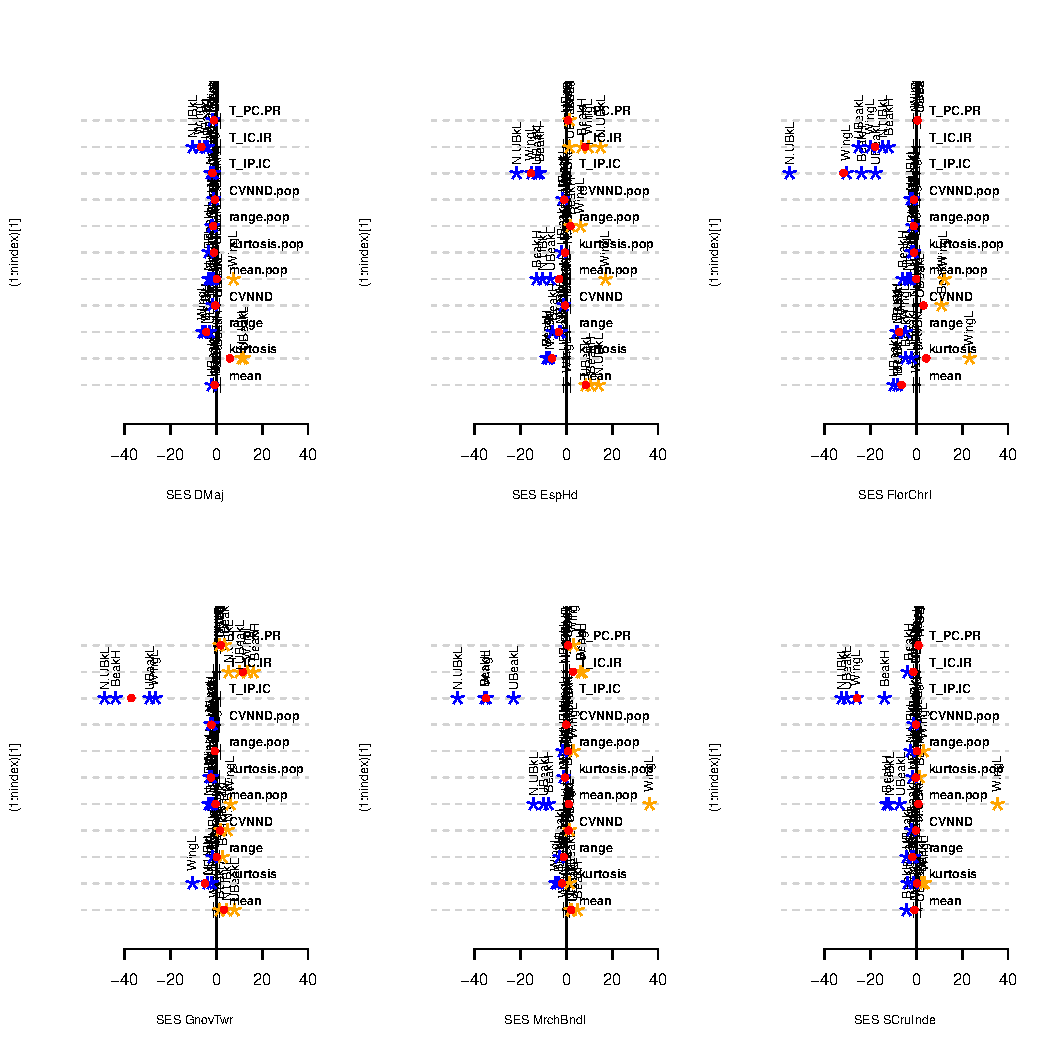
\includegraphics[width=\maxwidth]{figure/unnamed-chunk-501} 
\begin{kframe}\begin{alltt}
\hlkwd{plot}\hlstd{(list.ind.multi,} \hlkwc{xlim}\hlstd{=}\hlkwd{c}\hlstd{(}\hlopt{-}\hlnum{200}\hlstd{,}\hlnum{20}\hlstd{))}
\end{alltt}
\end{kframe}
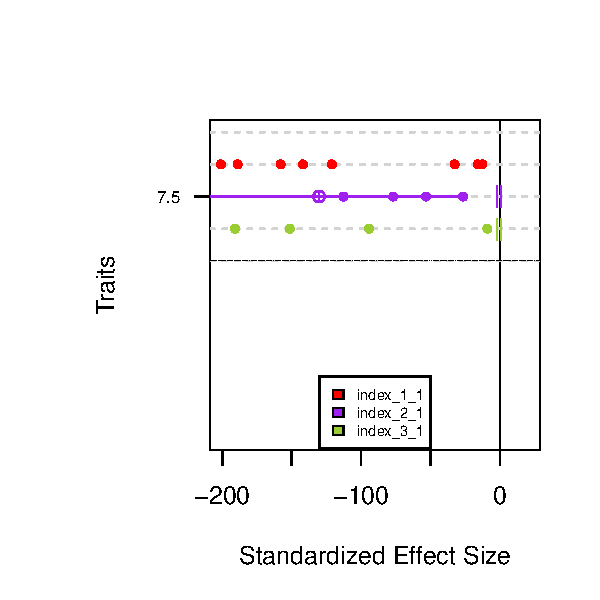
\includegraphics[width=\maxwidth]{figure/unnamed-chunk-502} 

\end{knitrout}

Compare hypervolume to Villéger metrics convex hull.

\begin{knitrout}
\definecolor{shadecolor}{rgb}{0.969, 0.969, 0.969}\color{fgcolor}\begin{kframe}
\begin{alltt}
\hlkwd{require}\hlstd{(}\hlstr{"geometry"}\hlstd{)}
\end{alltt}


{\ttfamily\noindent\itshape\color{messagecolor}{\#\# Loading required package: geometry\\\#\# Loading required package: magic\\\#\# Loading required package: abind}}\begin{alltt}
\hlstd{FA}\hlkwb{<-}\hlkwd{as.character}\hlstd{(}\hlstr{"FA"}\hlstd{)}
\hlstd{funct}\hlkwb{<-}\hlkwd{c}\hlstd{(}\hlstr{"round(convhulln(x,FA)$vol,6)"}\hlstd{)}

\hlcom{##Null model 1 is trivial for this function}
\hlcom{##because randomisation is within community only}
\hlstd{Fdis.finch}\hlkwb{<-}\hlkwd{ComIndexMulti}\hlstd{(traits.finch.mice,}
                          \hlkwc{index}\hlstd{=funct,}
                          \hlkwc{by.factor}\hlstd{=ind.plot.finch,} \hlkwc{nullmodels}\hlstd{=}\hlkwd{c}\hlstd{(}\hlnum{2}\hlstd{,}\hlnum{2}\hlstd{),}
                          \hlkwc{ind.plot}\hlstd{=ind.plot.finch,} \hlkwc{nperm}\hlstd{=}\hlnum{9}\hlstd{,} \hlkwc{sp}\hlstd{=sp.finch)}
\end{alltt}
\begin{verbatim}
## [1] "creating null models"
## [1] "nm.2 25 %"
## [1] "nm.2 50 %"
## [1] "nm.2 75 %"
## [1] "nm.2 100 %"
## [1] "calculation of null values using null models"
## [1] "round(convhulln(x,FA)$vol,6) 100 %"
## [1] "calculation of observed values"
## [1] "100 %"
\end{verbatim}
\begin{alltt}
\hlstd{list.ind.multi2}\hlkwb{<-}\hlkwd{as.listofindex}\hlstd{(}\hlkwd{list}\hlstd{(hv.3, Fdis.finch))}

\hlstd{ses.list.multi2}\hlkwb{<-}\hlkwd{ses.listofindex}\hlstd{(list.ind.multi2)}
\end{alltt}
\end{kframe}
\end{knitrout}

\begin{knitrout}
\definecolor{shadecolor}{rgb}{0.969, 0.969, 0.969}\color{fgcolor}\begin{kframe}
\begin{alltt}
\hlkwd{plot}\hlstd{(list.ind.multi2)}
\end{alltt}
\end{kframe}
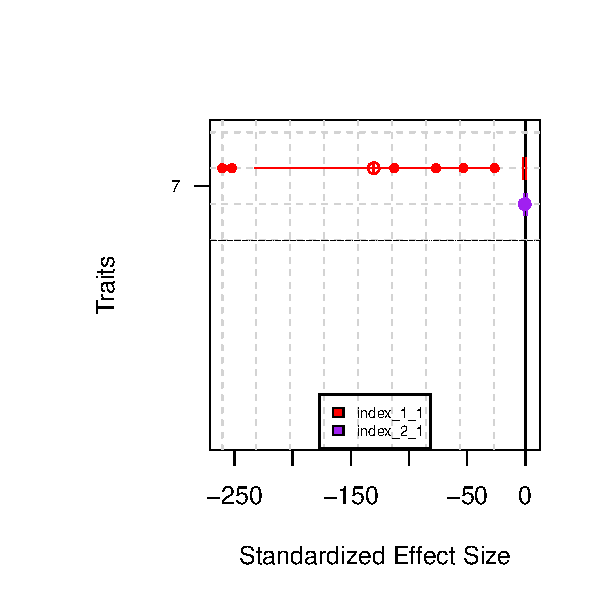
\includegraphics[width=\maxwidth]{figure/unnamed-chunk-52} 

\end{knitrout}

\section{Others graphics functions}

Using rasterVis to obtain more color schemes. 
\begin{knitrout}
\definecolor{shadecolor}{rgb}{0.969, 0.969, 0.969}\color{fgcolor}\begin{kframe}


{\ttfamily\noindent\itshape\color{messagecolor}{\#\# Loading required package: rasterVis\\\#\# Loading required package: raster\\\#\# Loading required package: sp\\\#\# \\\#\# Attaching package: 'raster'\\\#\# \\\#\# The following object is masked from 'package:magic':\\\#\# \\\#\#\ \ \ \  shift\\\#\# \\\#\# The following objects are masked from 'package:ape':\\\#\# \\\#\#\ \ \ \  edges, rotate, zoom\\\#\# \\\#\# The following object is masked from 'package:nlme':\\\#\# \\\#\#\ \ \ \  getData\\\#\# \\\#\# Loading required package: latticeExtra\\\#\# Loading required package: RColorBrewer\\\#\# Loading required package: hexbin}}\end{kframe}
\end{knitrout}

Plot the p-value or the ses values using the function \tt{levelplot}.

\begin{knitrout}
\definecolor{shadecolor}{rgb}{0.969, 0.969, 0.969}\color{fgcolor}\begin{kframe}
\begin{alltt}
\hlkwd{levelplot}\hlstd{(}\hlkwd{t}\hlstd{(}\hlkwd{sum_Tstats}\hlstd{(res.finch)}\hlopt{$}\hlstd{p.value),}
          \hlkwc{colorkey}\hlstd{=my.ckey,} \hlkwc{par.settings}\hlstd{=my.theme,}\hlkwc{border}\hlstd{=}\hlstr{"black"}\hlstd{)}
\end{alltt}
\end{kframe}
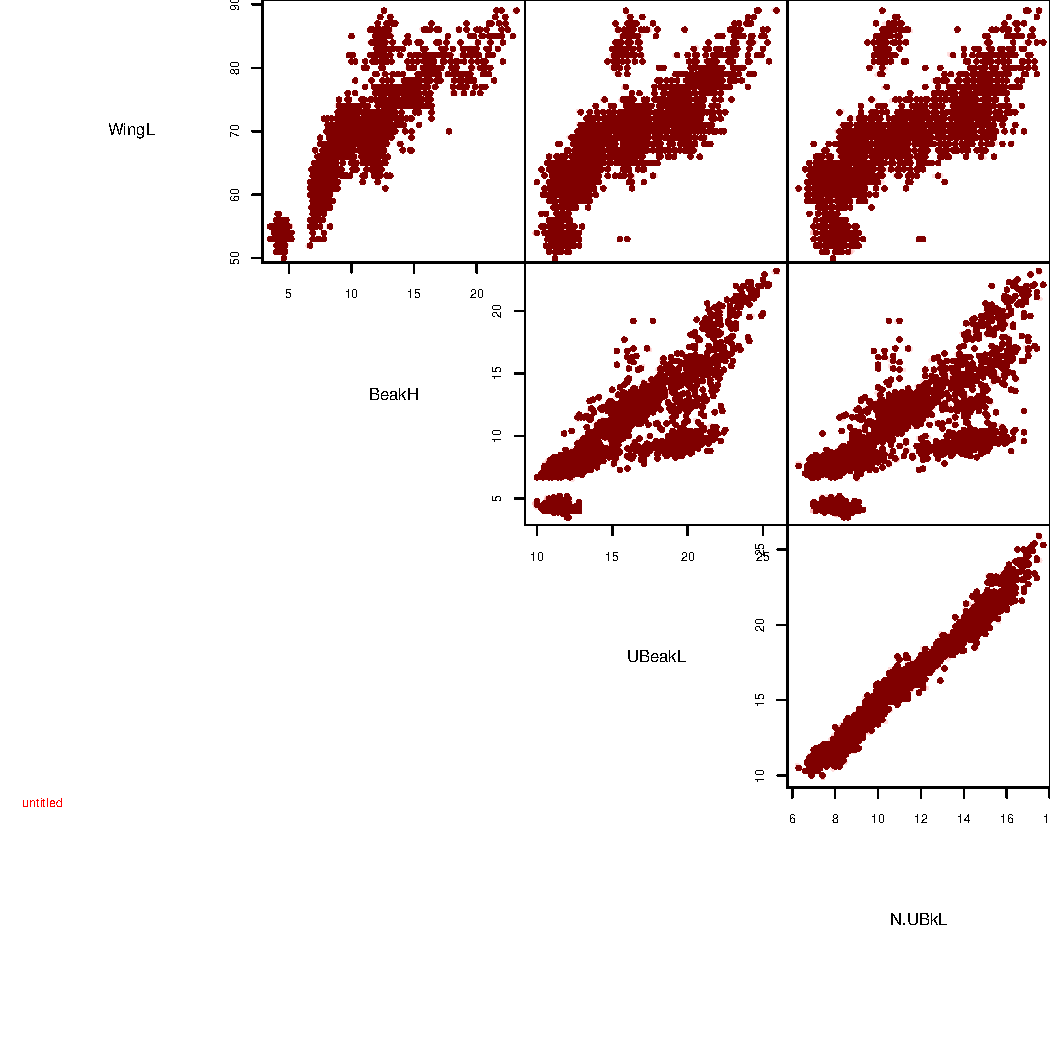
\includegraphics[width=\maxwidth]{figure/unnamed-chunk-54} 

\end{knitrout}


\begin{knitrout}
\definecolor{shadecolor}{rgb}{0.969, 0.969, 0.969}\color{fgcolor}\begin{kframe}
\begin{alltt}
\hlkwd{levelplot}\hlstd{(}\hlkwd{t}\hlstd{(}\hlkwd{ses}\hlstd{(res.finch}\hlopt{$}\hlstd{Tstats}\hlopt{$}\hlstd{T_IP.IC, res.finch}\hlopt{$}\hlstd{Tstats}\hlopt{$}\hlstd{T_IP.IC_nm)}\hlopt{$}\hlstd{ses),}
          \hlkwc{colorkey}\hlstd{=my.ckey,} \hlkwc{par.settings}\hlstd{=my.theme,}\hlkwc{border}\hlstd{=}\hlstr{"black"}\hlstd{)}
\end{alltt}
\end{kframe}
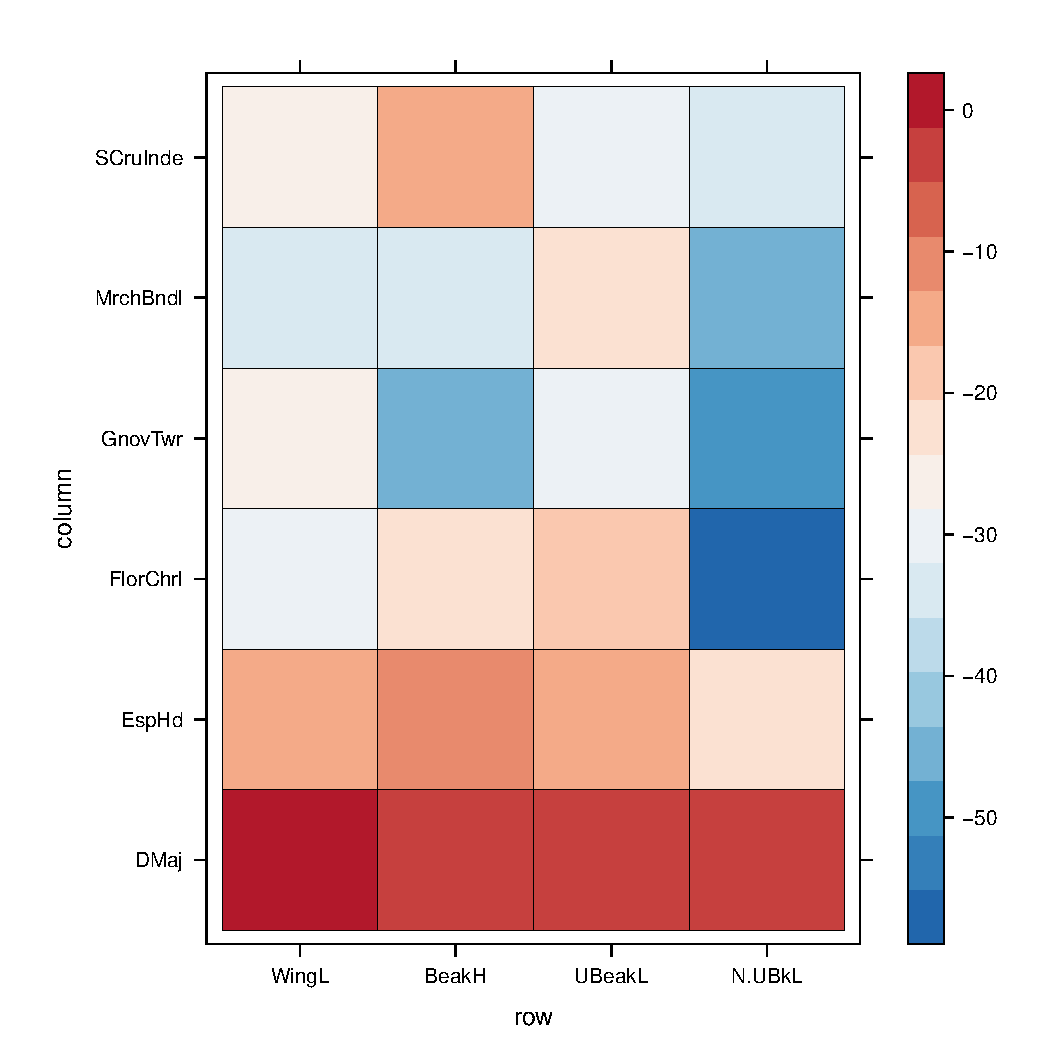
\includegraphics[width=\maxwidth]{figure/unnamed-chunk-551} 
\begin{kframe}\begin{alltt}
\hlkwd{levelplot}\hlstd{(}\hlkwd{cbind}\hlstd{(}\hlkwd{t}\hlstd{(}\hlkwd{ses}\hlstd{(res.finch}\hlopt{$}\hlstd{Tstats}\hlopt{$}\hlstd{T_IP.IC, res.finch}\hlopt{$}\hlstd{Tstats}\hlopt{$}\hlstd{T_IP.IC_nm)}\hlopt{$}\hlstd{ses),}
                \hlkwd{t}\hlstd{(}\hlkwd{ses}\hlstd{(res.finch}\hlopt{$}\hlstd{Tstats}\hlopt{$}\hlstd{T_IC.IR, res.finch}\hlopt{$}\hlstd{Tstats}\hlopt{$}\hlstd{T_IP.IC_nm)}\hlopt{$}\hlstd{ses),}
                \hlkwd{t}\hlstd{(}\hlkwd{ses}\hlstd{(res.finch}\hlopt{$}\hlstd{Tstats}\hlopt{$}\hlstd{T_PC.PR, res.finch}\hlopt{$}\hlstd{Tstats}\hlopt{$}\hlstd{T_IP.IC_nm)}\hlopt{$}\hlstd{ses))}
          \hlstd{,} \hlkwc{colorkey}\hlstd{=my.ckey,} \hlkwc{par.settings}\hlstd{=my.theme,}\hlkwc{border}\hlstd{=}\hlstr{"black"}\hlstd{)}
\end{alltt}
\end{kframe}
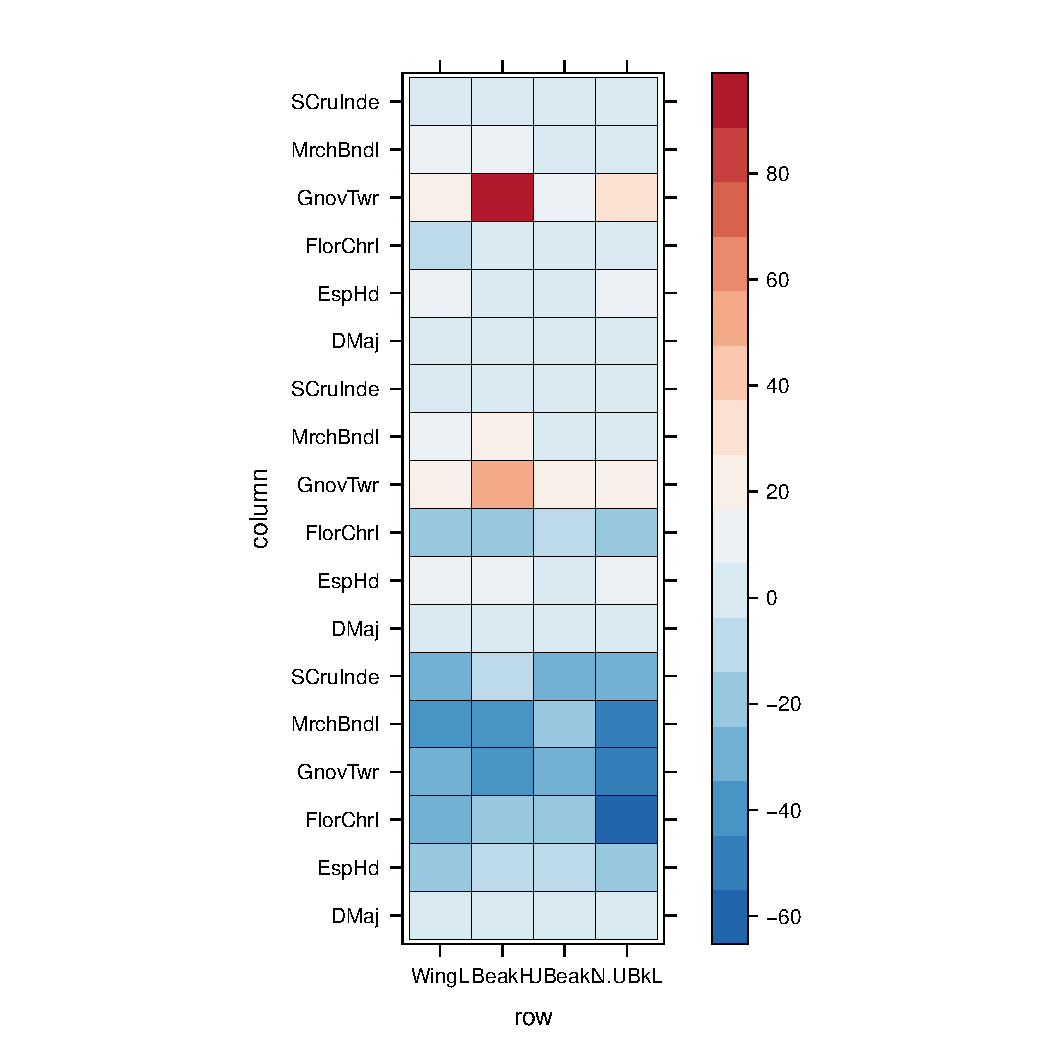
\includegraphics[width=\maxwidth]{figure/unnamed-chunk-552} 

\end{knitrout}

An other example using \tt{ses.listofindex}. The first plot represent "ses" values and the second one the result of a test with H0: observed index value are greater than what we can expect using the null model (alpha=2.5\%).

\begin{knitrout}
\definecolor{shadecolor}{rgb}{0.969, 0.969, 0.969}\color{fgcolor}\begin{kframe}
\begin{alltt}
\hlstd{ses.list}\hlkwb{<-}\hlkwd{ses.listofindex}\hlstd{(i.l1)}

\hlkwd{levelplot}\hlstd{(}\hlkwd{t}\hlstd{(}\hlkwd{rbind}\hlstd{(ses.list[[}\hlnum{1}\hlstd{]]}\hlopt{$}\hlstd{ses, ses.list[[}\hlnum{2}\hlstd{]]}\hlopt{$}\hlstd{ses,}
                  \hlstd{ses.list[[}\hlnum{3}\hlstd{]]}\hlopt{$}\hlstd{ses,  ses.list[[}\hlnum{4}\hlstd{]]}\hlopt{$}\hlstd{ses)),}
          \hlkwc{colorkey}\hlstd{=my.ckey,} \hlkwc{par.settings}\hlstd{=my.theme,}\hlkwc{border}\hlstd{=}\hlstr{"black"}\hlstd{)}
\end{alltt}
\end{kframe}
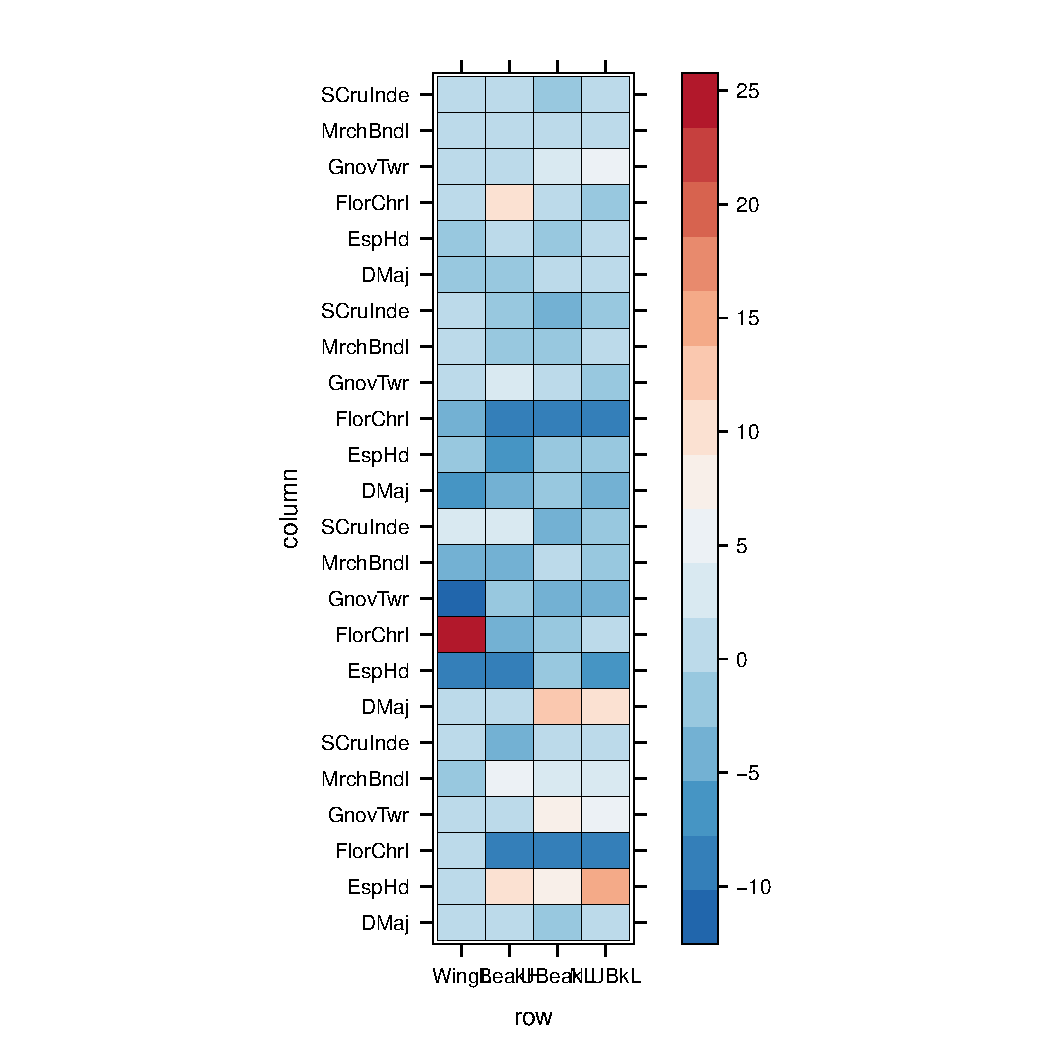
\includegraphics[width=\maxwidth]{figure/unnamed-chunk-561} 
\begin{kframe}\begin{alltt}
\hlkwd{levelplot}\hlstd{(}\hlkwd{t}\hlstd{(}\hlkwd{rbind}\hlstd{(ses.list[[}\hlnum{1}\hlstd{]]}\hlopt{$}\hlstd{ses}\hlopt{>}\hlstd{ses.list[[}\hlnum{1}\hlstd{]]}\hlopt{$}\hlstd{ses.sup,}
                  \hlstd{ses.list[[}\hlnum{2}\hlstd{]]}\hlopt{$}\hlstd{ses}\hlopt{>}\hlstd{ses.list[[}\hlnum{2}\hlstd{]]}\hlopt{$}\hlstd{ses.sup,}
                  \hlstd{ses.list[[}\hlnum{3}\hlstd{]]}\hlopt{$}\hlstd{ses}\hlopt{>}\hlstd{ses.list[[}\hlnum{3}\hlstd{]]}\hlopt{$}\hlstd{ses.sup,}
                  \hlstd{ses.list[[}\hlnum{4}\hlstd{]]}\hlopt{$}\hlstd{ses}\hlopt{>}\hlstd{ses.list[[}\hlnum{4}\hlstd{]]}\hlopt{$}\hlstd{ses.sup)),}
          \hlkwc{colorkey}\hlstd{=my.ckey,} \hlkwc{par.settings}\hlstd{=my.theme,}\hlkwc{border}\hlstd{=}\hlstr{"black"}\hlstd{)}
\end{alltt}
\end{kframe}
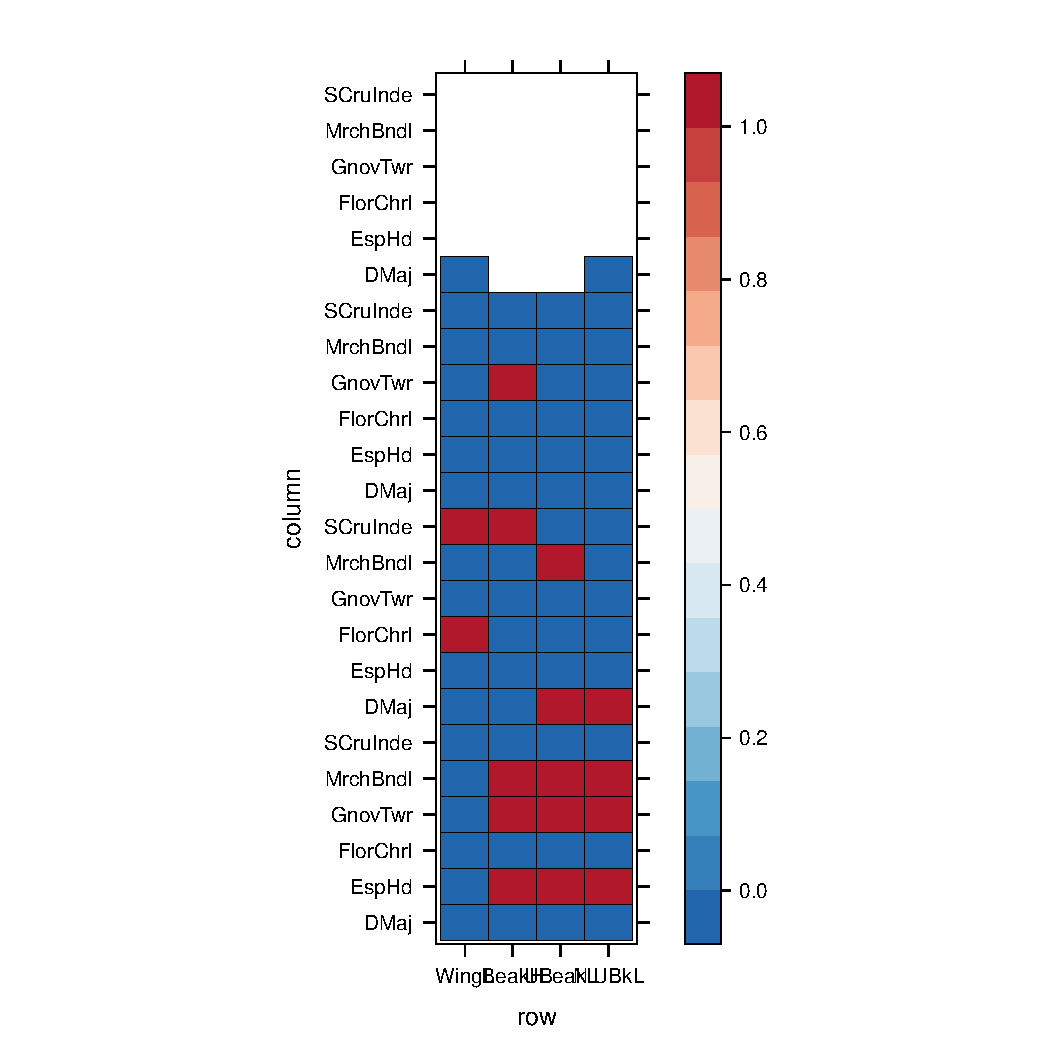
\includegraphics[width=\maxwidth]{figure/unnamed-chunk-562} 

\end{knitrout}

Compare metrics calculate on individual against metrics calculate after populationnal meaning
\begin{knitrout}
\definecolor{shadecolor}{rgb}{0.969, 0.969, 0.969}\color{fgcolor}\begin{kframe}
\begin{alltt}
\hlstd{ses.ind}\hlkwb{<-}\hlkwd{t}\hlstd{(}\hlkwd{rbind}\hlstd{(ses.list[[}\hlnum{1}\hlstd{]]}\hlopt{$}\hlstd{ses,}
           \hlstd{ses.list[[}\hlnum{2}\hlstd{]]}\hlopt{$}\hlstd{ses,}
           \hlstd{ses.list[[}\hlnum{3}\hlstd{]]}\hlopt{$}\hlstd{ses,}
           \hlstd{ses.list[[}\hlnum{4}\hlstd{]]}\hlopt{$}\hlstd{ses))}

\hlstd{ses.sp}\hlkwb{<-}\hlkwd{t}\hlstd{(}\hlkwd{rbind}\hlstd{(ses.list[[}\hlnum{5}\hlstd{]]}\hlopt{$}\hlstd{ses,}
          \hlstd{ses.list[[}\hlnum{6}\hlstd{]]}\hlopt{$}\hlstd{ses,}
          \hlstd{ses.list[[}\hlnum{7}\hlstd{]]}\hlopt{$}\hlstd{ses,}
          \hlstd{ses.list[[}\hlnum{8}\hlstd{]]}\hlopt{$}\hlstd{ses))}

\hlkwd{levelplot}\hlstd{(ses.ind,} \hlkwc{colorkey}\hlstd{=my.ckey,}
          \hlkwc{par.settings}\hlstd{=my.theme,}\hlkwc{border}\hlstd{=}\hlstr{"black"}\hlstd{)}
\end{alltt}
\end{kframe}
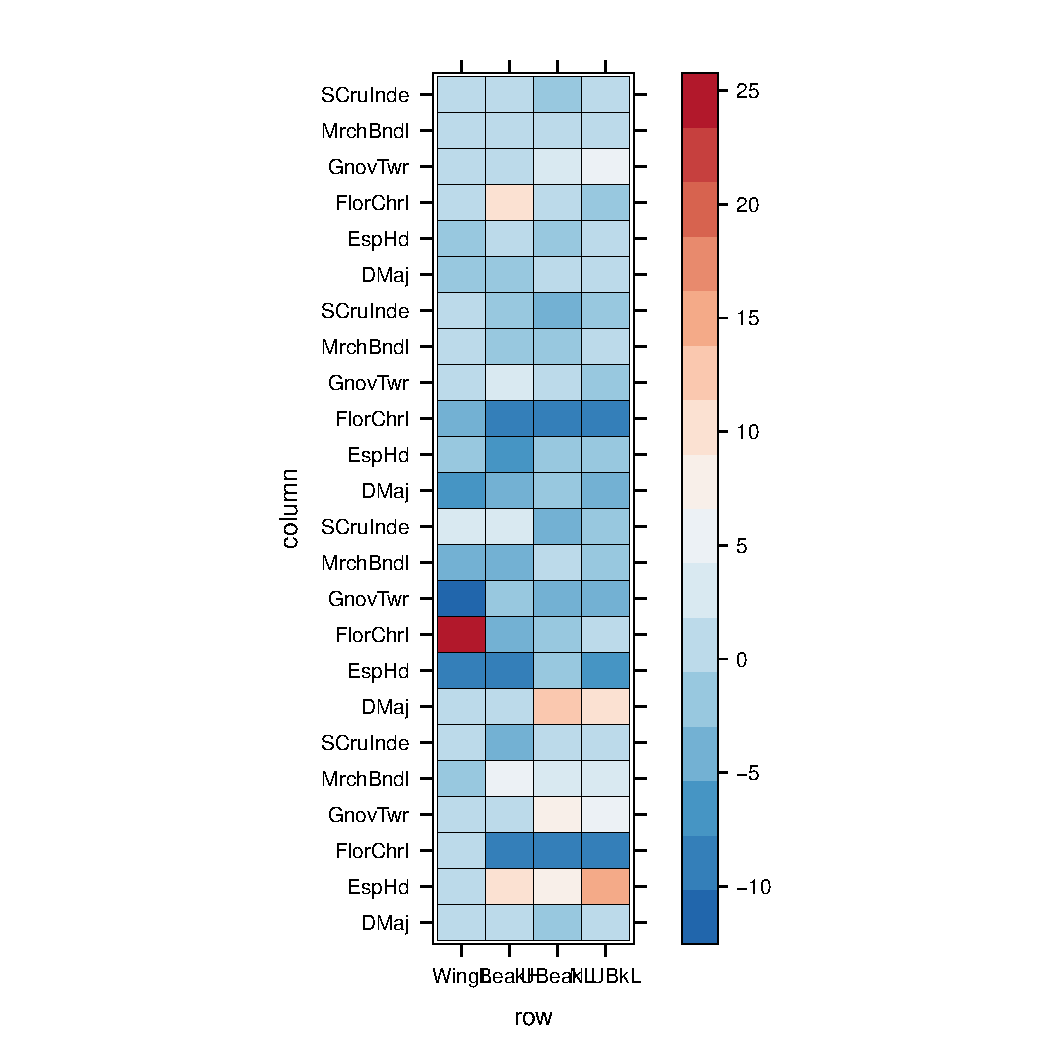
\includegraphics[width=\maxwidth]{figure/unnamed-chunk-571} 
\begin{kframe}\begin{alltt}
\hlkwd{levelplot}\hlstd{(ses.sp,} \hlkwc{colorkey}\hlstd{=my.ckey,}
          \hlkwc{par.settings}\hlstd{=my.theme,}\hlkwc{border}\hlstd{=}\hlstr{"black"}\hlstd{)}
\end{alltt}
\end{kframe}
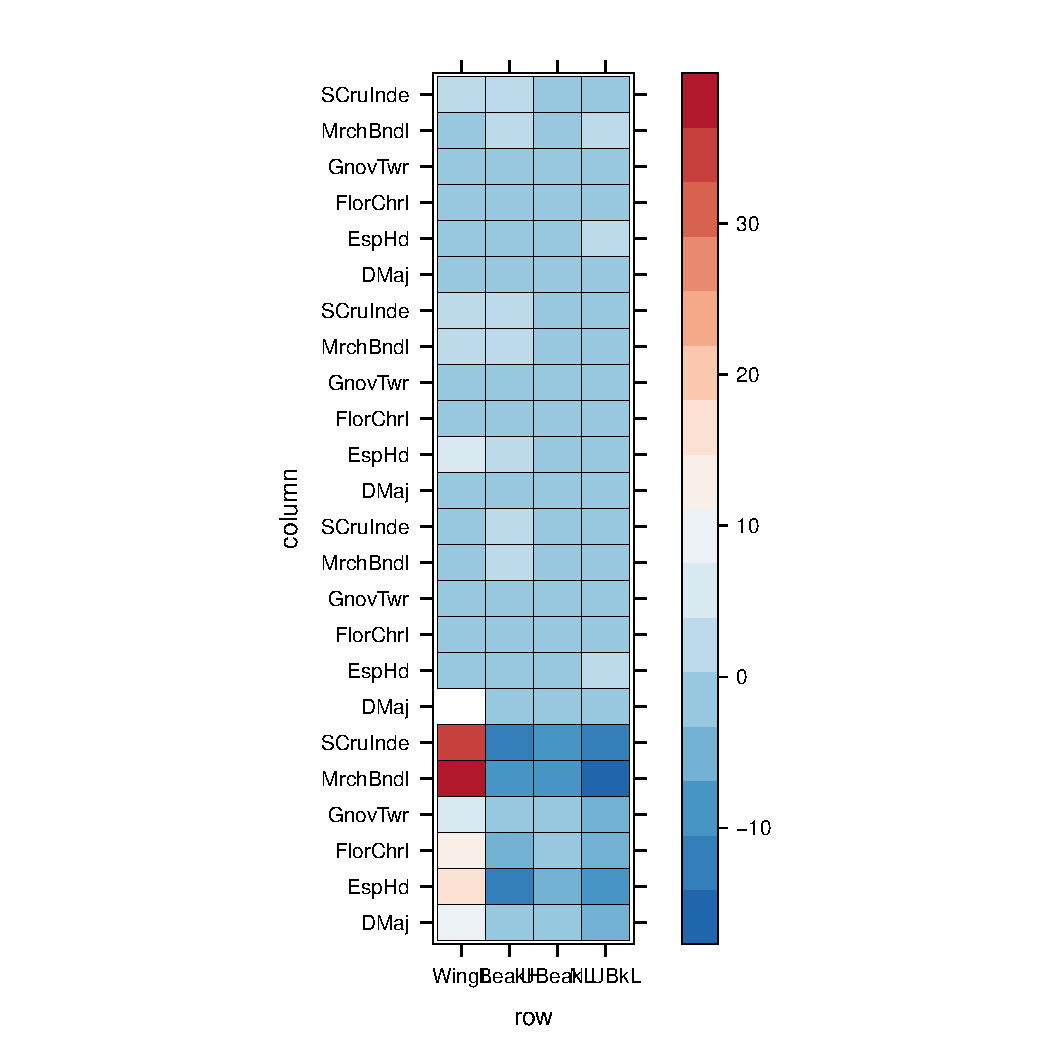
\includegraphics[width=\maxwidth]{figure/unnamed-chunk-572} 

\end{knitrout}

\section{Conclusion}
To finish, we can do a multivariate analysis of the metrics obtain during this tutorial. Analysis dudi 1 put together all traits by meaning the SES values for each metrics in each sites whereas analysis dudi 2 analyse all combination of traits / sites / metrics

\begin{knitrout}
\definecolor{shadecolor}{rgb}{0.969, 0.969, 0.969}\color{fgcolor}\begin{kframe}
\begin{alltt}
\hlkwd{library}\hlstd{(ade4)}

 \hlstd{matfordudi}\hlkwb{<-}\hlkwd{matrix}\hlstd{(}\hlkwc{nrow}\hlstd{=}\hlkwd{length}\hlstd{(}\hlkwd{colMeans}\hlstd{(ses.list[[}\hlnum{1}\hlstd{]]}\hlopt{$}\hlstd{ses)),} \hlkwc{ncol}\hlstd{=}\hlkwd{length}\hlstd{(}\hlkwd{names}\hlstd{(ses.list)))}
 \hlkwa{for}\hlstd{(i} \hlkwa{in} \hlnum{1}\hlopt{:} \hlkwd{length}\hlstd{(}\hlkwd{names}\hlstd{(ses.list)))\{}
   \hlstd{matfordudi[,i]}\hlkwb{<-}\hlkwd{colMeans}\hlstd{(ses.list[[i]]}\hlopt{$}\hlstd{ses)}
 \hlstd{\}}
 \hlkwd{colnames}\hlstd{(matfordudi)}\hlkwb{<-}\hlkwd{names}\hlstd{(ses.list)}
 \hlkwd{rownames}\hlstd{(matfordudi)}\hlkwb{<-}\hlkwd{colnames}\hlstd{(traits.finch)}

 \hlstd{matfordudi2}\hlkwb{<-}\hlkwd{matrix}\hlstd{(}\hlkwc{nrow}\hlstd{=}\hlkwd{length}\hlstd{(}\hlkwd{as.vector}\hlstd{(ses.list[[}\hlnum{1}\hlstd{]]}\hlopt{$}\hlstd{ses)),} \hlkwc{ncol}\hlstd{=}\hlkwd{length}\hlstd{(}\hlkwd{names}\hlstd{(ses.list)))}
 \hlkwa{for}\hlstd{(i} \hlkwa{in} \hlnum{1}\hlopt{:} \hlkwd{length}\hlstd{(}\hlkwd{names}\hlstd{(ses.list)))\{}
   \hlstd{matfordudi2[,i]}\hlkwb{<-}\hlkwd{as.vector}\hlstd{(ses.list[[i]]}\hlopt{$}\hlstd{ses)}
 \hlstd{\}}
 \hlkwd{colnames}\hlstd{(matfordudi2)}\hlkwb{<-}\hlkwd{names}\hlstd{(ses.list)}

\hlcom{#Use mice for the purpose of this example}
\hlstd{matfordudi}\hlkwb{<-}\hlkwd{complete}\hlstd{(}\hlkwd{mice}\hlstd{(matfordudi))}
\end{alltt}
\begin{verbatim}
## 
##  iter imp variable
##   1   1  kurtosis.pop
##   1   2  kurtosis.pop
##   1   3  kurtosis.pop
##   1   4  kurtosis.pop
##   1   5  kurtosis.pop
##   2   1  kurtosis.pop
##   2   2  kurtosis.pop
##   2   3  kurtosis.pop
##   2   4  kurtosis.pop
##   2   5  kurtosis.pop
##   3   1  kurtosis.pop
##   3   2  kurtosis.pop
##   3   3  kurtosis.pop
##   3   4  kurtosis.pop
##   3   5  kurtosis.pop
##   4   1  kurtosis.pop
##   4   2  kurtosis.pop
##   4   3  kurtosis.pop
##   4   4  kurtosis.pop
##   4   5  kurtosis.pop
##   5   1  kurtosis.pop
##   5   2  kurtosis.pop
##   5   3  kurtosis.pop
##   5   4  kurtosis.pop
##   5   5  kurtosis.pop
\end{verbatim}
\begin{alltt}
\hlstd{matfordudi2}\hlkwb{<-}\hlkwd{complete}\hlstd{(}\hlkwd{mice}\hlstd{(matfordudi2))}
\end{alltt}
\begin{verbatim}
## 
##  iter imp variable
##   1   1  kurtosis.pop
##   1   2  kurtosis.pop
##   1   3  kurtosis.pop
##   1   4  kurtosis.pop
##   1   5  kurtosis.pop
##   2   1  kurtosis.pop
##   2   2  kurtosis.pop
##   2   3  kurtosis.pop
##   2   4  kurtosis.pop
##   2   5  kurtosis.pop
##   3   1  kurtosis.pop
##   3   2  kurtosis.pop
##   3   3  kurtosis.pop
##   3   4  kurtosis.pop
##   3   5  kurtosis.pop
##   4   1  kurtosis.pop
##   4   2  kurtosis.pop
##   4   3  kurtosis.pop
##   4   4  kurtosis.pop
##   4   5  kurtosis.pop
##   5   1  kurtosis.pop
##   5   2  kurtosis.pop
##   5   3  kurtosis.pop
##   5   4  kurtosis.pop
##   5   5  kurtosis.pop
\end{verbatim}
\begin{alltt}
\hlstd{res.dudi}\hlkwb{<-}\hlkwd{dudi.pca}\hlstd{(}\hlkwd{t}\hlstd{(matfordudi),} \hlkwc{scan}\hlstd{=F,} \hlkwc{nf}\hlstd{=}\hlnum{2}\hlstd{)}
\hlkwd{s.corcircle}\hlstd{(res.dudi}\hlopt{$}\hlstd{co)}
\hlkwd{s.label}\hlstd{(res.dudi}\hlopt{$}\hlstd{li,} \hlkwc{add.plot}\hlstd{=T,} \hlkwc{clabel} \hlstd{=} \hlnum{0}\hlstd{,} \hlkwc{pch}\hlstd{=}\hlnum{16}\hlstd{)}
\hlkwd{s.label}\hlstd{(res.dudi}\hlopt{$}\hlstd{li}\hlopt{+}\hlnum{0.05}\hlstd{,} \hlkwc{add.plot}\hlstd{=T,} \hlkwc{boxes}\hlstd{=F)}
\end{alltt}
\end{kframe}
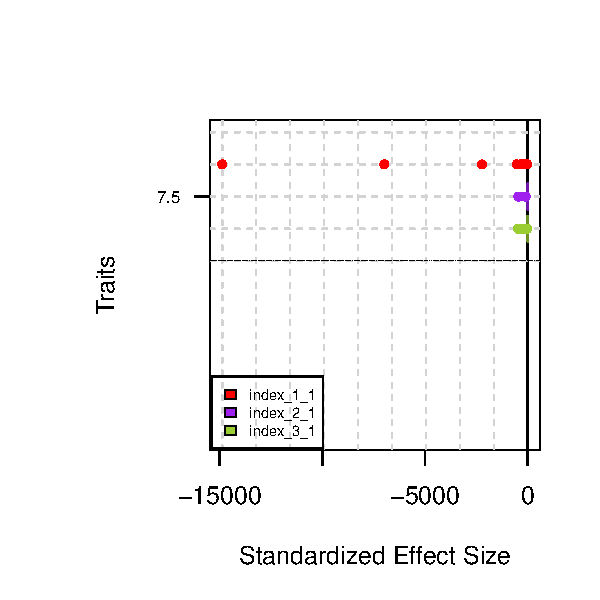
\includegraphics[width=\maxwidth]{figure/unnamed-chunk-581} 
\begin{kframe}\begin{alltt}
\hlstd{res.dudi2}\hlkwb{<-}\hlkwd{dudi.pca}\hlstd{(matfordudi2,} \hlkwc{scan}\hlstd{=F,} \hlkwc{nf}\hlstd{=}\hlnum{2}\hlstd{)}
\hlkwd{scatter}\hlstd{(res.dudi2)}
\end{alltt}
\end{kframe}
\includegraphics[width=\maxwidth]{figure/unnamed-chunk-582} 
\begin{kframe}\begin{alltt}
\hlkwd{s.corcircle}\hlstd{(res.dudi2}\hlopt{$}\hlstd{co)}
\end{alltt}
\end{kframe}
\includegraphics[width=\maxwidth]{figure/unnamed-chunk-583} 
\begin{kframe}\begin{alltt}
\hlkwd{s.class}\hlstd{(res.dudi2}\hlopt{$}\hlstd{li,} \hlkwd{as.factor}\hlstd{(}\hlkwd{c}\hlstd{(}\hlkwd{rep}\hlstd{(}\hlstr{"WingL"}\hlstd{,}\hlnum{6}\hlstd{),} \hlkwd{rep}\hlstd{(}\hlstr{"BeakH"}\hlstd{,}\hlnum{6}\hlstd{),} \hlkwd{rep}\hlstd{(}\hlstr{"UBeakL"}\hlstd{,}\hlnum{6}\hlstd{),} \hlkwd{rep}\hlstd{(}\hlstr{"N.UBkL"}\hlstd{,}\hlnum{6}\hlstd{))),} \hlkwc{col}\hlstd{=}\hlkwd{funky}\hlstd{(}\hlnum{4}\hlstd{))}
\end{alltt}
\end{kframe}
\includegraphics[width=\maxwidth]{figure/unnamed-chunk-584} 
\begin{kframe}\begin{alltt}
\hlkwd{s.class}\hlstd{(res.dudi2}\hlopt{$}\hlstd{li,} \hlkwd{as.factor}\hlstd{(}\hlkwd{rep}\hlstd{(}\hlkwd{c}\hlstd{(}\hlstr{"DMaj"}\hlstd{,}\hlstr{"EspHd"}\hlstd{,}\hlstr{"FlorChrl"}\hlstd{,}\hlstr{"GnovTwr"}\hlstd{,}\hlstr{"MrchBndl"}\hlstd{,}\hlstr{"SCruInde"}\hlstd{),}\hlnum{4} \hlstd{)),} \hlkwc{col}\hlstd{=}\hlkwd{funky}\hlstd{(}\hlnum{6}\hlstd{))}
\end{alltt}
\end{kframe}
\includegraphics[width=\maxwidth]{figure/unnamed-chunk-585} 

\end{knitrout}

\section{Conclusion}
\section{Acknowledgment}

\end{document}







\begin{knitrout}
\definecolor{shadecolor}{rgb}{0.969, 0.969, 0.969}\color{fgcolor}\begin{kframe}
\begin{alltt}
\hlstd{comm}\hlkwb{<-}\hlkwd{t}\hlstd{(}\hlkwd{table}\hlstd{(ind.plot.finch,}\hlnum{1}\hlopt{:}\hlkwd{length}\hlstd{(ind.plot.finch)))}

\hlstd{funct}\hlkwb{<-}\hlkwd{c}\hlstd{(}\hlstr{"spacodi.calc(sp.plot = comm, sp.traits = as.matrix(x) )$Ist"}\hlstd{,}
         \hlstr{"spacodi.calc(sp.plot = comm, sp.traits = as.matrix(x) )$Tst"}  \hlstd{)}
\hlstd{res.finch.sp_mn2}\hlkwb{<-}\hlkwd{ComIndex}\hlstd{(}\hlkwc{traits}\hlstd{=traits.finch.mice,} \hlkwc{index}\hlstd{=funct,} \hlkwc{sp}\hlstd{=sp.finch,}
                            \hlkwc{nullmodels}\hlstd{=}\hlkwd{c}\hlstd{(}\hlnum{2}\hlstd{,}\hlnum{2}\hlstd{,}\hlnum{2}\hlstd{,}\hlnum{2}\hlstd{),} \hlkwc{ind.plot}\hlstd{=ind.plot.finch,}
                            \hlkwc{nperm}\hlstd{=}\hlnum{9}\hlstd{,} \hlkwc{print}\hlstd{=}\hlnum{FALSE}\hlstd{)}
\end{alltt}


{\ttfamily\noindent\bfseries\color{errorcolor}{\#\# Error: impossible de trouver la fonction "{}spacodi.calc"{}}}\begin{alltt}
\hlstd{res.finch.sp_mn3}\hlkwb{<-}\hlkwd{ComIndex}\hlstd{(}\hlkwc{traits}\hlstd{=traits.finch,} \hlkwc{index}\hlstd{=funct,} \hlkwc{sp}\hlstd{=sp.finch,}
                            \hlkwc{nullmodels}\hlstd{=}\hlkwd{c}\hlstd{(}\hlnum{3}\hlstd{,}\hlnum{3}\hlstd{,}\hlnum{3}\hlstd{,}\hlnum{3}\hlstd{),} \hlkwc{ind.plot}\hlstd{=ind.plot.finch,}
                            \hlkwc{nperm}\hlstd{=}\hlnum{9}\hlstd{,} \hlkwc{print}\hlstd{=}\hlnum{FALSE}\hlstd{)}
\end{alltt}
\begin{verbatim}
## [1] "nullmodels need values 1, 2, 2sp or 2sp.prab"
\end{verbatim}


{\ttfamily\noindent\bfseries\color{errorcolor}{\#\# Error: objet 'nm.bis' introuvable}}\end{kframe}
\end{knitrout}

\newpage
We can represent Standardized Effect Size (ses) using the function \tt{plot(as.listofindex(list1, list2, list3))}
\begin{knitrout}
\definecolor{shadecolor}{rgb}{0.969, 0.969, 0.969}\color{fgcolor}\begin{kframe}
\begin{alltt}
\hlstd{list.ind2}\hlkwb{<-}\hlkwd{list}\hlstd{(res.finch.sp_mn2, res.finch.sp_mn3)}
\end{alltt}


{\ttfamily\noindent\bfseries\color{errorcolor}{\#\# Error: objet 'res.finch.sp\_mn3' introuvable}}\begin{alltt}
\hlstd{index.list2}\hlkwb{<-}\hlkwd{as.listofindex}\hlstd{(list.ind2)}
\end{alltt}


{\ttfamily\noindent\bfseries\color{errorcolor}{\#\# Error: objet 'list.ind2' introuvable}}\begin{alltt}
\hlkwd{plot}\hlstd{(index.list2)}
\end{alltt}


{\ttfamily\noindent\bfseries\color{errorcolor}{\#\# Error: erreur d'évaluation de l'argument 'x' lors de la sélection d'une méthode pour la fonction 'plot' : Erreur : objet 'index.list2' introuvable}}\end{kframe}
\end{knitrout}


